%% This is the ctufit-thesis example file. It is used to produce theses
%% for submission to Czech Technical University, Faculty of Information Technology.
%%
%% This is version 1.6.2, built 25. 2. 2026.
%% 
%% Get the newest version from
%% https://gitlab.fit.cvut.cz/theses-templates/FITthesis-LaTeX
%%
%%
%% Copyright 2024, Tomas Novacek
%% Copyright 2021, Eliska Sestakova and Ondrej Guth
%%
%% This work may be distributed and/or modified under the
%% conditions of the LaTeX Project Public License, either version 1.3
%% of this license or (at your option) any later version.
%% The latest version of this license is in
%%  https://www.latex-project.org/lppl.txt
%% and version 1.3 or later is part of all distributions of LaTeX
%% version 2005/12/01 or later.
%%
%% This work has the LPPL maintenance status `maintained'.
%%
%% The current maintainer of this work is Tomas Novacek (novacto3@fit.cvut.cz).
%% Alternatively, submit bug reports to the tracker at
%% https://gitlab.fit.cvut.cz/theses-templates/FITthesis-LaTeX/issues
%%
%%

% arara: xelatex
% arara: biber
% arara: xelatex
% arara: xelatex

%%%%%%%%%%%%%%%%%%%%%%%%%%%%%%%%%%%%%%%%%
% CLASS OPTIONS
% language: czech/english/slovak
% thesis type: bachelor/master/dissertation/doctoral-report
% electronic (oneside) or printed (twoside), twoside is default
% paragraph - if passed, this optional argument sets paragraphs as the deepest level of headers, styles it, numbers it and adds it to Table of Content. Use with care! Normally, it is considered unwise to use it, since it is too deep.
% colour: bw for black&white OR no option for default colour scheme
%%%%%%%%%%%%%%%%%%%%%%%%%%%%%%%%%%%%%%%%%
\documentclass[czech,bachelor,oneside]{ctufit-thesis}

%%%%%%%%%%%%%%%%%%%%%%%%%%%%%%%%%%
% FILL IN THIS INFORMATION
%%%%%%%%%%%%%%%%%%%%%%%%%%%%%%%%%%
\ctufittitle{Software pro evidenci majetku}
\ctufitauthorfull{Ondřej Kopáč}
\ctufitauthorsurnames{Kopáč}
\ctufitauthorgivennames{Ondřej}
\ctufitsupervisor{Ing.\,Jiří Mlejnek}
\ctufitdepartment{Katedra softwarového inženýrství}
\ctufitprogram{Informatika}
\ctufitspecialisation{Softwarové inženýrství}
\ctufityear{2026}
\ctufitdeclarationplace{Praze}
\ctufitdeclarationdate{\today}
\ctufitabstractCZE{Tato bakalářská práce se zabývá návrhem a~implementací systému pro správu majetku. Systém umožňuje evidenci majetkových karet, generování a~tisk etiket s~čárovými kódy, inventarizaci pomocí průmyslové čtečky Zebra a~generování reportů. Skládá se ze tří komponent: serverového REST API (Spring Boot, PostgreSQL), webové aplikace (React, TypeScript) a~mobilní aplikace pro offline inventarizaci (nativní Android, Room). Součástí práce je rešerše existujících řešení, analýza požadavků, volba technologií, návrh architektury, implementace klíčových částí a~testování. Systém je nasazen v~produkčním prostředí pro konkrétní základní školu.}
\ctufitabstractENG{This bachelor's thesis presents the design and implementation of an asset management system. The system enables asset card management, barcode label generation and printing, inventory auditing using a Zebra industrial scanner, and report generation. It consists of three components: a~server-side REST API (Spring Boot, PostgreSQL), a~web application (React, TypeScript), and a~mobile application for offline inventory (native Android, Room). The thesis covers an analysis of existing solutions, requirements specification, technology selection, architecture design, implementation of key features, and testing. The system is deployed in a~production environment for a~specific primary school.}
\ctufitkeywordsCZE{správa majetku, inventarizace, webová aplikace, mobilní aplikace, čárové kódy, tisk etiket, ZPL, Spring Boot, React}
\ctufitkeywordsENG{asset management, inventory, web application, mobile application, barcodes, label printing, ZPL, Spring Boot, React}
%%%%%%%%%%%%%%%%%%%%%%%%%%%%%%%%%%
% END FILL IN
%%%%%%%%%%%%%%%%%%%%%%%%%%%%%%%%%%

%%%%%%%%%%%%%%%%%%%%%%%%%%%%%%%%%%
% CUSTOMIZATION of this template
% Skip this part or alter it if you know what you are doing.
%%%%%%%%%%%%%%%%%%%%%%%%%%%%%%%%%%

\RequirePackage{iftex}[2020/03/06]
\iftutex % XeLaTeX and LuaLaTeX
    \RequirePackage{ellipsis}[2020/05/22] %ellipsis workaround for XeLaTeX
\else
    \errmessage{Only compilation with XeLaTeX or LuaLaTeX is allowed}
    \stop
\fi

% hyperlinks
\hypersetup{
    pdfpagelayout=TwoPageRight,
    colorlinks=false,
    allcolors=decoration,
    pdfborder={0 0 0.1}
}

% uncomment the following to hide all hyperlinks
%\hypersetup{hidelinks}

% uncomment the following to change the colour of all hyperlinks to CTU blue
%\hypersetup{allbordercolors=decoration}

\RequirePackage{pdfpages}[2020/01/28]

%%%%%%%%%%%%%%%%%%%%%%%%%%%%%%%%%%
% CUSTOMIZATION of this template END
%%%%%%%%%%%%%%%%%%%%%%%%%%%%%%%%%%


%%%%%%%%%%%%%%%%%%%%%%
% PACKAGES SETTINGS
% You may choose to modify this part.
%%%%%%%%%%%%%%%%%%%%%%
\usepackage{dirtree}
\usepackage{lipsum,tikz}
\usepackage[style=iso-numeric]{biblatex}
\addbibresource{text/bib-database.bib}
\usepackage{xurl}
\usepackage{listings} % typesetting of sources
\AddToHook{begindocument/end}{%
  \lstset{
    keywordstyle=\color[rgb]{0,0,0.6}\bfseries,
    commentstyle=\color[rgb]{0,0.5,0}\itshape,
    stringstyle=\color[rgb]{0.64,0.08,0.08},
    showstringspaces=false,
    backgroundcolor=\color{white},
  }%
}
\lstdefinelanguage{TypeScript}{
  keywords={const, let, var, function, return, if, else, for, while, do, switch, case, break, continue, new, throw, try, catch, finally, typeof, instanceof, in, of, class, extends, implements, interface, type, export, import, from, default, async, await, yield, readonly, enum, as, null, undefined, true, false, void},
  sensitive=true,
  morecomment=[l]{//},
  morecomment=[s]{/*}{*/},
  morestring=[b]",
  morestring=[b]',
  morestring=[b]`,
}
\usepackage{minted}
\usemintedstyle{friendly}
\AtBeginEnvironment{minted}{\renewcommand{\fcolorbox}[4][]{#4}}
\counterwithin{listing}{chapter}
\usepackage{csquotes}
\usepackage{needspace}
\usepackage{float}

\hyphenation{
	backend backendu backende backendem
	frontend frontendu frontende frontendem
	framework frameworky frameworků frameworkem
	TypeScript TypeScriptu TypeScriptem TypeScriptový TypeScriptových TypeScriptové
	JavaScript JavaScriptu JavaScriptem JavaScriptový JavaScriptových JavaScriptové
	EasyExcel
	Vuetify
	MapStruct
	PostgreSQL
	boilerplate
	lifecycle
	toolchain
	opinionated neopinionated
	cleartext
	refetch refetching
	interceptor
	business
	listenerů listenery listenerům
	features
	Specification
	fulltextové fulltextového fulltextovým
	React Reactu Reactem
}

% Povolit LaTeXu mírně roztáhnout mezery místo přetečení řádku
\emergencystretch=2em

%%%%%%%%%%%%%%%%%%%%%%
% PACKAGES SETTINGS END
%%%%%%%%%%%%%%%%%%%%%%

\begin{document}
\frontmatter\frontmatterinit % do not remove these two commands

\thispagestyle{empty}\maketitle\thispagestyle{empty}\cleardoublepage % do not remove these four commands

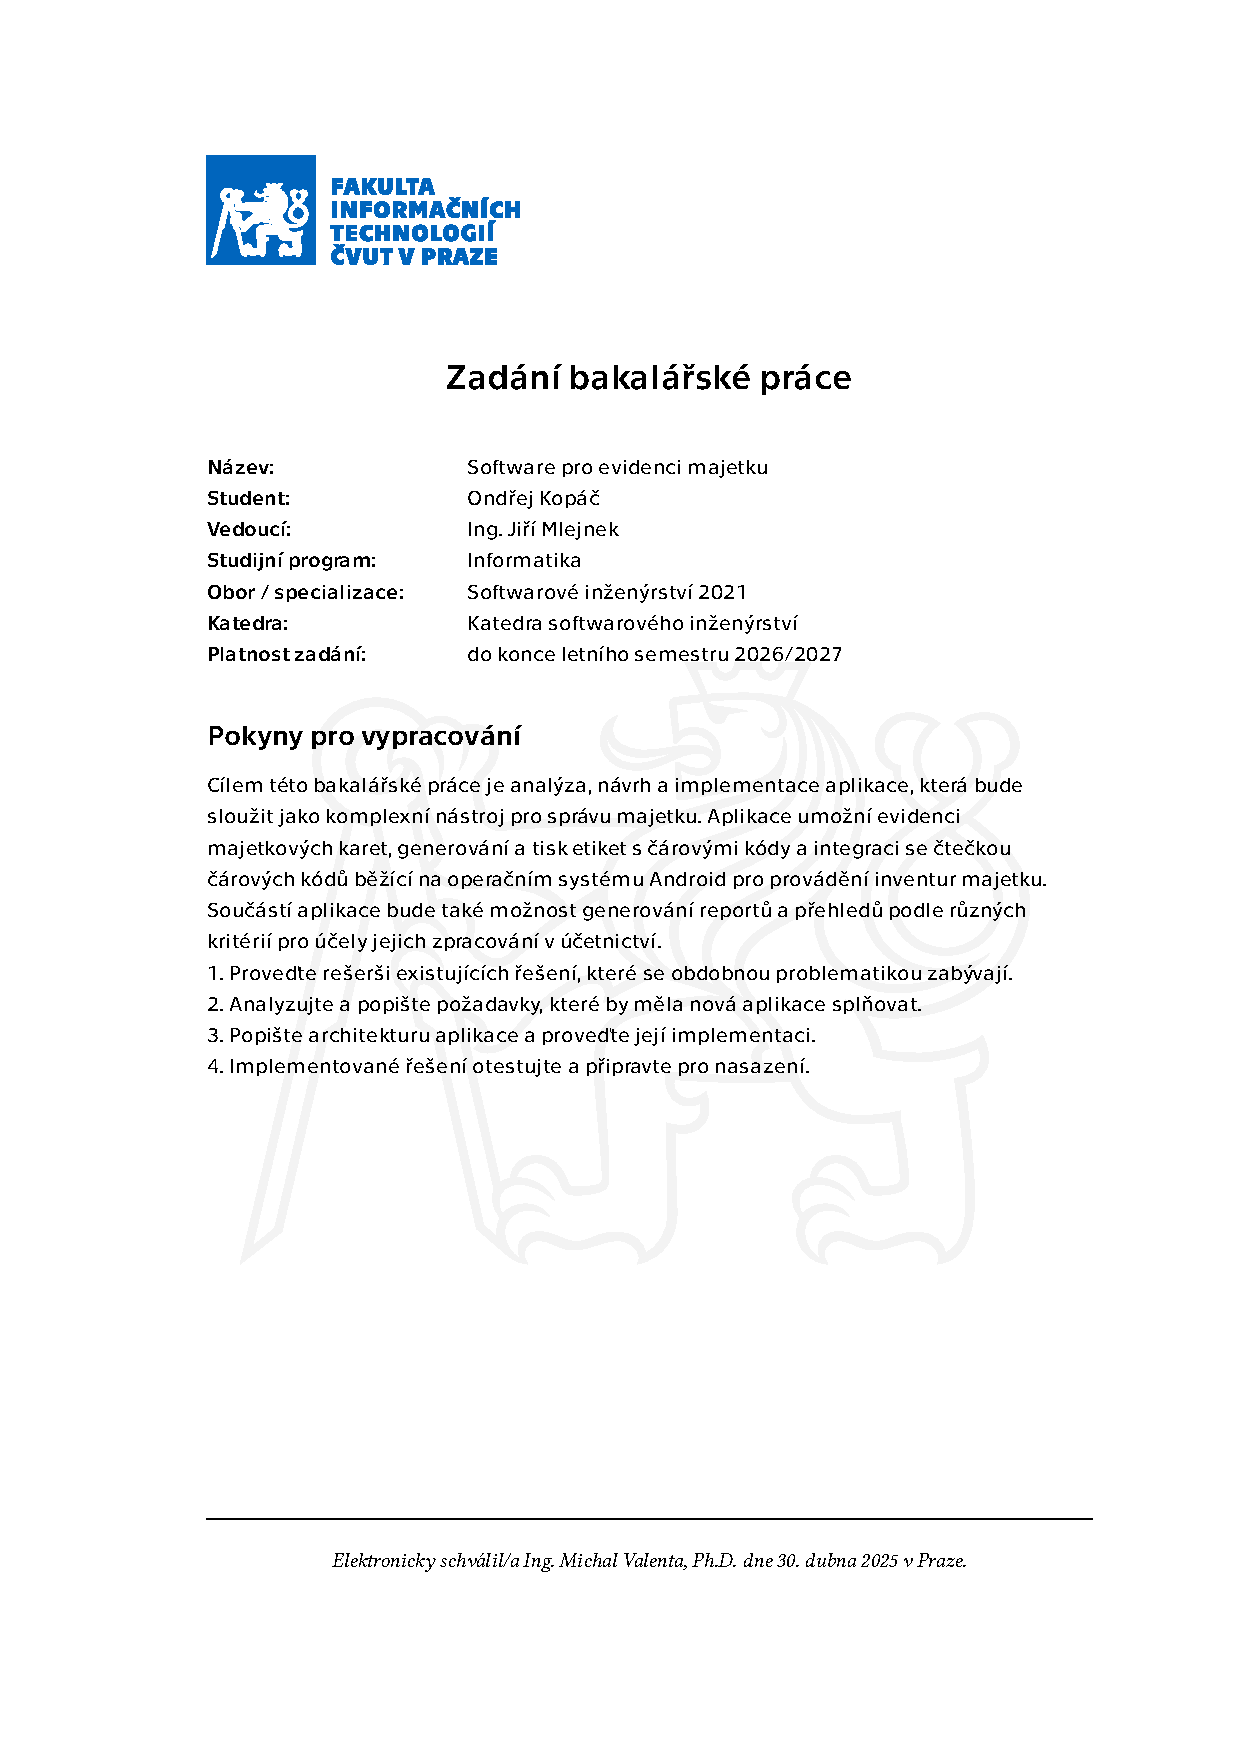
\includepdf[pages={1-}]{assignment-include.pdf}

\imprintpage % do not remove this command
\stopTOCentries

%%%%%%%%%%%%%%%%%%%
% ACKNOWLEDGMENT
% FILL IN / MODIFY
% This is a place to thank people for helping you. It is common to thank your supervisor.
%%%%%%%%%%%%%%%%%%%
\begin{acknowledgmentpage}
	Chtěl bych poděkovat především sit amet, consectetuer adipiscing elit. Curabitur sagittis hendrerit ante. Class aptent taciti sociosqu ad litora torquent per conubia nostra, per inceptos hymenaeos. Cras pede libero, dapibus nec, pretium sit amet, tempor quis. Sed vel lectus. Donec odio tempus molestie, porttitor ut, iaculis quis, sem. Suspendisse sagittis ultrices augue.
\end{acknowledgmentpage}
%%%%%%%%%%%%%%%%%%%
% ACKNOWLEDGMENT END
%%%%%%%%%%%%%%%%%%%


%%%%%%%%%%%%%%%%%%%
% DECLARATION
% FILL IN / MODIFY
%%%%%%%%%%%%%%%%%%%
% INSTRUCTIONS
% ENG: choose one of approved texts of the declaration. DO NOT CREATE YOUR OWN. Find the approved texts at https://courses.fit.cvut.cz/SFE/download/index.html#_documents (document Declaration for FT in English)
% CZE/SLO: Vyberte jedno z fakultou schvalenych prohlaseni. NEVKLADEJTE VLASTNI TEXT. Schvalena prohlaseni najdete zde: https://courses.fit.cvut.cz/SZZ/dokumenty/index.html#_dokumenty (prohlášení do ZP)
\begin{declarationpage}
	Prohlašuji, že jsem předloženou práci vypracoval samostatně a~že jsem uvedl veškeré použité informační zdroje v~souladu s~Metodickým pokynem o~dodržování etických principů při přípravě vysokoškolských závěrečných prací.

	Beru na vědomí, že se na moji práci vztahují práva a~povinnosti vyplývající ze zákona č.~121/2000~Sb., autorského zákona, ve znění pozdějších předpisů, zejména skutečnost, že České vysoké učení technické v~Praze má právo na uzavření licenční smlouvy o~užití této práce jako školního díla podle §~60 odst.~1 citovaného zákona.
\end{declarationpage}
%%%%%%%%%%%%%%%%%%%
% DECLARATION END
%%%%%%%%%%%%%%%%%%%

% Use one of the two following commands. The first prints abstracts+keywords on two pages, the second puts them on one page (if possible). \printonepageabstract can also accept optional argument that specifies a vertical space before both abstracts (the default is 18 mm).
\printtwopageabstract
%\printonepageabstract 

%%%%%%%%%%%%%%%%%%%
% SUMMARY
% FILL IN / MODIFY
% OR REMOVE ENTIRELY (upon agreement with your supervisor)
% (appropriate to remove in most theses)
%%%%%%%%%%%%%%%%%%%
% \begin{summarypage}
% \section*{Summary section}
% 
% \lipsum[1][1-8]
% 
% \section*{Summary section}
% 
% \lipsum[2][1-6]
% 
% \section*{Summary section}
% 
% \lipsum[3]
% 
% \section*{Summary section}
% 
% \lipsum[2]
% 
% \section*{Summary section}
% 
% \lipsum[1][1-8] Lorem lorem lorem.
% \end{summarypage}
%%%%%%%%%%%%%%%%%%%
% SUMMARY END
%%%%%%%%%%%%%%%%%%%

\tableofcontents % do not remove this command
%%%%%%%%%%%%%%%%%%%%%%
% list of other contents: figures, tables, code listings, algorithms, etc.
% add/remove commands accordingly
%%%%%%%%%%%%%%%%%%%%%%
\listoffigures % list of figures
\begingroup
\let\clearpage\relax
\listoftables % list of tables. Remove if you do not have any.
\thectufitlistingscommand{} % list of code listings. Remove if you do not have any.
\thectufitlistofalgorithmscommand{} % list of algorithm pseudocodes defined using the algorithm package.
\endgroup
%%%%%%%%%%%%%%%%%%%%%%
% list of other contents END
%%%%%%%%%%%%%%%%%%%%%%

%%%%%%%%%%%%%%%%%%%
% ABBREVIATIONS
% FILL IN / MODIFY
% OR REMOVE ENTIRELY
% List the abbreviations in lexicography order.
%%%%%%%%%%%%%%%%%%%
\chapter{\thectufitabbreviationlabel}

\begin{tabular}{rl}
	APK    & Android Package Kit                             \\
	API    & Application Programming Interface               \\
	CI/CD  & Continuous Integration / Continuous Deployment   \\
	AES    & Advanced Encryption Standard                     \\
	CRUD   & Create, Read, Update, Delete                    \\
	CSRF   & Cross-Site Request Forgery                      \\
	CSS    & Cascading Style Sheets                          \\
	DAO    & Data Access Object                              \\
	DB     & Database                                        \\
	DTO    & Data Transfer Object                            \\
	FK     & Foreign Key                                     \\
	GCM    & Galois/Counter Mode                             \\
	HTML   & HyperText Markup Language                       \\
	HTTP   & HyperText Transfer Protocol                     \\
	HTTPS  & HyperText Transfer Protocol Secure              \\
	HW     & Hardware                                        \\
	JSON   & JavaScript Object Notation                      \\
	JPA    & Jakarta Persistence API                         \\
	JVM    & Java Virtual Machine                            \\
	JWT    & JSON Web Token                                  \\
	KMP    & Kotlin Multiplatform                            \\
	MUI    & Material UI                                     \\
	ORM    & Object-Relational Mapping                       \\
	PDF    & Portable Document Format                        \\
	PK     & Primary Key                                     \\
	REST   & Representational State Transfer                 \\
	RN     & React Native                                    \\
	SPA    & Single Page Application                         \\
	SQL    & Structured Query Language                       \\
	SSH    & Secure Shell                                    \\
	SSL    & Secure Sockets Layer                            \\
	UI     & User Interface                                  \\
	VPS    & Virtual Private Server                          \\
	XLSX   & Excel Open XML Spreadsheet                      \\
	ZPL    & Zebra Programming Language
\end{tabular}
%%%%%%%%%%%%%%%%%%%
% ABBREVIATIONS END
%%%%%%%%%%%%%%%%%%%
\resumeTOCentries
\mainmatter\mainmatterinit % do not remove these two commands
%%%%%%%%%%%%%%%%%%%
% THE THESIS
% MODIFY ANYTHING BELOW THIS LINE
%%%%%%%%%%%%%%%%%%%

\chapter{Úvod}
\setcounter{page}{1}

Správa majetku je nedílnou součástí provozu každé organizace. Zahrnuje evidenci hmotných položek, sledování jejich umístění, stavu a~životního cyklu od pořízení přes inventarizaci až po vyřazení. V~mnoha organizacích, zejména ve školách a~menších institucích, je tato evidence vedena v~tabulkových procesorech bez systematické podpory inventarizace.

Tato práce vznikla na základě konkrétní potřeby Základní školy Ústavní v~Praze~8, která dosud evidovala majetek v~tabulkách aplikace Microsoft Excel. Při tisících položek rozmístěných v~desítkách místností je ruční inventura časově náročná a~náchylná k~chybám. Škola proto hledala řešení, které by umožnilo automatizovanou inventarizaci pomocí čtečky čárových kódů, generování etiket pro označení majetku a~přehlednou správu evidence prostřednictvím webové aplikace.

Cílem práce je navrhnout a~implementovat webový systém pro správu majetku s~mobilní aplikací pro offline inventuru v~terénu. Systém má umožnit evidenci majetkových karet, generování a~tisk etiket s~čárovými kódy, sběr inventurních dat pomocí průmyslové čtečky Zebra a~vyhodnocení inventury včetně generování reportů.

\medskip

Práce je strukturována následovně. Kapitola~\ref{chap:research} analyzuje existující přístupy ke~správě majetku a~zdůvodňuje vývoj vlastního řešení. Kapitola~\ref{chap:requirements} definuje funkční a~obecné požadavky a~popisuje případy užití. Kapitola~\ref{chap:technologies} srovnává technologie a~zdůvodňuje jejich volbu. Kapitola~\ref{chap:architecture} popisuje návrh architektury systému včetně datového modelu. Kapitola~\ref{chap:implementation} se zaměřuje na klíčové implementační detaily. Kapitola~\ref{chap:testing} pokrývá testování a~nasazení do produkčního prostředí. Kapitola~\ref{chap:conclusion} shrnuje dosažené výsledky a~navrhuje možnosti dalšího rozvoje.



\chapter{Rešerše existujících řešení}\label{chap:research}

\begin{chapterabstract}
	Tato kapitola analyzuje existující přístupy ke~správě majetku a~inventarizaci. Srovnání slouží jako základ pro definici požadavků na vlastní řešení.
\end{chapterabstract}

Před zahájením vývoje vlastního systému byly prozkoumány dostupné způsoby evidence majetku -- od tabulkových procesorů přes komerční specializované systémy až po open-source řešení.

\section{Tabulkové procesory}

Cílová organizace (základní škola) dosud evidovala majetek v~tabulkovém procesoru Microsoft Excel. Tento přístup nevyžaduje žádné dodatečné náklady a~je snadno dostupný. Umožňuje základní operace -- seznam majetku, filtrování a~řazení.

Zásadní nevýhodou je absence podpory pro inventarizaci s~čtečkou čárových kódů. Inventura probíhala ručním porovnáváním vytištěných seznamů se skutečným stavem, což je při tisících položek časově náročné a~náchylné k~chybám. Tabulkový procesor dále neposkytuje historii změn, správu uživatelských rolí ani možnost generování etiket s~identifikačními kódy.

\section{Komerční řešení}

Na trhu existuje řada komerčních systémů pro evidenci a~inventarizaci majetku. Následující sekce popisují dvě řešení, která byla zvažována pro cílovou organizaci.

\subsection{EVIDEI}

EVIDEI~\cite{evidei} je specializovaný systém pro evidenci a~inventarizaci majetku vyvíjený českou společností KODYS~\cite{kodys}, která je zároveň certifikovaným partnerem výrobce Zebra Technologies. Systém je provozován jako cloudová služba na platformě Microsoft Azure s~mobilní aplikací pro iOS a~Android.

EVIDEI nabízí kompletní životní cyklus majetku -- od založení karty přes přesuny a~inventury až po vyřazení. Podporuje identifikaci pomocí čárových kódů (1D i~2D), QR kódů a~RFID technologie. Mobilní aplikace umožňuje skenování přímo prostřednictvím průmyslových terminálů Zebra nebo běžných mobilních zařízení. Součástí je také foto dokumentace, víceúrovňové členění umístění a~integrace s~ERP systémy prostřednictvím API.

Cena systému není veřejně dostupná a~závisí na počtu spravovaných položek a~délce předplatného. Cílová organizace obdržela cenovou nabídku, která však přesahovala její rozpočtové možnosti.

\subsection{Správce Majetku}

Správce Majetku~\cite{spravce-majetku} je české webové řešení pro evidenci majetku s~podporou QR kódů. Aplikace je přístupná prostřednictvím webového prohlížeče a~nabízí kategorizaci majetku, sledování umístění, plánování údržby a~automatické připomínky revizí.

Systém nabízí zvýhodněný tarif pro školy a~veřejné instituce. Cena se odvíjí od počtu uživatelů a~spravovaných položek; pro organizace s~větším rozsahem majetku je k~dispozici individuální nabídka. Identifikace majetku probíhá prostřednictvím QR kódů snímaných kamerou běžného mobilního telefonu.

Nevýhodou je absence podpory průmyslových čtecích terminálů Zebra a~offline režimu -- aplikace vyžaduje stálé připojení k~internetu. Pro organizaci disponující dedikovaným hardwarem Zebra tak není plně využitelná.

\section{Open-source řešení}

Alternativou ke komerčním produktům jsou open-source systémy, které lze provozovat na vlastním serveru bez licenčních poplatků.

\subsection{Snipe-IT}

Snipe-IT~\cite{snipeit} je nejrozšířenější open-source systém pro správu majetku, dostupný pod licencí MIT~\cite{snipeit-github}. Je implementován v~jazyce PHP s~využitím frameworku Laravel. Systém lze provozovat na vlastním serveru zdarma, případně využít placenou cloudovou variantu (od 39,99~USD měsíčně).

Snipe-IT podporuje generování QR a~čárových kódů, nabízí REST API, kompletní audit log a~lokalizaci do více než 55 jazyků. Mobilní přístup je realizován prostřednictvím responzivního webového rozhraní; nativní mobilní aplikace pro offline inventuru není součástí projektu.

Hlavní nevýhodou pro účely tohoto projektu je zaměření primárně na IT majetek (počítače, licence, příslušenství). Systém neposkytuje nativní podporu pro průmyslové čtečky Zebra ani offline režim při inventuře v~terénu. Provoz na vlastním serveru navíc vyžaduje průběžnou údržbu a~aktualizace.

\section{Srovnání a~zdůvodnění vlastního řešení}

Tabulka~\ref{tab:comparison} shrnuje srovnání analyzovaných řešení s~vlastním systémem podle klíčových kritérií vycházejících z~potřeb cílové organizace.

\begin{table}[H]\centering\footnotesize
\renewcommand{\arraystretch}{1.3}
\begin{tabular}{l|c|c|c|c|c}
	\textbf{Kritérium} & \textbf{Excel} & \textbf{EVIDEI} & \textbf{Správce M.} & \textbf{Snipe-IT} & \textbf{Vlastní} \tabularnewline \hline
	Cena & zdarma & na dotaz & na dotaz & zdarma & zdarma \tabularnewline
	Inventura s~čtečkou & ne & ano & ne & ne & ano \tabularnewline
	Offline režim & -- & ano & ne & ne & ano \tabularnewline
	Tisk ZPL etiket & ne & ano & ne & ne & ano \tabularnewline
	Český jazyk & ano & ano & ano & částečně & ano \tabularnewline
	Webové rozhraní & ne & ano & ano & ano & ano \tabularnewline
	Přizpůsobitelnost & -- & ne & ne & částečně & ano \tabularnewline
\end{tabular}
\caption{Srovnání existujících řešení pro správu majetku}\label{tab:comparison}
\end{table}

Žádné z~analyzovaných řešení nepokrývá všechny potřeby cílové organizace za přijatelnou cenu. Tabulkový procesor postrádá podporu inventarizace. Komerční systém EVIDEI nabízí požadovanou funkcionalitu včetně integrace se Zebra zařízeními, ale jeho cena přesahuje rozpočet základní školy. Správce Majetku je cenově dostupný, ale nepodporuje průmyslové čtečky ani offline inventuru. Snipe-IT je zaměřen na IT majetek a~postrádá offline mobilní aplikaci.

Volba dedikované průmyslové čtečky Zebra TC22 místo běžného mobilního telefonu s~kamerou je motivována povahou inventarizace -- při skenování tisíců položek je hardwarový skener výrazně rychlejší a~spolehlivější než kamera telefonu, zejména u~poškozených nebo špatně přístupných štítků. Enterprise zařízení je navíc odolnější vůči náročnějším podmínkám ve~školním prostředí (sklady, dílny). Offline režim je nezbytný, protože Wi-Fi pokrytí v~budově školy není úplné a~mobilní data nemusí být ve~všech prostorách dostupná.

Na základě tohoto srovnání bylo rozhodnuto o~vývoji vlastního řešení, které přesně odpovídá požadavkům organizace -- včetně integrace s~hardwarem Zebra (čtečka TC22, tiskárna ZD621d), offline inventury a~generování ZPL etiket.



\chapter{Analýza požadavků}\label{chap:requirements}

\begin{chapterabstract}
	Kapitola definuje funkční a~obecné požadavky na vyvíjený systém. Požadavky vycházejí ze~zadání práce, z~potřeb cílové organizace a~z~analýzy existujících řešení.
\end{chapterabstract}

Systém byl vyvíjen jako zakázka pro konkrétní základní školu, která dosud evidovala majetek v~tabulkových procesorech bez systematické inventarizace. Požadavky byly stanoveny na základě konzultací s~budoucími uživateli systému (účetní a~hospodářka školy) a~průběžně upřesňovány během vývoje.

\section{Funkční požadavky}

Požadavky jsou rozděleny do logických skupin a~každý má jedinečný identifikátor, na nějž se odkazují další kapitoly (zejména kapitola~\ref{chap:implementation}).

\subsection{Evidence majetkových karet}

Majetková karta je základní datová jednotka systému. Každá karta reprezentuje jednu položku majetku a~nese informace potřebné pro účetní evidenci.

\begin{table}[H]\centering
\renewcommand{\arraystretch}{1.4}
\caption{Funkční požadavky -- evidence majetkových karet}\label{tab:freq-cards}
\begin{tabular}{l|p{10cm}}
	\textbf{ID} & \textbf{Popis požadavku} \tabularnewline \hline
	F-01 & Systém umožní vytvořit novou majetkovou kartu s~atributy: název, cena, počet kusů, sériové číslo, umístění, třída, skupina majetku, způsob pořízení, faktura, datum pořízení, zodpovědná osoba a~poznámka. \tabularnewline
	F-02 & Systém umožní zobrazit, upravit a~smazat existující majetkovou kartu. \tabularnewline
	F-03 & Systém umožní duplikovat existující kartu pro usnadnění hromadného zadávání podobného majetku. \tabularnewline
	F-04 & Systém umožní filtrovat karty podle libovolné kombinace atributů (identifikátor, název, rozsah ceny, umístění, třída, skupina, datum pořízení, datum vyřazení a~další). \tabularnewline
	F-05 & Systém umožní fulltextové vyhledávání v~kartách majetku. \tabularnewline
	F-06 & Systém umožní nahrávat, stahovat a~mazat souborové přílohy ke~kartám majetku. \tabularnewline
	F-07 & Systém umožní vyřadit majetkovou kartu zadáním data a~způsobu vyřazení. \tabularnewline
\end{tabular}
\end{table}

\subsection{Správa číselníků}

Číselníky definují přípustné hodnoty pro atributy majetkových karet. Systém pracuje s~pěti číselníky: umístění (místnosti), skupiny majetku, třídy majetku, způsoby pořízení a~způsoby vyřazení.

\begin{table}[H]\centering
\renewcommand{\arraystretch}{1.4}
\caption{Funkční požadavky -- správa číselníků}\label{tab:freq-dictionaries}
\begin{tabular}{l|p{10cm}}
	\textbf{ID} & \textbf{Popis požadavku} \tabularnewline \hline
	F-08 & Systém umožní vytvořit, přejmenovat a~smazat položku v~každém z~pěti číselníků (umístění, skupiny, třídy, způsoby pořízení, způsoby vyřazení). \tabularnewline
\end{tabular}
\end{table}

\subsection{Generování a~tisk etiket}

Etikety s~Data Matrix kódy slouží k~fyzické identifikaci majetku a~místností. Systém generuje etikety ve~formátu ZPL (Zebra Programming Language), který je nativním jazykem tiskáren Zebra.

\begin{table}[H]\centering
\renewcommand{\arraystretch}{1.4}
\caption{Funkční požadavky -- generování a~tisk etiket}\label{tab:freq-labels}
\begin{tabular}{l|p{10cm}}
	\textbf{ID} & \textbf{Popis požadavku} \tabularnewline \hline
	F-09 & Systém umožní generovat ZPL etikety s~Data Matrix kódem pro majetkové karty. Etiketa obsahuje identifikátor karty, název majetku a~název organizace. \tabularnewline
	F-10 & Systém umožní hromadný tisk etiket pro vybrané karty majetku. \tabularnewline
	F-11 & Systém umožní generovat ZPL etikety pro místnosti (číselník umístění). \tabularnewline
\end{tabular}
\end{table}

\subsection{Reporty a~exporty}

Systém umožňuje generovat přehledy a~sestavy ve~formátu PDF a~Excel pro potřeby účetní evidence a~kontroly majetku.

\begin{table}[H]\centering
\renewcommand{\arraystretch}{1.4}
\caption{Funkční požadavky -- reporty a~exporty}\label{tab:freq-reports}
\begin{tabular}{l|p{10cm}}
	\textbf{ID} & \textbf{Popis požadavku} \tabularnewline \hline
	F-12 & Systém umožní generovat PDF sestavu pro vybranou skupinu majetku (nebo všechny skupiny) k~zadanému datu. \tabularnewline
	F-13 & Systém umožní generovat PDF sestavu majetku pro vybranou místnost. \tabularnewline
	F-14 & Systém umožní generovat PDF sestavu pro konkrétní majetkovou kartu. \tabularnewline
	F-15 & Systém umožní exportovat filtrované karty majetku do~formátu Excel (XLSX). \tabularnewline
\end{tabular}
\end{table}

\subsection{Inventura}

Inventura je klíčový proces, při kterém se ověřuje skutečný stav majetku oproti evidenčnímu stavu. Proces probíhá ve~třech fázích: sběr dat v~terénu (mobilní aplikace), přenos dat na server a~vyhodnocení rozdílů (webová aplikace).

\begin{table}[H]\centering
\renewcommand{\arraystretch}{1.4}
\caption{Funkční požadavky -- inventura (mobilní aplikace)}\label{tab:freq-inventory-mobile}
\begin{tabular}{l|p{10cm}}
	\textbf{ID} & \textbf{Popis požadavku} \tabularnewline \hline
	F-16 & Mobilní aplikace umožní stáhnout aktuální data karet a~lokací ze~serveru do~lokální databáze. \tabularnewline
	F-17 & Mobilní aplikace umožní skenovat Data Matrix kódy místností a~majetkových karet pomocí hardwarové čtečky. \tabularnewline
	F-18 & Mobilní aplikace umožní zaznamenat dvojici \uv{karta -- skutečné umístění} s~časovým razítkem. Opakované skenování téže karty aktualizuje existující záznam. \tabularnewline
	F-19 & Mobilní aplikace umožní nahrát nasbíraná inventurní data na server. \tabularnewline
	F-20 & Mobilní aplikace umožní ověřit evidované umístění karty naskenováním jejího kódu -- systém zobrazí detail karty a~porovná evidované umístění se~skutečným. \tabularnewline
\end{tabular}
\end{table}

\begin{table}[H]\centering
\renewcommand{\arraystretch}{1.4}
\caption{Funkční požadavky -- inventura (vyhodnocení)}\label{tab:freq-inventory-web}
\begin{tabular}{l|p{10cm}}
	\textbf{ID} & \textbf{Popis požadavku} \tabularnewline \hline
	F-21 & Webová aplikace umožní zobrazit přehled naskenovaných položek s~časem skenování. \tabularnewline
	F-22 & Webová aplikace umožní zobrazit rozdíly mezi evidovaným a~skutečným umístěním majetku s~barevným rozlišením stavů (shodné, odlišné umístění, nenaskenováno). \tabularnewline
	F-23 & Webová aplikace umožní u~každé karty s~nesouladem zvolit akci: přijmout skutečné umístění, ponechat evidované umístění, nebo majetek vyřadit. U~karet se~shodným umístěním lze rovněž zvolit vyřazení. \tabularnewline
	F-24 & Webová aplikace umožní po~potvrzení uživatelem promítnout zvolené akce do~databáze (aktualizace umístění, vyřazení majetku). \tabularnewline
\end{tabular}
\end{table}

\needspace{6\baselineskip}
\subsection{Správa uživatelů a~autentizace}

\begin{table}[H]\centering
\renewcommand{\arraystretch}{1.4}
\caption{Funkční požadavky -- správa uživatelů}\label{tab:freq-users}
\begin{tabular}{l|p{10cm}}
	\textbf{ID} & \textbf{Popis požadavku} \tabularnewline \hline
	F-25 & Systém umožní přihlášení uživatele pomocí uživatelského jména a~hesla. \tabularnewline
	F-26 & Systém umožní přihlášenému uživateli změnit vlastní heslo. \tabularnewline
	F-27 & Administrátor může vytvářet nové uživatelské účty. Běžní uživatelé tuto možnost nemají. \tabularnewline
\end{tabular}
\end{table}

\clearpage
\section{Obecné požadavky}

Obecné požadavky definují kvalitativní vlastnosti systému -- jak se systém chová, nikoliv co dělá. Jsou klíčové pro použitelnost a~spolehlivost řešení v~reálném provozu.

\begin{table}[H]\centering
\renewcommand{\arraystretch}{1.4}
\caption{Obecné požadavky}\label{tab:nfreq}
\begin{tabular}{l|l|p{8.4cm}}
	\textbf{ID} & \textbf{Kategorie} & \textbf{Popis požadavku} \tabularnewline \hline
	O-01 & Bezpečnost & Komunikace mezi klientem a~serverem je šifrována prostřednictvím HTTPS. \tabularnewline
	O-02 & Bezpečnost & Autentizace je realizována pomocí JWT tokenů s~omezenou dobou platnosti. Refresh token je přenášen výhradně v~\texttt{httpOnly} cookie. \tabularnewline
	O-03 & Bezpečnost & Na mobilním zařízení jsou autentizační tokeny uloženy v~šifrovaném úložišti. \tabularnewline
	O-04 & Bezpečnost & Přístup k~API vyžaduje platný JWT token. Registrace nových uživatelů je omezena na roli administrátora. \tabularnewline
	O-05 & Použitelnost & Webová aplikace je přístupná z~libovolného standardního webového prohlížeče bez instalace dalšího software. \tabularnewline
	O-06 & Použitelnost & Veškeré texty uživatelského rozhraní jsou v~českém jazyce. \tabularnewline
	O-07 & Offline režim & Mobilní aplikace pracuje bez připojení k~síti. Veškerá data jsou ukládána do~lokální databáze a~synchronizována se~serverem na explicitní pokyn uživatele. \tabularnewline
	O-08 & Kompatibilita & Mobilní aplikace je kompatibilní se~zařízeními Zebra s~operačním systémem Android. Vstup z~hardwarového skeneru je zpracován jako klávesnicové události. \tabularnewline
	O-09 & Udržovatelnost & Zdrojový kód backendu je pokryt automatickými testy s~pokrytím řádků alespoň 80\,\% a~pokrytím větví alespoň 75\,\%. \tabularnewline
	O-10 & Udržovatelnost & Projekt využívá průběžnou integraci (CI) se~statickou analýzou kódu. \tabularnewline
	O-11 & Nasaditelnost & Backend, frontend i~databáze jsou nasaditelné na~linuxovém VPS serveru. Android aplikace je distribuována jako APK soubor. \tabularnewline
\end{tabular}
\end{table}

\section{Případy užití}

Systém rozlišuje dva typy uživatelů (aktérů):
\begin{itemize}
	\item \textbf{Uživatel} -- přihlášený pracovník s~přístupem ke~všem funkcím systému kromě správy uživatelských účtů. Typicky se jedná o~účetní, která spravuje data na webové aplikaci, nebo hospodářku, která provádí inventuru v~terénu.
	\item \textbf{Administrátor} -- uživatel s~rozšířenými oprávněními. Má přístup ke~všem funkcím běžného uživatele, a~navíc může vytvářet nové uživatelské účty.
\end{itemize}

\begin{figure}[htbp]\centering
	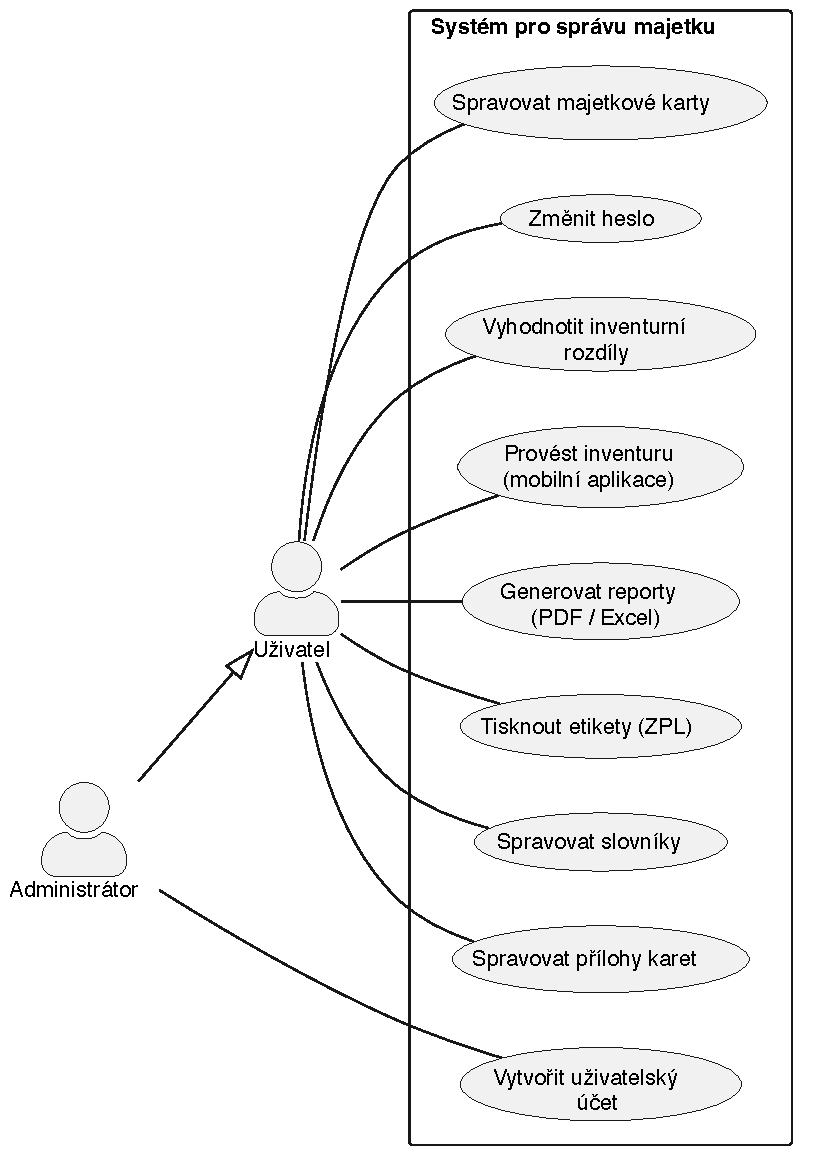
\includegraphics[width=0.65\textwidth]{images/use-case-diagram.pdf}
	\caption{Diagram případů užití}\label{fig:use-case-diagram}
\end{figure}

Diagram případů užití je znázorněn na obrázku~\ref{fig:use-case-diagram}. Následující podsekce popisují klíčové scénáře. U~všech scénářů se předpokládá, že uživatel je přihlášen.

\subsection{Správa majetkové karty}

\textbf{Cíl:} Vytvořit, upravit nebo duplikovat majetkovou kartu v~evidenci.

\begin{enumerate}
	\item Systém zobrazí seznam majetkových karet v~levém panelu.
	\item Uživatel klikne na tlačítko pro vytvoření nové karty.
	\item Systém zobrazí formulář s~povinnými poli (název, umístění, skupina, datum pořízení) a~volitelnými poli.
	\item Uživatel vyplní údaje a~potvrdí uložení.
	\item Systém ověří správnost zadaných dat (povinná pole, formáty) a~vytvoří kartu.
\end{enumerate}

\textit{Alternativní scénář:} Uživatel vybere existující kartu ze~seznamu, upraví její atributy a~uloží změny. Pro rychlé zadávání podobného majetku může existující kartu duplikovat.

\subsection{Tisk etiket}

\textbf{Cíl:} Vytisknout etikety s~Data Matrix kódy pro vybrané karty majetku nebo místnosti.

\begin{enumerate}
	\item Uživatel vyhledá požadované karty pomocí fulltextového vyhledávání nebo filtrů a~klikne na tlačítko tisku.
	\item Systém vygeneruje ZPL etikety a~odešle je na tiskárnu Zebra prostřednictvím cloudového tisku, případně nabídne ke~stažení jako \texttt{.zpl} soubor pro lokální tisk.
	\item Uživatel nalepí vytištěné etikety na příslušné položky majetku. Etikety místností se lepí na zárubně dveří.
\end{enumerate}

\subsection{Sběr inventurních dat}

\textbf{Cíl:} Zaznamenat skutečné umístění majetku v~terénu pomocí mobilní aplikace.

\begin{enumerate}
	\item Pracovník vyžádá stažení aktuálních dat ze~serveru.
	\item Systém ověří připojení, autentizuje se vůči serveru a~uloží karty a~lokace do~lokální databáze.
	\item Pracovník naskenuje Data Matrix kód místnosti.
	\item Systém nastaví aktuální umístění a~zobrazí jeho název.
	\item Pracovník postupně skenuje kódy majetku v~dané místnosti.
	\item U~každé naskenované karty systém barevně signalizuje, zda karta evidenčně patří do~aktuálního umístění (zelená), jiného umístění (oranžová), nebo nebyla v~databázi nalezena (červená), a~ukládá záznam o~naskenování do~lokální databáze.
	\item Po dokončení místnosti pracovník přejde do~další a~opakuje kroky 3--6.
	\item Pracovník vyžádá nahrání inventurních dat na server.
	\item Systém odešle všechny lokální záznamy hromadným požadavkem a~potvrdí úspěch.
\end{enumerate}

\subsection{Vyhodnocení inventury}

\textbf{Cíl:} Porovnat evidovaný stav majetku se skutečným a~promítnout změny do~databáze.

\begin{enumerate}
	\item Systém zobrazí seznam všech karet s~barevným rozlišením:
	\begin{itemize}
		\item \textit{Shodné} (zelená) -- evidované umístění odpovídá skutečnosti.
		\item \textit{Upozornění} (oranžová) -- karta nalezena na jiném umístění.
		\item \textit{Chybné} (červená) -- karta nebyla při inventuře naskenována.
	\end{itemize}
	\item U~karet se~stavem \uv{upozornění} uživatel zvolí: přijmout skutečné umístění, ponechat evidované, nebo majetek vyřadit. U~karet se~stavem \uv{chybné} lze ponechat evidované umístění nebo majetek vyřadit. U~shodných karet lze rovněž zvolit vyřazení.
	\item Po rozhodnutí u~všech karet s~nesouladem uživatel potvrdí promítnutí změn.
	\item Systém ověří, že každá karta se~stavem \uv{chybné} má zvolenou akci a~každá vyřazovaná karta má vyplněné datum a~způsob vyřazení. Poté aplikuje změny do~databáze.
\end{enumerate}

\subsection{Generování reportů}

\textbf{Cíl:} Vygenerovat přehledovou sestavu majetku pro potřeby účetnictví.

\begin{enumerate}
	\item Uživatel zvolí typ sestavy (podle skupiny majetku, podle místnosti, nebo pro konkrétní kartu).
	\item Uživatel vyplní parametry sestavy:
		\begin{itemize}
			\item \textit{podle skupiny majetku} -- konkrétní skupinu (nebo všechny skupiny) a~rozhodný den, ke~kterému se sestava generuje;
			\item \textit{podle místnosti} -- konkrétní místnost (číselník umístění);
			\item \textit{pro konkrétní kartu} -- identifikátor karty.
		\end{itemize}
	\item Systém vygeneruje PDF dokument a~zobrazí jej přímo v~prohlížeči.
	\item Uživatel si může sestavu stáhnout nebo vytisknout.
\end{enumerate}

\medskip

Vazba mezi případy užití a~funkčními požadavky je shrnuta v~tabulce~\ref{tab:uc-fr-mapping}.

\begin{table}[H]\centering
\renewcommand{\arraystretch}{1.3}
\caption{Mapování případů užití na funkční požadavky}\label{tab:uc-fr-mapping}
\begin{tabular}{l|l}
	\textbf{Případ užití} & \textbf{Plněné funkční požadavky} \tabularnewline \hline
	Správa majetkové karty & F-01 -- F-07 \tabularnewline
	Tisk etiket            & F-09 -- F-11 \tabularnewline
	Sběr inventurních dat  & F-16 -- F-20 \tabularnewline
	Vyhodnocení inventury  & F-21 -- F-24 \tabularnewline
	Generování reportů     & F-12 -- F-15 \tabularnewline
\end{tabular}
\end{table}



\chapter{Volba technologií}\label{chap:technologies}

\begin{chapterabstract}
	Tato kapitola srovnává technologie a~frameworky vhodné pro implementaci jednotlivých částí aplikace. Pro každou vrstvu (backend, frontend, mobilní aplikace) jsou porovnány dostupné alternativy s~vyhodnocením výhod a~nevýhod. Kapitola je zakončena přehledem dalších klíčových knihoven použitých v~projektu.
\end{chapterabstract}

Vyvíjený systém se skládá ze tří hlavních komponent: serverové části (backend), webové aplikace (frontend) a~mobilní aplikace pro inventuru (Android). Každá z~těchto komponent vyžaduje volbu vhodné technologie, přičemž je nutné zohlednit vzájemnou kompatibilitu a~dostupnost knihoven. Všechny zvažované technologie jsou open-source a~bezplatné. Při volbě byla zohledněna i~předchozí zkušenost autora, která umožnila efektivní vývoj.

\section{Backend}

Backend aplikace zajišťuje veškerou business logiku, komunikaci s~databází, autentizaci uživatelů a~generování exportů. Jedná se o~REST API, které obsluhuje jak webovou aplikaci, tak mobilní aplikaci. Pro jeho implementaci byly zvažovány tři technologie.

\subsection{Spring Boot (Java)}

Spring Boot je framework postavený nad platformou Spring, který podle oficiální dokumentace \uv{pomáhá vytvářet samostatné, produkčně kvalitní aplikace založené na Springu s~minimálním úsilím} (překlad vlastní)~\cite{springboot}. Framework zastává tzv. opinionated přístup -- poskytuje rozumné výchozí konfigurace, které lze v~případě potřeby přepsat.

Mezi hlavní přednosti Spring Boot patří rozsáhlý ekosystém. Spring Data JPA~\cite{springdatajpa} nabízí abstrakci nad databázovou vrstvou pomocí Jakarta Persistence API, Spring Security~\cite{springsecurity} poskytuje komplexní řešení autentizace a~autorizace včetně podpory JWT tokenů a~OAuth2. Framework dále disponuje vestavěným webovým serverem (Tomcat), automatickou konfigurací na základě přítomných závislostí a~robustní podporou pro testování prostřednictvím JUnit~5 a~Mockito.

Nevýhodou Spring Boot je vyšší paměťová náročnost typická pro aplikace běžící na JVM a~delší doba studeného startu oproti interpretovaným jazykům. Pro aplikace s~nízkou frekvencí změn v~nasazení, jako je tento projekt, však tato nevýhoda není podstatná.

\subsection{NestJS (TypeScript)}

NestJS~\cite{nestjs} je Node.js framework nabízející modulární architekturu inspirovanou Angularem, vestavěný systém Dependency Injection a~podporu TypeScriptu jako prvotřídního jazyka. Je postaven nad minimalistickým Express.js~\cite{expressjs}, ale na rozdíl od něj poskytuje kompletní strukturu aplikace. Pro práci s~databází lze využít TypeORM nebo Prisma.

Hlavní výhodou je možnost sdílení TypeScriptových typů mezi backendem a~frontendem. Pro tento projekt je nevýhodou absence knihoven srovnatelných s~iText (generování PDF) a~EasyExcel (export do XLSX) v~ekosystému Node.js -- dostupné alternativy (např.\ PDFKit, ExcelJS) nenabízejí stejnou úroveň podpory pro složitější tabulkové reporty a~lokalizaci.

\subsection{Django (Python)}

Django~\cite{django} je plnohodnotný webový framework pro Python, zastávající filozofii \uv{batteries included} -- součástí je vestavěný ORM, administrační rozhraní, systém autentizace i~ochrana proti běžným bezpečnostním hrozbám (CSRF, SQL injection).

Automaticky generované administrační rozhraní je výhodou pro projekty vyžadující rychlý prototyping. Nevýhodou Djanga je dynamický typový systém Pythonu, který oproti Javě nenabízí statickou kontrolu typů v~době kompilace, což může vést k~obtížněji odhalitelným chybám. Ekosystém knihoven pro generování PDF a~ZPL etiket je v~Pythonu rovněž méně rozvinutý než v~prostředí JVM.

\subsection{Srovnání a~zdůvodnění volby}

Tabulka~\ref{tab:backend-comparison} shrnuje srovnání analyzovaných backend technologií.

\begin{table}[htbp]\centering\footnotesize
\begin{tabular}{l|c|c|c}
	\textbf{Kritérium} & \textbf{Spring Boot} & \textbf{NestJS} & \textbf{Django} \tabularnewline \hline
	Jazyk & Java & TypeScript & Python \tabularnewline
	Typová bezpečnost & silná & silná & dynamická \tabularnewline
	ORM & JPA (Hibernate) & TypeORM / Prisma & vlastní ORM \tabularnewline
	Bezpečnostní framework & Spring Security & Passport.js & vestavěný \tabularnewline
	Podpora PDF/Excel/ZPL & iText, EasyExcel & omezená & omezená \tabularnewline
\end{tabular}
\caption{Srovnání backend technologií}\label{tab:backend-comparison}
\end{table}

Pro implementaci backendu byl zvolen \textbf{Spring Boot} z~následujících důvodů:
\begin{itemize}
	\item Robustní ekosystém pro enterprise aplikace -- Spring Data JPA pro databázovou vrstvu, Spring Security pro autentizaci a~autorizaci.
	\item Dostupnost kvalitních knihoven pro generování PDF (iText), Excelu (EasyExcel) a~ZPL etiket -- klíčová funkčnost pro tento projekt.
	\item Silná typová bezpečnost jazyka Java, která usnadňuje údržbu a~refaktoring.
	\item Konzistence s~mobilní aplikací, která je rovněž implementována v~Javě.
\end{itemize}


\section{Frontend}

Webová aplikace slouží jako hlavní rozhraní pro správu majetkových karet, číselníků, uživatelů a~vyhodnocení inventurních dat. Jedná se o~jednostránkovou aplikaci (SPA) komunikující s~backendem prostřednictvím REST API. Pro její implementaci byly zvažovány tři přední JavaScriptové technologie.

\subsection{React}

React je podle své dokumentace \uv{knihovna pro tvorbu webových a~nativních uživatelských rozhraní} (překlad vlastní)~\cite{react}. Na rozdíl od Angularu se nejedná o~kompletní framework, ale o~knihovnu zaměřenou výhradně na vrstvu uživatelského rozhraní. Výběr ostatních nástrojů (routing, state management, formuláře) je ponechán na vývojáři.

React využívá komponentovou architekturu a~deklarativní přístup prostřednictvím JSX syntaxe. Systém Hooks (\texttt{useState}, \texttt{useEffect}) umožňuje správu stavu a~vedlejších efektů ve funkcionálních komponentách. Ekosystém Reactu je největší ze srovnávaných technologií -- zahrnuje knihovny jako MUI~\cite{mui} pro komponentové UI, TanStack Query~\cite{tanstackquery} pro správu serverového stavu, React Hook Form~\cite{reacthookform} pro formuláře či Zustand~\cite{zustand} pro globální stav.

Nevýhodou Reactu je nutnost skládat aplikaci z~mnoha nezávislých knihoven, což vyžaduje zkušenost s~výběrem a~integrací těchto nástrojů.

\subsection{Angular}

Angular~\cite{angular} je plnohodnotný, opinionated framework vyvíjený týmem ve společnosti Google. Angular poskytuje kompletní sadu nástrojů přímo v~základním balíčku -- vlastní router, HTTP klient, systém formulářů, Dependency Injection a~build toolchain.

TypeScript je v~Angularu povinný, což zajišťuje silnou typovou bezpečnost. Framework dále nabízí reaktivní systém Angular Signals a~vestavěnou podporu pro Server-Side Rendering. Nevýhodou je strmější křivka učení a~větší režie pro menší projekty, kde plnohodnotný framework může být zbytečně komplexní.

\subsection{Vue.js}

Vue.js~\cite{vuejs} je progresivní framework navržený s~důrazem na inkrementální adoptovatelnost -- lze jej použít jak jako jednoduchou knihovnu pro obohacení existujících stránek, tak jako základ pro plnohodnotnou SPA.

Vue nabízí dvě API rozhraní: Options API (přívětivější pro začátečníky) a~Composition API (doporučené pro větší aplikace). Ekosystém obsahuje oficiální řešení pro routing (Vue Router) a~state management (Pinia). Oproti Reactu je ekosystém UI knihoven menší, i~když dostupné jsou například Vuetify nebo Quasar.

\subsection{Srovnání a~zdůvodnění volby}

Tabulka~\ref{tab:frontend-comparison} shrnuje srovnání analyzovaných frontend technologií.

\begin{table}[htbp]\centering\footnotesize
\begin{tabular}{l|c|c|c}
	\textbf{Kritérium} & \textbf{React} & \textbf{Angular} & \textbf{Vue.js} \tabularnewline \hline
	Typ & knihovna & framework & framework \tabularnewline
	TypeScript & volitelný & povinný & volitelný \tabularnewline
	State management & Zustand, Redux & Signals, NgRx & Pinia \tabularnewline
	UI knihovny & MUI, shadcn & Angular Material & Vuetify, Quasar \tabularnewline
	Přístup & neopinionated & opinionated & progresivní \tabularnewline
\end{tabular}
\caption{Srovnání frontend technologií}\label{tab:frontend-comparison}
\end{table}

Pro implementaci frontendu byla zvolena knihovna \textbf{React} společně s~jazykem
\textbf{TypeScript}~\cite{typescript} z~následujících důvodů:
\begin{itemize}
	\item Největší ekosystém UI knihoven -- MUI~\cite{mui} poskytuje hotové komponenty odpovídající Material Design, včetně tabulek, dialogů a~formulářových prvků potřebných pro správu dat.
	\item Flexibilita při výběru knihoven -- možnost zvolit optimální nástroj pro každou oblast (TanStack Query pro data fetching, React Hook Form + Zod pro formuláře, Zustand pro globální stav).
\end{itemize}

Jako build nástroj byl zvolen \textbf{Vite}~\cite{vite}, který nabízí rychlý vývojový server s~Hot Module Replacement a~optimalizovaný produkční build.


\section{Mobilní aplikace}

Mobilní aplikace slouží k~provádění inventury v~terénu -- pracovník skenuje Data Matrix kódy na majetku pomocí čtečky Zebra TC22 a~zaznamenává skutečné umístění položek. Aplikace pracuje offline a~data synchronizuje se serverem, jakmile je dostupné připojení k~síti. Cílovým zařízením je výhradně Android.

\subsection{Nativní Android (Java)}

Nativní vývoj pro Android~\cite{android} v~jazyce Java poskytuje přímý přístup ke všem API platformy bez jakékoliv abstrakční vrstvy. Pro lokální ukládání dat je k~dispozici knihovna Room~\cite{androidroom}, která podle oficiální dokumentace \uv{poskytuje abstrakční vrstvu nad SQLite umožňující plynulý přístup k~databázi při využití plného potenciálu SQLite} (překlad vlastní). Room ověřuje SQL dotazy v~době kompilace a~minimalizuje boilerplate kód prostřednictvím anotací.

Pro HTTP komunikaci lze využít knihovnu OkHttp~\cite{okhttp}, která podporuje synchronní i~asynchronní požadavky. Hlavní výhodou nativního přístupu je plná kontrola nad lifecycle komponent a~přímá kompatibilita se vstupem z~hardwarového skeneru, který posílá data jako klávesnicové události.

Nevýhodou je omezení na jedinou platformu a~větší množství boilerplate kódu oproti modernějším alternativám.

\subsection{Kotlin}

Kotlin~\cite{kotlin} je oficiálně doporučený jazyk pro vývoj Android aplikací. Nabízí modernější syntaxi než Java -- \texttt{null} safety na úrovni typového systému, korutiny pro asynchronní programování a~méně boilerplate kódu. Kotlin je plně interoperabilní s~Javou, což umožňuje postupnou migraci existujícího kódu.

Pro tento projekt by Kotlin nepřinesl zásadní výhody. Aplikace je architektonicky jednoduchá (jedna Activity, tři fragmenty) a~nevyužívá složité asynchronní vzory, pro které jsou korutiny navrženy. Zavedení dalšího jazyka do projektu by zvýšilo komplexitu bez odpovídajícího přínosu.

\subsection{Flutter / React Native}

Flutter~\cite{flutter} je multiplatformní framework od Google, který používá jazyk Dart a~vlastní vykreslovací engine obcházející nativní UI komponenty platformy. React Native~\cite{reactnative} vykresluje JavaScriptový kód prostřednictvím nativních komponent; doporučeným meta-frameworkem je Expo.

Obě technologie nabízejí multiplatformní vývoj, který však v~tomto projektu není potřeba -- cílovým zařízením je výhradně Zebra TC22 se systémem Android. Zásadním problémem je omezená podpora specifického hardwaru: vstup ze skeneru přichází jako události hardwarové klávesnice zakončené klávesou Enter nebo Tab, což vyžaduje přímý přístup k~nativním listenerům (\texttt{OnKeyListener}, \texttt{OnEditorActionListener}). Abstrakční vrstva multiplatformních frameworků by tento přístup komplikovala.

\subsection{Srovnání a~zdůvodnění volby}

Tabulka~\ref{tab:mobile-comparison} shrnuje srovnání analyzovaných mobilních technologií.

\begin{table}[htbp]\centering\footnotesize
\begin{tabular}{l|c|c|c}
	\textbf{Kritérium} & \textbf{Java (nativní)} & \textbf{Kotlin} & \textbf{Flutter / RN} \tabularnewline \hline
	Platformy & Android & Android (+ KMP) & Android + iOS \tabularnewline
	Přístup k~HW skeneru & přímý & přímý & přes bridge \tabularnewline
	Offline DB & Room (SQLite) & Room (SQLite) & SQLite plugin \tabularnewline
	Složitost & nízká & nízká & střední \tabularnewline
\end{tabular}
\caption{Srovnání mobilních technologií}\label{tab:mobile-comparison}
\end{table}

Pro implementaci mobilní aplikace byl zvolen \textbf{nativní Android v~Javě} z~následujících důvodů:
\begin{itemize}
	\item Přímý přístup k~hardwarovému skeneru Zebra -- vstup přichází jako klávesnicové události, které je nutné zpracovat prostřednictvím nativních listenerů.
	\item Plná kontrola nad lifecycle komponent -- aplikace pracuje offline s~lokální Room databází a~vyžaduje přesnou správu synchronizace dat.
	\item Jednoduchost -- pro aplikaci s~jednou Activity a~třemi fragmenty není potřeba složitý framework.
	\item Konzistence s~backendem -- oba projekty sdílejí jazyk Java, což usnadňuje přechod mezi jednotlivými částmi projektu.
\end{itemize}


\section{Databázový systém}

Systém využívá relační databázi pro ukládání majetkových karet, číselníků, uživatelů a~inventurních záznamů. Na mobilním zařízení je navíc potřeba lokální databáze pro offline režim. Pro produkční nasazení byly zvažovány dva databázové systémy.

\subsection{PostgreSQL}

PostgreSQL~\cite{postgresql} je objektově-relační databázový systém s~více než 35 lety aktivního vývoje. Nabízí podporu komplexních datových typů (JSONB, pole), fulltextové vyhledávání, rozšiřitelnost prostřednictvím vlastních funkcí (např.\ \texttt{unaccent} pro vyhledávání bez diakritiky) a~vysokou spolehlivost.

\subsection{MySQL / MariaDB}

MySQL~\cite{mysql} je nejrozšířenější open-source relační databáze s~širokou podporou u~hostingových poskytovatelů. MariaDB~\cite{mariadb} je komunitní fork MySQL se zpětnou kompatibilitou, který MySQL v~open-source prostředí postupně nahrazuje. Pro účely tohoto projektu by oba systémy poskytovaly dostatečnou funkčnost. PostgreSQL byl zvolen díky podpoře funkce \texttt{unaccent} pro vyhledávání bez diakritiky a~předchozí zkušenosti autora.

\subsection{H2 a~Room}

Pro automatizované testování backendu byla zvolena in-memory databáze \textbf{H2}~\cite{h2database} v~PostgreSQL compatibility mode. H2 je kompatibilní s~JPA a~nevyžaduje žádnou externí infrastrukturu, testy tak běží izolovaně a~reproducibilně. Testy ověřují business logiku a~JPA dotazy; SQL specifika PostgreSQL (např.\ funkce \texttt{unaccent}) jsou testována prostřednictvím integračních testů.

Na mobilním zařízení je využita knihovna \textbf{Room}~\cite{androidroom} jako abstrakce nad SQLite. Room poskytuje ověřování SQL dotazů v~době kompilace, automatické mapování mezi Java objekty a~databázovými tabulkami prostřednictvím anotací (\texttt{@Entity}, \texttt{@Dao}, \texttt{@Query}) a~podporu migrací.

\subsection{Zdůvodnění volby}

Pro produkční nasazení byl zvolen \textbf{PostgreSQL} díky zralosti, spolehlivosti a~výborné integraci se Spring Data JPA. Všechny zvažované databázové systémy jsou open-source a~bezplatné, takže náklady na licence nebyly rozhodovacím faktorem. Kombinace PostgreSQL (produkce), H2 (testy) a~Room/SQLite (mobilní zařízení) pokrývá potřeby všech tří prostředí.


\section{Další klíčové knihovny}

Kromě hlavních technologií popsaných výše projekt využívá řadu specializovaných knihoven, které výrazně zefektivňují vývoj.

\subsection{Backend knihovny}

\textbf{MapStruct}~\cite{mapstruct} je generátor kódu pro mapování mezi Java beany (typicky DTO a~entity). Na rozdíl od reflexe-based řešení generuje mapovací kód v~době kompilace, což zajišťuje typovou bezpečnost a~vyšší výkon.

\textbf{Project Lombok}~\cite{lombok} redukuje boilerplate kód prostřednictvím anotací~-- \texttt{@Getter}, \texttt{@Setter} a~\texttt{@RequiredArgsConstructor} generují gettery, settery a~konstruktory automaticky. Lombok je nakonfigurován tak, aby generovaný kód byl označen anotací \texttt{@Generated}, čímž je vyloučen z~měření pokrytí kódu testy.

\subsection{Frontend knihovny}

\textbf{TanStack Query}~\cite{tanstackquery} zajišťuje správu serverového stavu -- automatické cachování, invalidaci a~refetching dat z~API. Všechna data ve webové aplikaci jsou načítána výhradně prostřednictvím TanStack Query hooků.

\textbf{React Hook Form}~\cite{reacthookform} v~kombinaci s~validační knihovnou \textbf{Zod}~\cite{zod} zajišťuje správu formulářů s~typově bezpečnou validací. Validační schémata definovaná v~Zod slouží zároveň jako dokumentace očekávaného formátu dat.

\textbf{Zustand}~\cite{zustand} je minimalistická knihovna pro globální state management, využitá pro správu autentizačního stavu (uživatel, JWT token, expirace).

\textbf{MUI}~\cite{mui} (Material UI) poskytuje hotové React komponenty implementující Material Design -- tabulky, dialogová okna, formulářové prvky a~navigaci. Díky MUI bylo možné rychle vytvořit konzistentní a~přístupné uživatelské rozhraní.



\chapter{Návrh architektury}\label{chap:architecture}

\begin{chapterabstract}
	Kapitola popisuje celkovou architekturu systému, návrh jednotlivých komponent a~datový model. Nejprve je představen přehled systému a~komunikace mezi jeho částmi, následně je podrobně popsána architektura backendu, frontendu a~mobilní aplikace.
\end{chapterabstract}

\section{Přehled systému}

Systém se skládá ze tří hlavních komponent, které spolu komunikují prostřednictvím REST API přes protokol HTTPS (viz obrázek~\ref{fig:system-architecture}):

\begin{itemize}
	\item \textbf{Backend} -- serverová aplikace (Spring Boot) poskytující REST API, business logiku, generování exportů a~přístup k~databázi PostgreSQL. Backend je nasazen na linuxovém VPS serveru za reverse proxy Nginx.
	\item \textbf{Frontend} -- jednostránková webová aplikace (React) pro správu majetku, uživatelů a~vyhodnocení inventury. Komunikuje výhradně s~backendem prostřednictvím REST API.
	\item \textbf{Mobilní aplikace} -- nativní Android aplikace pro inventuru v~terénu. Disponuje vlastní lokální databází (Room/SQLite) pro offline režim a~se serverem se synchronizuje na vyžádání.
\end{itemize}

\begin{figure}[H]\centering
	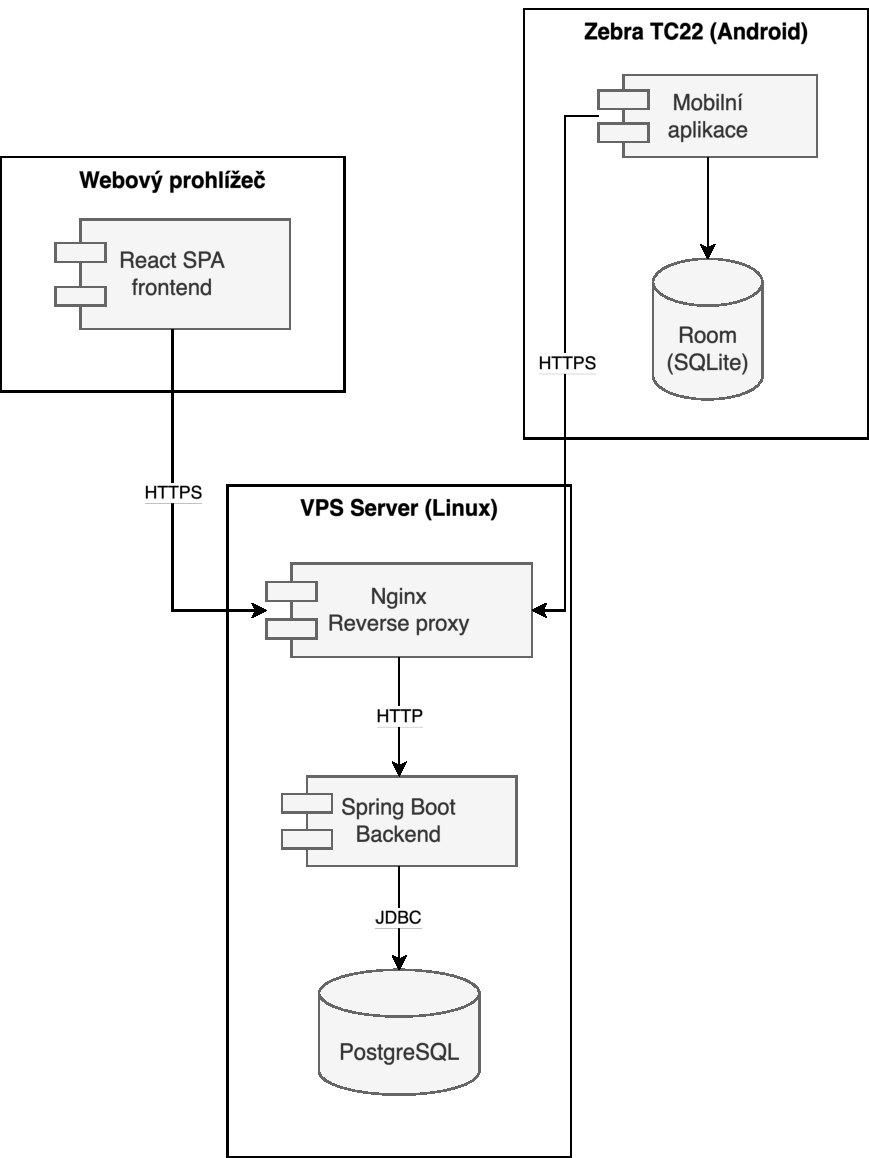
\includegraphics[width=0.85\textwidth]{images/system-architecture.pdf}
	\caption{Diagram architektury systému}\label{fig:system-architecture}
\end{figure}

Frontend ani mobilní aplikace spolu přímo nekomunikují -- veškerá výměna dat probíhá prostřednictvím backendu. Tento přístup centralizuje business logiku a~zjednodušuje bezpečnostní model, neboť autentizace a~autorizace jsou řešeny na jednom místě.

\section{Architektura backendu}\label{sec:backend-arch}

Backend je organizován jako modulární monolitická aplikace -- každá doménová oblast (karty majetku, autentizace, číselníky, inventurní audit, přílohy) má vlastní balíček obsahující celý vertikální řez od kontroleru po repozitář. Tento přístup byl zvolen oproti klasickému vrstvovému uspořádání (všechny kontrolery v~jednom balíčku, všechny služby v~druhém), protože drží související kód pohromadě a~usnadňuje orientaci v~projektu -- při práci na konkrétní funkčnosti není nutné přecházet mezi vzdálenými částmi stromu zdrojových souborů.

\subsection{Vrstvená architektura}

Každý modul dodržuje konzistentní třívrstvý vzor odpovídající klasické enterprise architektuře~\cite{fowler-eaa}:

\begin{enumerate}
	\item \textbf{Controller} (\texttt{@RestController}) -- přijímá HTTP požadavky, provádí vstupní validaci prostřednictvím anotace \texttt{@Valid} a~deleguje zpracování na service vrstvu. Vrací \texttt{ResponseEntity} s~příslušným HTTP kódem.
	\item \textbf{Service} -- definovaný jako rozhraní (\texttt{IXxxService}) s~implementací v~podbalíčku \texttt{implementation}. Oddělení rozhraní od implementace je běžný vzor ve Spring ekosystému -- dodržuje SOLID princip Dependency Inversion, usnadňuje mockování v~unit testech a~zjednodušuje případné rozšíření o~alternativní implementaci. Service obsahuje business logiku a~řídí transakce prostřednictvím anotace \texttt{@Transactional}.
	\item \textbf{Repository} -- rozhraní rozšiřující \texttt{JpaRepository}, které poskytuje přístup k~databázi. Dotazy jsou buď odvozeny z~názvu metody, nebo definovány explicitně anotací \texttt{@Query}.
\end{enumerate}

Mezi vrstvami je zajištěna separace dat prostřednictvím vzoru DTO (Data Transfer Object)~\cite{fowler-eaa}. Mapování mezi entitami a~DTO zajišťuje knihovna MapStruct, která generuje mapovací kód v~době kompilace. Kontrolery nikdy nepracují přímo s~JPA entitami -- vždy přijímají a~vracejí DTO objekty.

\subsection{Modulární struktura}

Backend je rozdělen do následujících modulů:

\begin{itemize}
	\item \textbf{auth} -- autentizace, správa uživatelů, bezpečnostní konfigurace (JWT filtry, Spring Security)
	\item \textbf{card} -- CRUD operace nad kartami majetku, filtrování, generování exportů (PDF, Excel, ZPL)
	\item \textbf{attachment} -- správa souborových příloh ke~kartám majetku
	\item \textbf{inventoryaudit} -- import inventurních dat z~mobilní aplikace, výpočet rozdílů, projekce změn
	\item \textbf{dictionary} -- pět číselníkových podmodulů (umístění, skupiny, třídy, způsoby pořízení, způsoby vyřazení), každý se shodnou strukturou
	\item \textbf{entity} -- centralizované JPA entity sdílené napříč moduly
	\item \textbf{exception} -- globální zpracování výjimek (\texttt{@RestControllerAdvice}). Doménové výjimky jsou převedeny na strukturované JSON odpovědi s~příslušným HTTP kódem. Na frontendu jsou chyby zobrazeny toast notifikacemi, v~mobilní aplikaci barevně odlišenými stavovými zprávami.
	\item \textbf{config} -- konfigurace aplikace (OpenAPI dokumentace, kódování hesel)
\end{itemize}

Struktura balíčků je znázorněna na obrázku~\ref{fig:package-backend}. Všechny doménové moduly závisí na balíčku \texttt{entity}, který obsahuje sdílené JPA entity.

\begin{figure}[H]\centering
	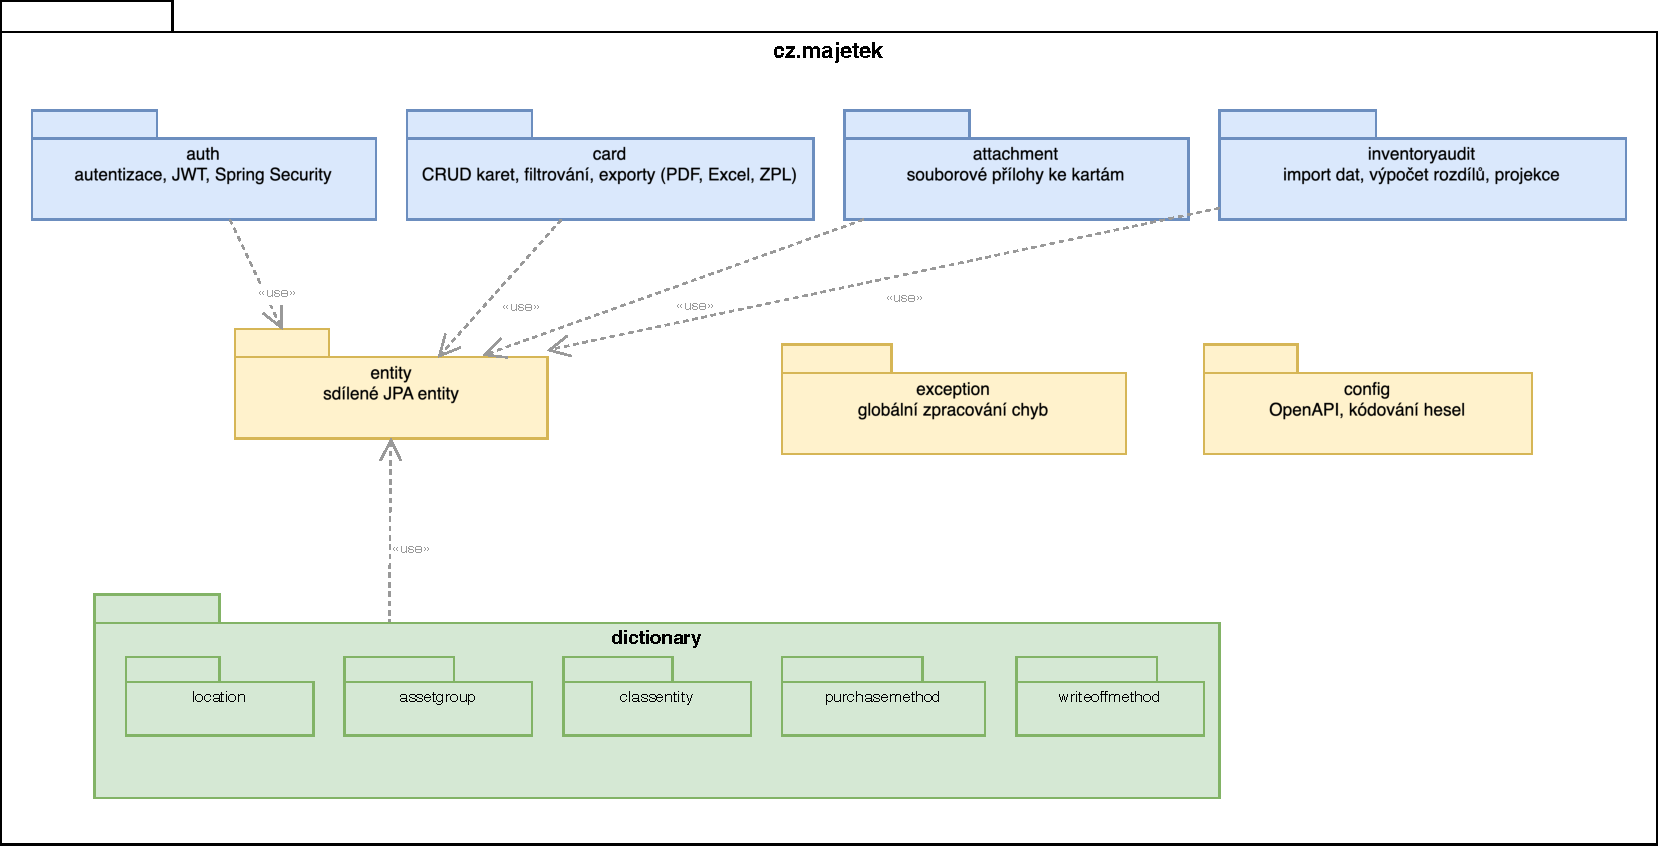
\includegraphics[width=\textwidth]{images/package-backend.pdf}
	\caption{Diagram balíčků backendu}\label{fig:package-backend}
\end{figure}

\subsection{Bezpečnostní model}

Autentizace je realizována pomocí JSON Web Tokenů (JWT)~\cite{jwt}. Systém využívá dvě samostatné bezpečnostní filter chains v~rámci Spring Security:

\begin{enumerate}
	\item \textbf{Basic Auth chain} -- zachytává výhradně požadavek na přihlášení (\texttt{POST /api/auth/login}). Po ověření přihlašovacích údajů vygeneruje access token (krátká platnost) a~refresh token (delší platnost).
	\item \textbf{JWT Bearer chain} -- zachytává všechny ostatní API požadavky. Filtr \texttt{JwtAuthenticationFilter} extrahuje token z~hlavičky \texttt{Authorization: Bearer}, ověří jeho platnost a~nastaví bezpečnostní kontext.
\end{enumerate}

Access token je přenášen v~HTTP hlavičce, refresh token výhradně v~\texttt{httpOnly} cookie s~příznakem \texttt{Secure} a~\texttt{SameSite=Strict}. Při obnovení (endpoint \texttt{/api/\allowbreak auth/\allowbreak refresh}) server ověří platnost refresh tokenu, zkontroluje jeho jedinečný identifikátor (\texttt{jti}) oproti hodnotě uložené v~databázi a~vygeneruje nový pár tokenů. Starý refresh token je tímto invalidován -- jedná se o~tzv.\ rotaci tokenů, která prodlužuje session při aktivním používání a~zároveň zajišťuje, že kompromitovaný token nelze opakovaně použít. Celý autentizační tok je znázorněn na obrázku~\ref{fig:jwt-auth-flow}.

\begin{figure}[H]\centering
	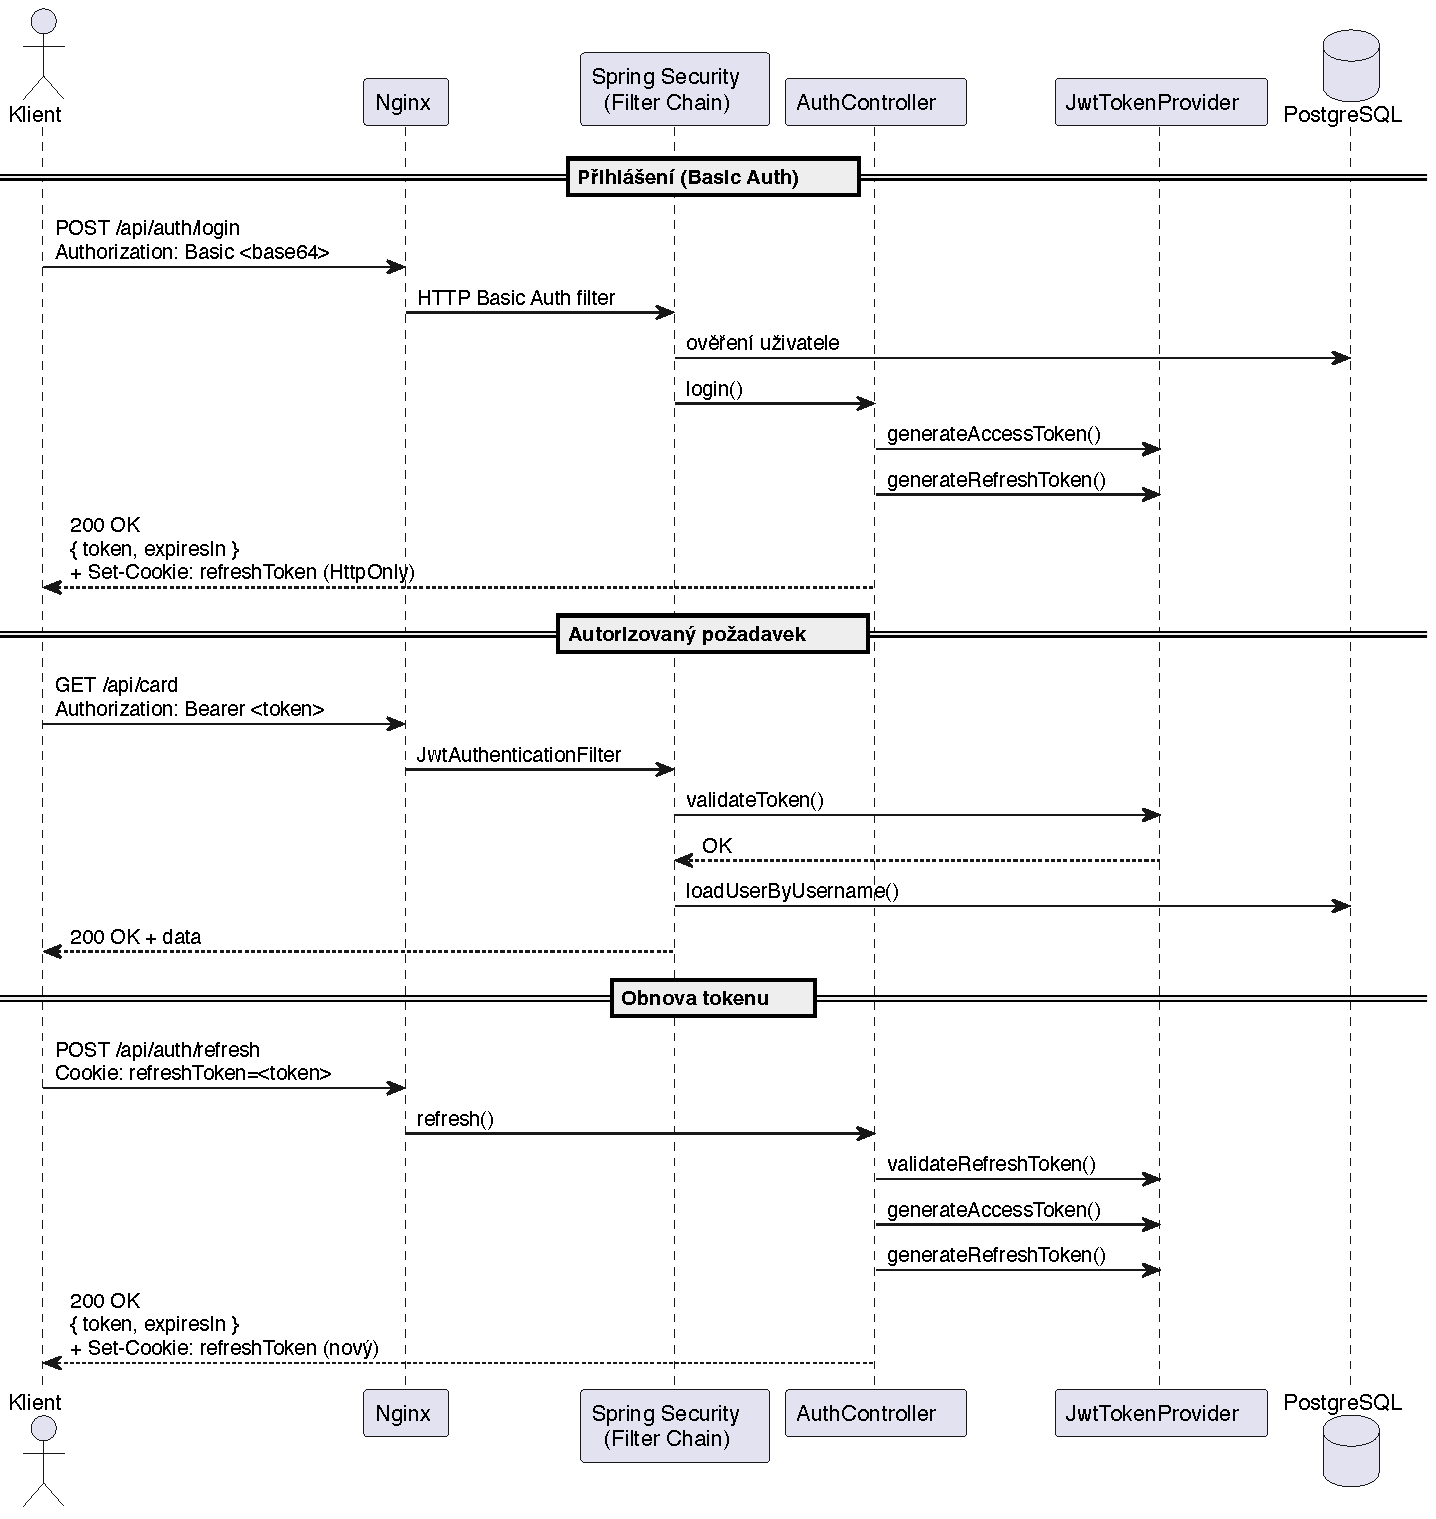
\includegraphics[width=\textwidth]{images/jwt-auth-flow.pdf}
	\caption{Sekvenční diagram autentizačního flow}\label{fig:jwt-auth-flow}
\end{figure}

Autorizace rozlišuje dvě role: \texttt{USER} a~\texttt{ADMIN}. Jediným endpointem omezeným na roli administrátora je registrace nového uživatele, chráněná anotací \texttt{@PreAuthorize}. Ostatní endpointy vyžadují pouze platný JWT token bez ohledu na roli.

\section{Architektura frontendu}

Frontend je jednostránková aplikace (SPA) v~Reactu a~TypeScriptu. Architektura je navržena s~důrazem na oddělení zodpovědností.

\subsection{Vrstvená architektura}

\begin{enumerate}
	\item \textbf{Services} (\texttt{services/}) -- čisté asynchronní funkce pro komunikaci s~API prostřednictvím knihovny Axios. Každá doménová entita má vlastní service soubor. Funkce transformují data z~API formátu do TypeScriptových typů.
	\item \textbf{Query hooks} (\texttt{hooks/queries/}) -- wrappery nad TanStack Query, které zapouzdřují volání service funkcí. Query hooky zajišťují cachování, automatickou invalidaci a~správu serverového stavu.
	\item \textbf{Komponenty} (\texttt{components/}) -- znovupoužitelné UI komponenty organizované podle domény (card, dictionary, report, inventoryAudit).
	\item \textbf{Stránky} (\texttt{pages/}) -- komponenty na úrovni route, které skládají jednotlivé UI komponenty do celých obrazovek.
\end{enumerate}

\subsection{Správa stavu}

Webová aplikace pracuje se dvěma kategoricky odlišnými typy stavu, které vyžadují odlišné řešení. \textbf{Serverový stav} odpovídá datům uloženým v~databázi (karty majetku, číselníky, inventurní záznamy) -- aplikace si jeho aktuální podobu pouze cachuje a~musí řešit zastarávání cache, opětovné načtení po~mutaci a~konzistenci napříč obrazovkami. \textbf{Klientský stav} se naopak týká informací existujících pouze v~prohlížeči (přihlášený uživatel, otevřená modalní okna, lokální UI volby) a~vyžaduje synchronizaci pouze v~rámci jedné aplikační instance.

Vzhledem k~odlišné povaze obou typů stavu byly zvoleny dvě specializované knihovny:

\begin{itemize}
	\item \textbf{Serverový stav} je spravován knihovnou TanStack Query. Veškerá data z~API jsou cachována s~dobou platnosti dvě minuty. Mutace po úspěchu buď invalidují příslušné cache klíče (plný refetch), nebo optimisticky aktualizují cache přímo.
	\item \textbf{Klientský stav} je omezen na autentizační údaje (přihlášený uživatel, JWT token, expirace) a~spravuje jej jediný Zustand store. Axios interceptor automaticky obnovuje vypršelý token prostřednictvím refresh endpointu před odesláním požadavku.
\end{itemize}

Všechny chráněné stránky jsou obaleny komponentou \texttt{PrivateRoute}, která ověřuje přítomnost platného JWT tokenu v~Zustand store a~nepřihlášeného uživatele přesměruje na přihlašovací stránku. Chráněné stránky jsou načítány líně (\texttt{React.lazy}) -- jejich kód se stáhne až při prvním přístupu, což zkracuje počáteční dobu načtení.

\subsection{Generický vzor pro číselníky}

Pět číselníkových stránek sdílí generickou komponentu \texttt{DictionaryPage<T>}, parametrizovanou typem entity. Komponenta přijímá hooky pro query a~mutace jako vlastnosti a~vykresluje tabulku s~operacemi vytvoření, přejmenování a~smazání. Konkrétní stránky (např.\ \texttt{LocationPage}) jsou pouze wrappery, které předávají příslušné hooky a~volitelné rozšíření (např.\ tlačítko tisku etikety u~lokací).

\section{Architektura mobilní aplikace}\label{sec:mobile-arch}

Mobilní aplikace je navržena jako jednoduchá nativní Android aplikace s~jednou Activity a~třemi fragmenty. Architektura je přizpůsobena specifickým požadavkům -- offline režim, vstup z~hardwarového skeneru a~provoz na enterprise zařízení Zebra TC22.

\subsection{Struktura uživatelského rozhraní}

Aplikace využívá jednu \texttt{MainActivity}, která hostuje tři fragmenty přepínané prostřednictvím spodní navigační lišty (\texttt{BottomNavigationView}):

\begin{enumerate}
	\item \textbf{ControlScanFragment} -- kontrolní snímání. Umožňuje naskenovat kód majetku a~zobrazit jeho detail bez zápisu do inventury. Slouží pro rychlé ověření identity položky.
	\item \textbf{InventoryScanFragment} -- inventurní snímání. Dvoustupňový proces: nejprve se naskenuje kód místnosti (nastavení aktuálního umístění), poté se postupně skenují kódy majetku. Každé naskenování vytvoří záznam v~lokální databázi.
	\item \textbf{DataTransferFragment} -- přenos dat. Umožňuje stáhnout aktuální data ze~serveru, nahrát inventurní záznamy zpět a~konfigurovat URL serveru.
\end{enumerate}

\subsection{Offline režim a~synchronizace}

Mobilní aplikace využívá knihovnu Room jako abstrakci nad SQLite. Lokální databáze obsahuje tři tabulky: \texttt{card} (karty majetku), \texttt{location} (lokace) a~\texttt{inventory\_audit} (inventurní záznamy). Data karet a~lokací jsou stažena ze~serveru před zahájením inventury; inventurní záznamy vznikají lokálně při skenování. Tabulka \texttt{inventory\_audit} má primární klíč \texttt{card\_id} -- každá karta může mít nejvýše jeden inventurní záznam. Opakované naskenování téže karty aktualizuje existující záznam (strategie \texttt{REPLACE}).

Synchronizace probíhá výhradně na explicitní pokyn uživatele:

\begin{itemize}
	\item \textbf{Stažení dat} -- aplikace ověří připojení k~síti, autentizuje se prostřednictvím Basic Auth, stáhne aktuální karty a~lokace a~atomicky je uloží do lokální databáze v~rámci jedné transakce.
	\item \textbf{Odeslání inventury} -- aplikace načte všechny lokální inventurní záznamy, serializuje je do formátu JSON a~odešle hromadným požadavkem na server (\texttt{POST /api/inventory-audit/insert-many}).
\end{itemize}

Stažení nových dat je zablokováno, pokud v~lokální databázi existují neodeslaná inventurní data -- tím je zabráněno nechtěné ztrátě práce. Autentizační tokeny i~přihlašovací údaje jsou uloženy v~šifrovaném úložišti \texttt{EncryptedSharedPreferences} (AES-256-GCM). Síťová konfigurace zakazuje nešifrovanou komunikaci (\texttt{cleartext traffic}). Celý protokol synchronizace mezi mobilní aplikací, lokální Room databází a~serverem znázorňuje obrázek~\ref{fig:sequence-sync}.

\begin{figure}[H]\centering
	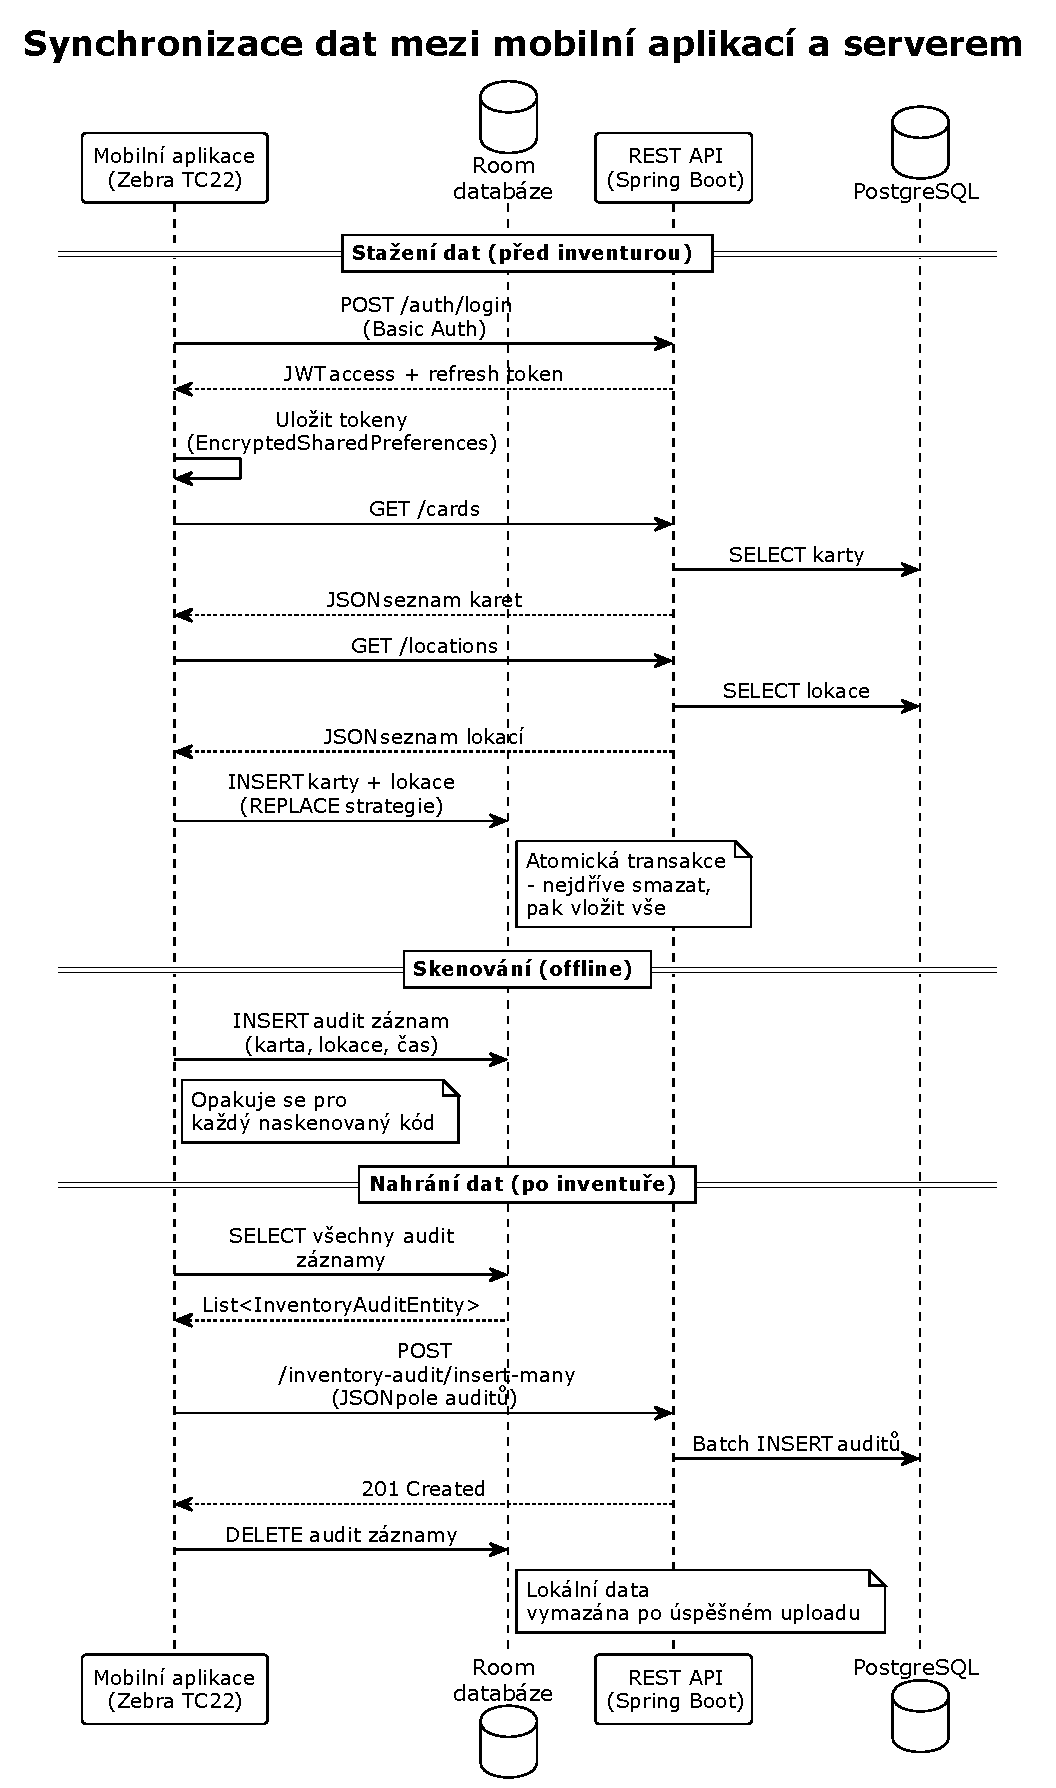
\includegraphics[width=\textwidth]{images/sequence-sync.pdf}
	\caption{Sekvenční diagram synchronizace dat mezi mobilní aplikací a~serverem}\label{fig:sequence-sync}
\end{figure}

\section{Datový model}

Datový model systému tvoří devět tabulek v~relační databázi PostgreSQL (viz obrázek~\ref{fig:er-diagram}). Centrální entitou je tabulka \texttt{card} (majetková karta), na~kterou se váží číselníkové tabulky, přílohy a~inventurní záznamy.

\begin{figure}[H]\centering
	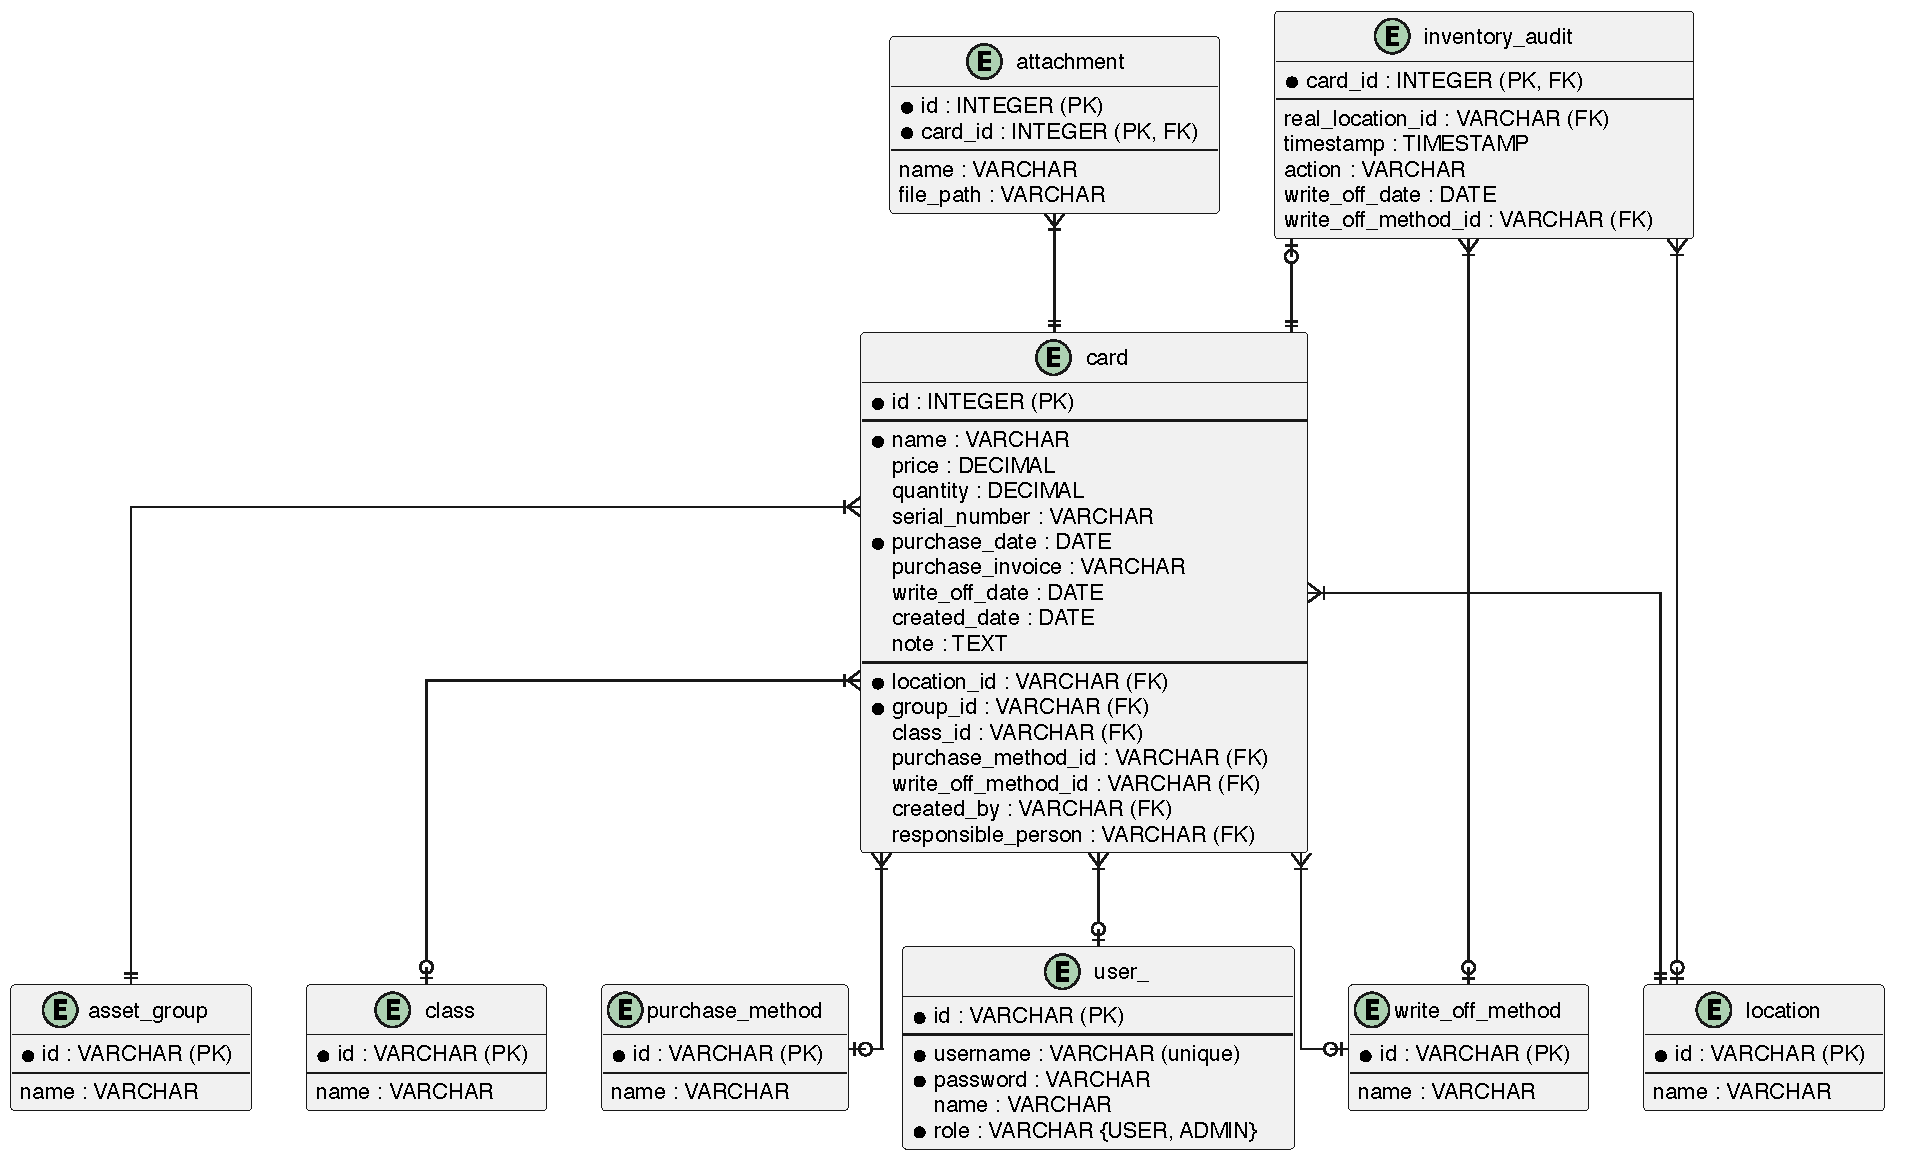
\includegraphics[width=\textwidth]{images/er-diagram.pdf}
	\caption{ER diagram datového modelu}\label{fig:er-diagram}
\end{figure}

\subsection{Popis entit}

\textbf{Card} (majetková karta) je hlavní entita systému. Identifikátor karty je celočíselný, přiřazovaný aplikační logikou. Toto číslo se tiskne na etiketu a~slouží jako inventární číslo v~účetní evidenci. Karta dále obsahuje název, cenu, množství, sériové číslo, datum pořízení, fakturu, poznámku a~vazby na číselníkové entity (umístění, třída, skupina, způsob pořízení, způsob vyřazení) a~uživatele (kdo kartu vytvořil, zodpovědná osoba).

\textbf{Číselníkové entity} (Location, AssetGroup, ClassEntity, PurchaseMethod, WriteOffMethod) sdílejí shodnou strukturu -- textový identifikátor (primární klíč) a~název. Použití přirozeného klíče (natural key) místo umělého auto-increment identifikátoru je záměrné a~inspirováno přístupem ERP systémů -- kódy zadává uživatel ručně (např.\ číslo místnosti, zkratka skupiny) a~v~celém systému se s~nimi pracuje přímo, bez nutnosti překladu přes umělé ID. Číselníkové entity definují přípustné hodnoty pro atributy majetkových karet.

\textbf{Attachment} (příloha) umožňuje připojit soubory ke~kartě majetku. Využívá kompozitní primární klíč složený z~identifikátoru přílohy a~identifikátoru karty.

\textbf{InventoryAudit} (inventurní záznam) uchovává výsledek inventury pro jednu kartu -- skutečné umístění, časové razítko naskenování a~po vyhodnocení i~zvolenou akci (ponechat umístění, změnit umístění, vyřadit). Primární klíč je sdílen s~kartou (\texttt{@MapsId}) -- každá karta může mít nejvýše jeden inventurní záznam.

\textbf{User} (uživatel) obsahuje přihlašovací údaje a~roli (\texttt{USER} nebo \texttt{ADMIN}). Tabulka je v~databázi pojmenována \texttt{user\_} s~podtržítkem, protože \texttt{user} je rezervované slovo v~PostgreSQL. Uživatel je volitelně referencován z~karty jako tvůrce záznamu nebo zodpovědná osoba.



\chapter{Implementace}\label{chap:implementation}

\begin{chapterabstract}
	Kapitola popisuje klíčové implementační detaily jednotlivých částí systému. Zaměřuje se na netriviální části implementace, jejichž řešení vyžadovalo specifický přístup -- například dynamické filtrování pomocí JPA Specification, generování ZPL etiket, bezpečné ukládání přihlašovacích údajů na mobilním zařízení nebo zpracování vstupu z~hardwarového skeneru.
\end{chapterabstract}

\section{Backend}

Backend je implementován jako Spring Boot aplikace s~Maven build systémem a~Javou~21. Zdrojový kód je organizován do doménových balíčků:

\dirtree{%
.1 cz.majetek.
.2 auth\DTcomment{autentizace, JWT, Spring Security}.
.2 card\DTcomment{CRUD karet, filtrování, exporty}.
.2 dictionary\DTcomment{číselníky (lokace, skupiny, třídy, \ldots)}.
.2 inventoryaudit\DTcomment{inventurní audit}.
.2 entity\DTcomment{JPA entity sdílené napříč moduly}.
.2 exception\DTcomment{globální zpracování chyb}.
.2 config\DTcomment{konfigurace (OpenAPI, beans)}.
}

\medskip
Struktura každého modulu odpovídá třívrstvému vzoru z~kapitoly~\ref{sec:backend-arch}, tedy vrstvy controller, service (rozhraní + implementace), repository a~mapper.

\subsection{Filtrování karet majetku}

Filtrování karet (požadavky F-04 a~F-05, viz tabulka~\ref{tab:freq-cards}) je realizováno prostřednictvím JPA Specification API. Třída \texttt{CardSpecification} dynamicky sestavuje predikáty na základě parametrů dotazu -- rozsahy ID, cen, dat, shoda cizích klíčů a~fulltextové vyhledávání.

\begin{listing}[H]
\caption{Fulltextové vyhledávání s~podporou české diakritiky}\label{lst:fulltext}
\begin{minted}[fontsize=\small]{java}
private static void handleFulltext(
    List<Predicate> predicates, String search,
    Root<Card> root, CriteriaBuilder cb) {
  String normalized = search.toLowerCase()
      .replace("\\", "\\\\")
      .replace("%", "\\%")
      .replace("_", "\\_");

  Expression<String> term = cb.function(
      "unaccent", String.class,
      cb.literal(normalized));
  Expression<String> paddedId = cb.function(
      "lpad", String.class,
      root.get("id").as(String.class),
      cb.literal(4), cb.literal("0"));
  Expression<String> name = cb.function(
      "unaccent", String.class,
      cb.lower(root.get("name")));

  predicates.add(cb.or(
      cb.like(name,
          cb.concat("%", cb.concat(term, "%")),
          '\\'),
      cb.like(paddedId,
          cb.concat("%", cb.concat(term, "%")),
          '\\')
  ));
}
\end{minted}
\end{listing}

Vyhledávání využívá PostgreSQL funkci \texttt{unaccent()} pro normalizaci české diakritiky -- dotaz \uv{skrin} nalezne záznam \uv{Skříň}. Identifikátory karet jsou doplněny nulami zleva funkcí \texttt{lpad()}, aby bylo možné vyhledávat i~podle části čísla karty.

Pro generování reportů k~určitému datu slouží metoda \texttt{handleAsOf()}, která vrací pouze karty zakoupené před zadaným datem a~dosud nevyřazené:

\begin{listing}[H]
\caption{Filtr pro point-in-time reporty}\label{lst:asof}
\begin{minted}[fontsize=\small]{java}
private static void handleAsOf(List<Predicate> predicates,
    LocalDate asOf, Root<Card> root, CriteriaBuilder cb) {
  if (asOf == null) return;
  predicates.add(cb.lessThanOrEqualTo(
      root.get("purchaseDate"),
      asOf));
  predicates.add(cb.or(
      root.get("writeOffDate").isNull(),
      cb.greaterThan(root.get("writeOffDate"),
      asOf)));
}
\end{minted}
\end{listing}

\subsection{Generování exportů}

Systém generuje tři typy exportů: PDF reporty (požadavky F-13 až F-15, viz tabulka~\ref{tab:freq-reports}), Excel soubory (F-16) a~ZPL etikety (požadavky F-10 až F-12, viz tabulka~\ref{tab:freq-labels}).

\subsubsection{PDF reporty}

PDF dokumenty jsou generovány knihovnou iText~8 ve třídě \texttt{PdfGenerator}. Reporty jsou vytvářeny v~paměti prostřednictvím \texttt{ByteArrayOutputStream} a~vráceny jako pole bajtů. Pro správné zobrazení českých znaků je použit font Calibri a~čísla jsou formátována s~českou lokalizací.

Systém nabízí tři typy reportů:
\begin{itemize}
	\item Sestavu majetku pro vybranou skupinu.
	\item Souhrnnou sestavu za všechny skupiny.
	\item Sestavu pro vybranou místnost.
\end{itemize}

Ukázka vygenerované sestavy majetkové karty je na obrázku~\ref{fig:pdf-report}.

\begin{figure}[H]
	\centering
	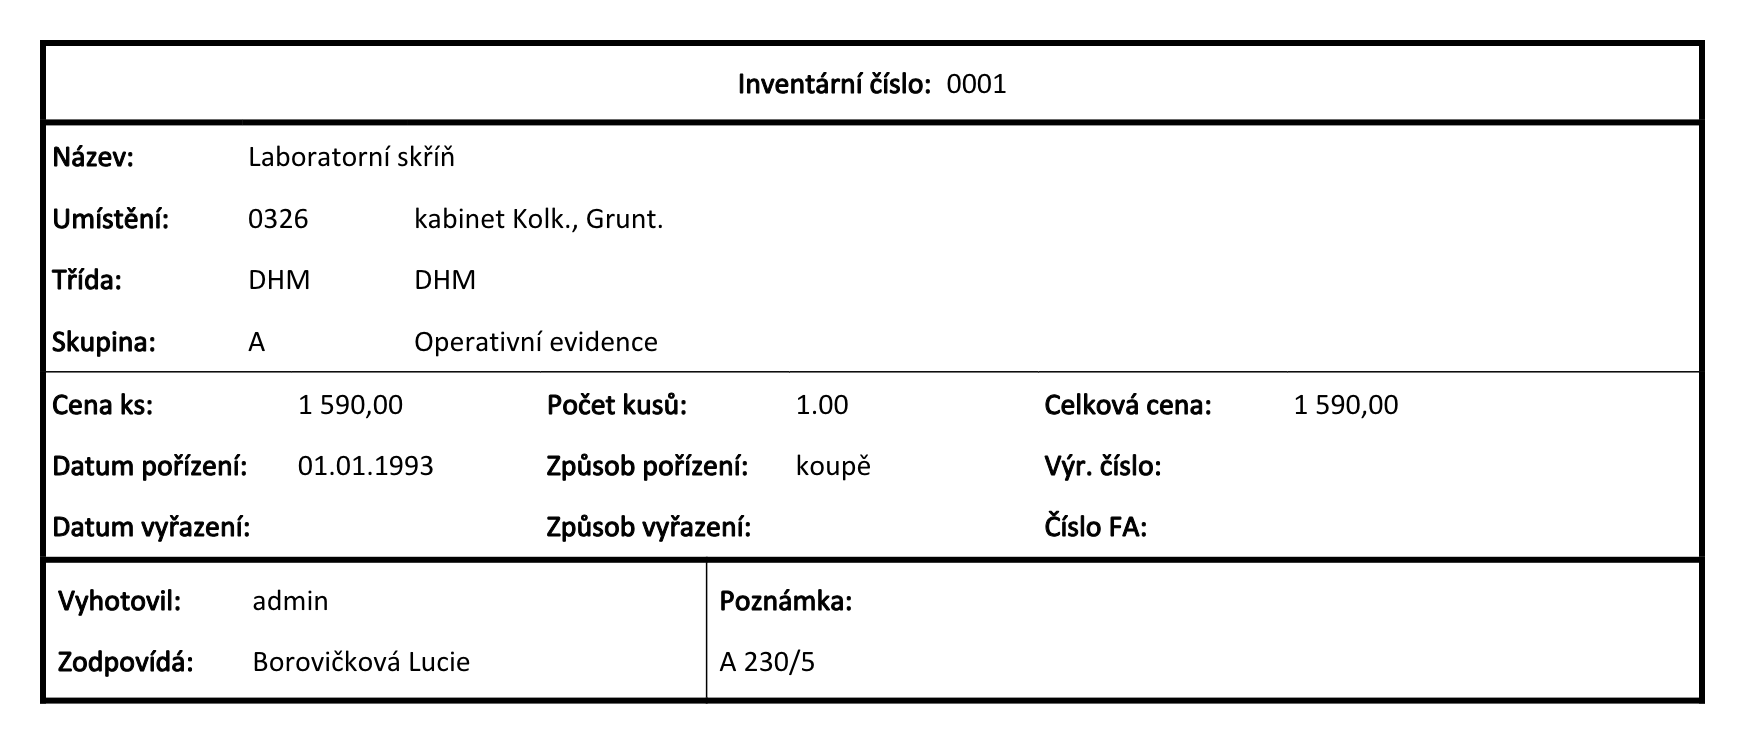
\includegraphics[width=\textwidth]{images/card_pdf_report.png}
	\caption{Ukázka vygenerovaného PDF reportu majetkové karty}
	\label{fig:pdf-report}
\end{figure}

\subsubsection{Excel export}

Export do formátu XLSX využívá knihovnu EasyExcel. Filtrované karty jsou namapovány na \texttt{CardExportDto} se~14~sloupci (ID, název, cena, sériové číslo, umístění, skupina, faktura, data nákupu a~vyřazení, metody, zodpovědná osoba, poznámka) a~zapsány do listu \uv{Karty}.

\subsubsection{ZPL etikety}

Generování etiket využívá šablonový přístup -- ZPL šablona obsahuje zástupné řetězce, které jsou nahrazeny konkrétními daty karty:

\begin{listing}[H]
\caption{Ukázka ZPL šablony etikety (zkráceno)}\label{lst:zpl}
\begin{minted}[fontsize=\small,escapeinside=||]{text}
^XA
^FT530,123^BXN,5,200,0,0,1,_,1
^FH\^FD|\textbf{\color[rgb]{0.6,0,0}\{\{ID\}\}}|^FS
^FT352,234^A0N,58,58^FH\^CI28^FD|\textbf{\color[rgb]{0.6,0,0}\{\{ID\}\}}|^FS^CI27
^FT103,76^A@N,29,29,TT0003M_^FH\^CI28
^FD|\textbf{\color[rgb]{0.6,0,0}\{\{FIRST\_ROW\}\}}|^FS^CI27
^FT103,120^A@N,29,29,TT0003M_^FH\^CI28
^FD|\textbf{\color[rgb]{0.6,0,0}\{\{SECOND\_ROW\}\}}|^FS^CI27
^PQ1,0,1,Y
^XZ
\end{minted}
\end{listing}

Etiketa obsahuje dva Data Matrix kódy (různé velikosti), numerický identifikátor karty, název majetku na dvou řádcích a~logo organizace. Příkaz \texttt{\^{}BXN} generuje Data Matrix kód, \texttt{\^{}FD} definuje obsah pole.

Klíčovým problémem je zalamování názvu majetku na dvouřádkovou etiketu. Třída \texttt{LabelPrinter} pro tento účel načte font skeneru Zebra a~pomocí Java třídy \texttt{TextLayout} vypočítá skutečnou šířku textu v~milimetrech:

\begin{listing}[H]
\caption{Výpočet šířky textu pro ZPL etiketu}\label{lst:willfit}
\begin{minted}[fontsize=\small]{java}
private boolean willFit(String text) {
  float width = new TextLayout(
      text, ZEBRA_FONT, FONT_RENDER_CONTEXT)
      .getAdvance();
  return MAX_PRINT_WIDTH_MM > (width / PRINTER_DPI) * MM_PER_INCH;
}
\end{minted}
\end{listing}

Metoda převádí šířku z~bodů na milimetry a~porovnává ji s~konstantou \texttt{MAX\_PRINT\_WIDTH\_MM} (maximální šířka tisknutelné oblasti etikety). Text je poté rozdělen po slovech na dva řádky tak, aby se každý vešel na etiketu. Ukázka vytištěných etiket je na obrázku~\ref{fig:labels}.

\begin{figure}[H]
	\centering
	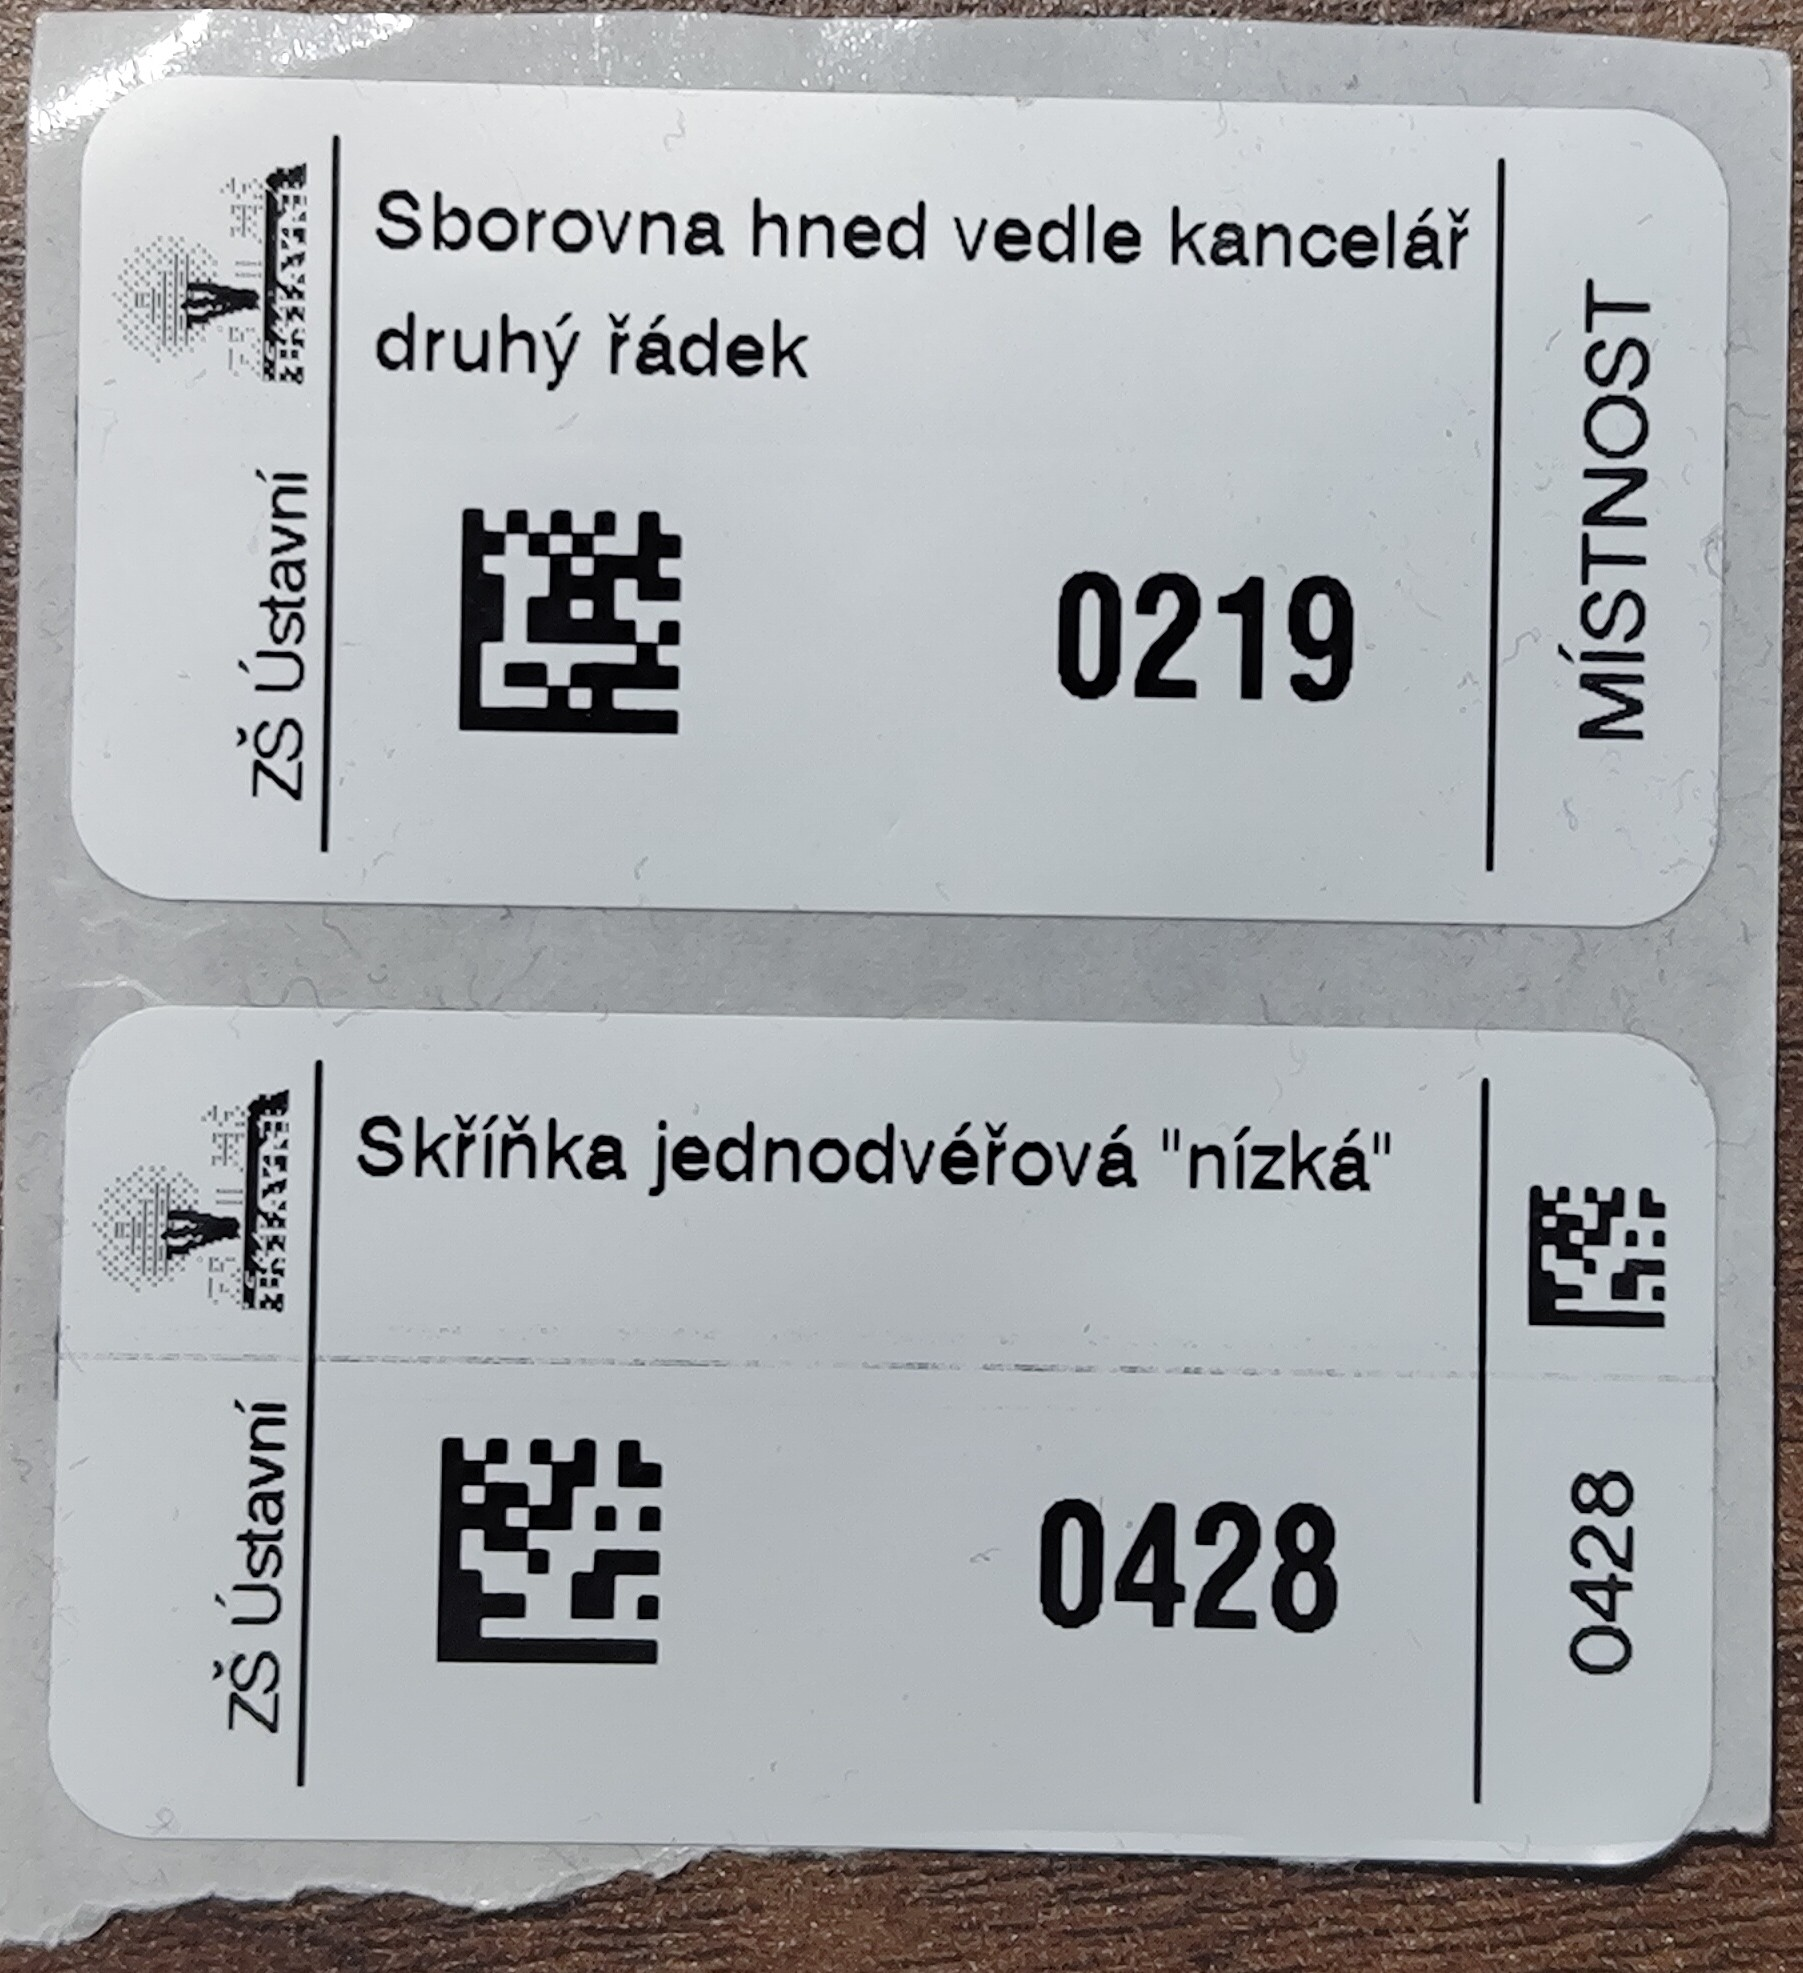
\includegraphics[width=0.5\textwidth]{images/labels.jpg}
	\caption{Vytištěné etikety -- štítek lokace (nahoře) a~štítek majetku (dole)}
	\label{fig:labels}
\end{figure}

Hotové etikety jsou odeslány na tiskárnu Zebra prostřednictvím Zebra Cloud API (\texttt{POST} na \texttt{api.zebra.com}). Vzhledem k~tomu, že bezplatný tarif API umožňuje pouze 100~požadavků denně, je alternativně nabídnuto stažení ZPL souboru pro lokální tisk.

\subsection{Inventurní audit}
Inventurní audit (požadavky F-17 až F-25, viz tabulky~\ref{tab:freq-inventory-mobile} a~\ref{tab:freq-inventory-web}) je na straně backendu implementován ve~dvou fázích:
\begin{enumerate}
	\item Import dat z~mobilní aplikace.
	\item Vyhodnocení s~projekcí změn.
\end{enumerate}

Celý inventurní proces od založení inventury přes skenování až po promítnutí změn je znázorněn na obrázku~\ref{fig:activity-inventory}.

\begin{figure}[H]
	\centering
	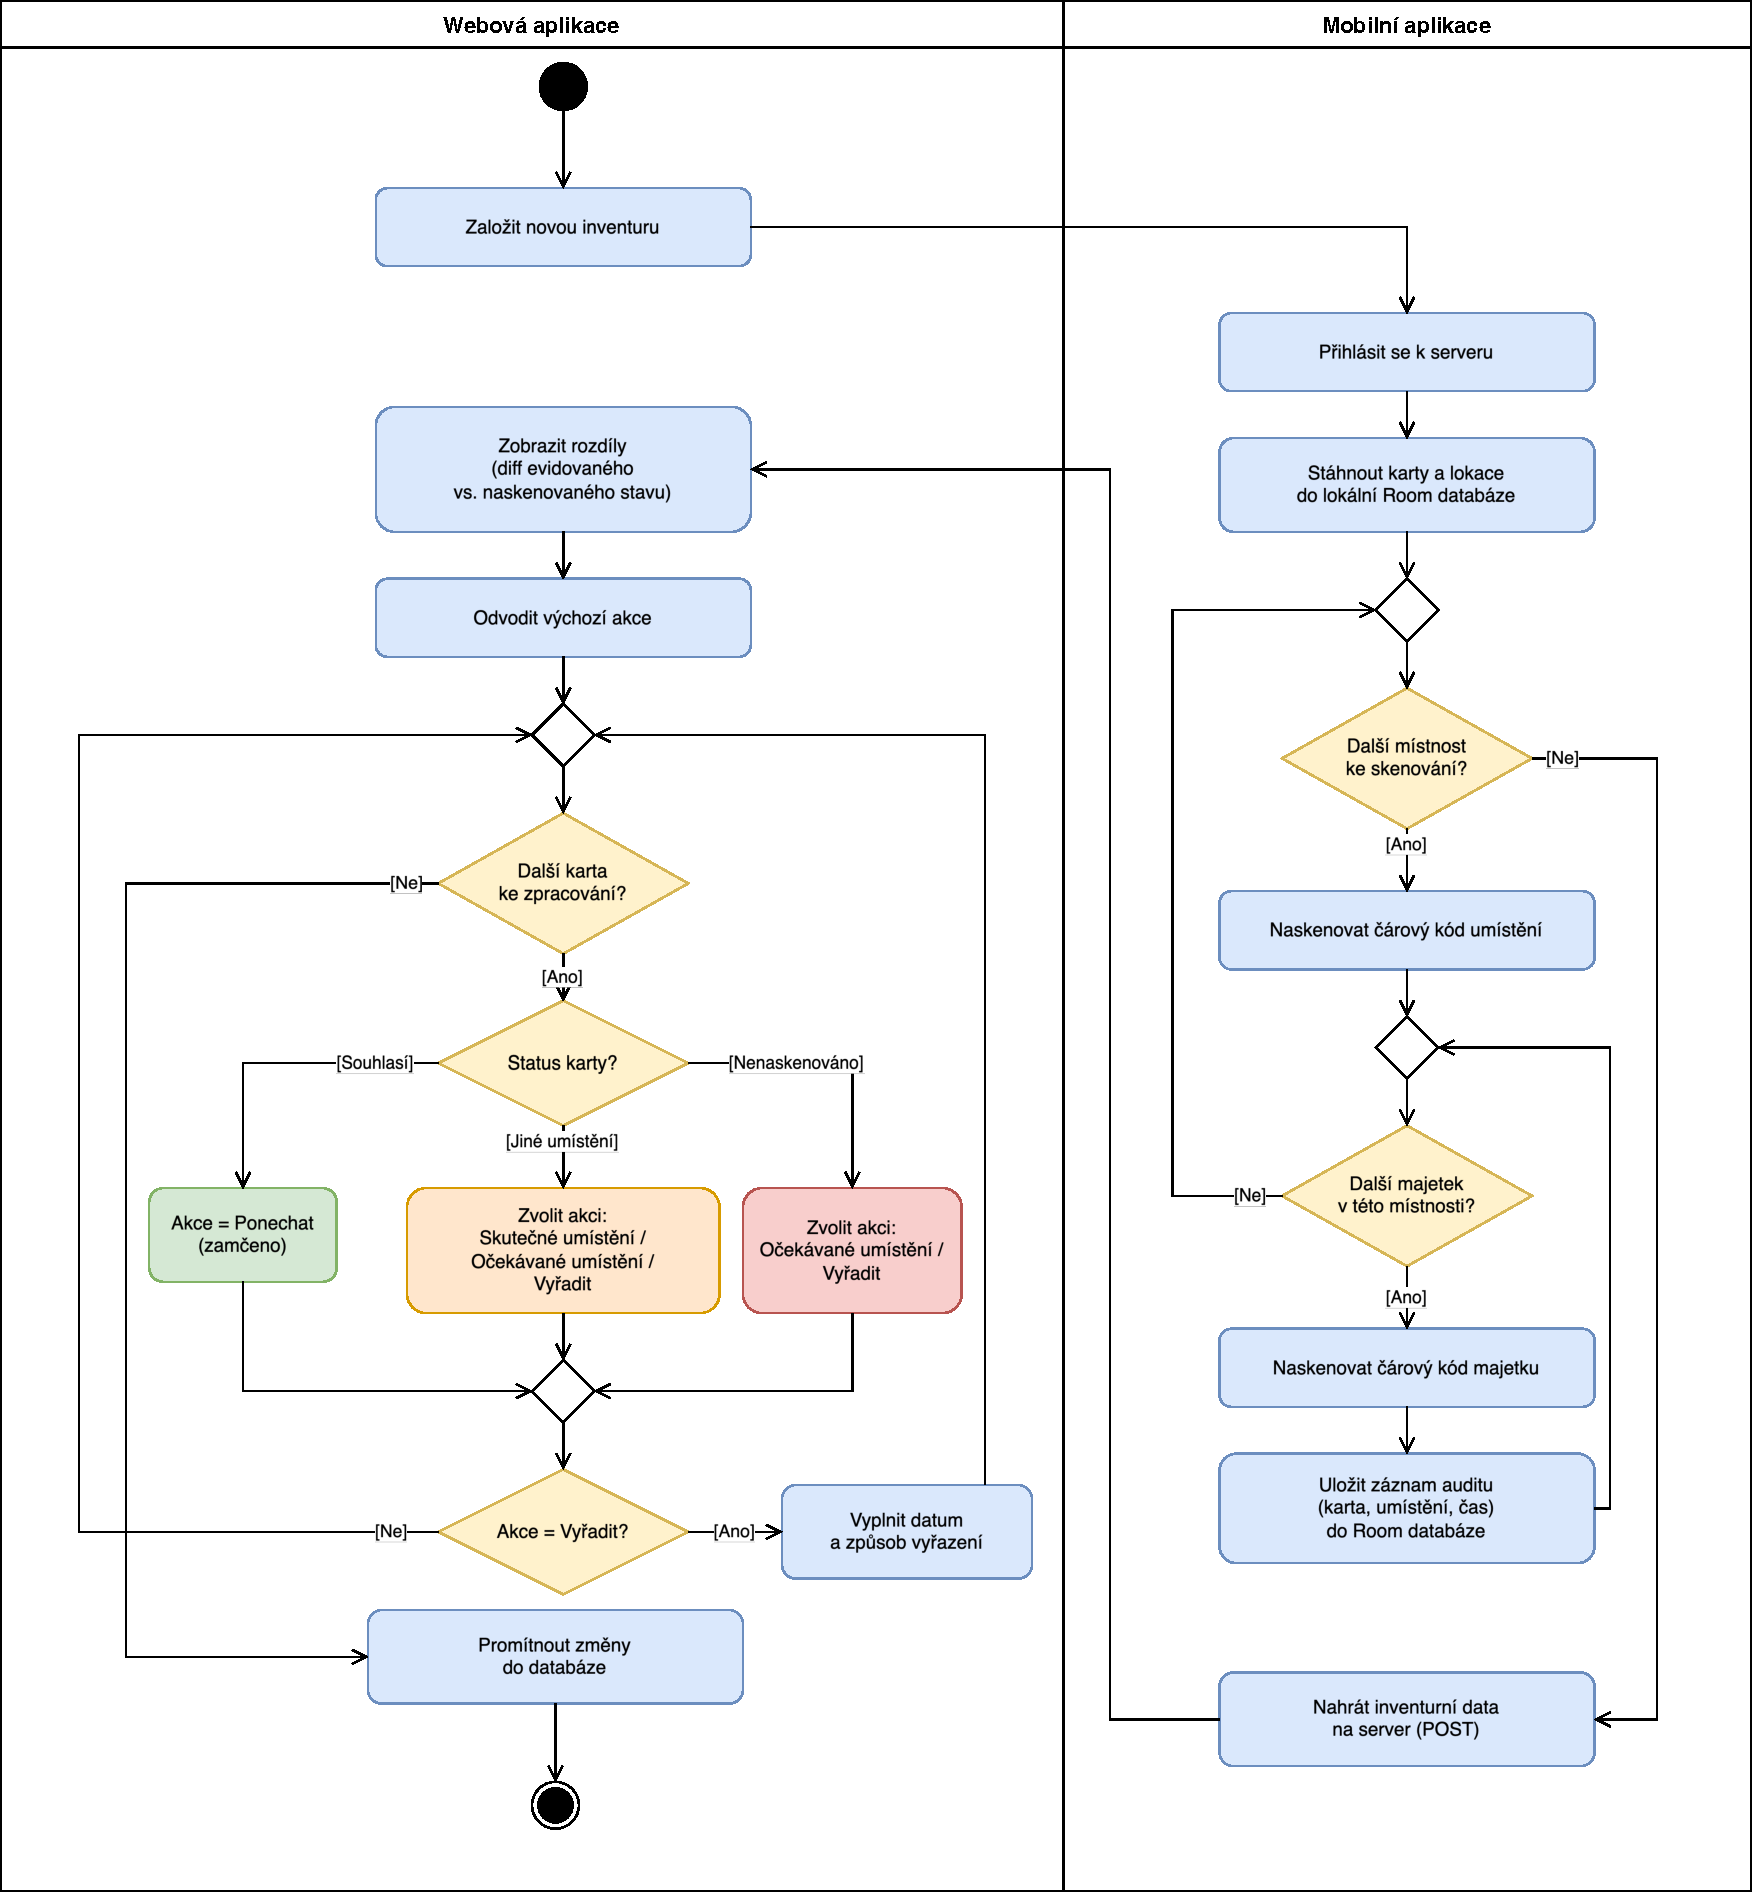
\includegraphics[width=0.75\textwidth]{images/activity-inventory.pdf}
	\caption{Diagram aktivit -- inventurní proces}
	\label{fig:activity-inventory}
\end{figure}

\subsubsection{Import dat}

Endpoint \texttt{POST /api/inventory-audit/insert-many} přijímá hromadný zápis inventurních záznamů z~mobilní aplikace. Každý záznam obsahuje identifikátor karty, identifikátor reálného umístění a~časové razítko naskenování. Záznamy jsou vloženy do tabulky \texttt{inventory\_audit} s~vazbou na existující kartu.

\subsubsection{Výpočet rozdílů}

Klíčovou částí inventurního procesu je porovnání skutečného stavu (naskenovaného umístění) s~evidovaným stavem (umístění v~databázi). Toto porovnání provádí MapStruct mapper:

\begin{listing}[H]
\caption{Výpočet inventurního statusu v~mapperu}\label{lst:mapstatus}
\begin{minted}[fontsize=\small]{java}
default InventoryAuditStatus mapStatus(Card entity) {
  if (entity.getInventoryAudit() == null
      || entity.getInventoryAudit()
           .getRealLocation() == null) {
    return InventoryAuditStatus.WRONG;
  }
  String realId = entity.getInventoryAudit()
      .getRealLocation().getId();
  String expectedId = entity.getLocation().getId();
  if (!realId.equals(expectedId)) {
    return InventoryAuditStatus.WARN;
  }
  return InventoryAuditStatus.CORRECT;
}
\end{minted}
\end{listing}

Mapper vrací tři stavy: \texttt{CORRECT} (lokace souhlasí), \texttt{WARN} (lokace se liší) a~\texttt{WRONG} (karta nebyla naskenována). U~stavu \texttt{CORRECT} je automaticky zvolena akce \texttt{KEEP} (ponechat) a~uživatel ji nemůže změnit. U~stavu \texttt{WARN} může uživatel zvolit akci \texttt{RL} (real location -- přesunout na skutečnou lokaci), \texttt{EL} (expected location -- ponechat na původní lokaci) nebo \texttt{WRITE\_OFF} (vyřadit). U~stavu \texttt{WRONG} jsou dostupné akce \texttt{EL} a~\texttt{WRITE\_OFF}.

\subsubsection{Projekce změn}

Endpoint \texttt{POST /api/inventory-audit/project} aplikuje rozhodnutí uživatele na databázi. Pro akci \texttt{RL} je aktualizováno umístění karty, pro \texttt{WRITE\_OFF} jsou nastaveny datum a~způsob vyřazení. Po dokončení projekce jsou inventurní záznamy smazány.

\subsection{Cachování číselníků}

Číselníkové entity (lokace, skupiny, třídy, způsoby pořízení a~vyřazení) se mění zřídka, ale jsou načítány při každém zobrazení formuláře nebo tabulky. Pro snížení zátěže databáze je implementováno cachování prostřednictvím Spring Cache a~knihovny Caffeine:

\begin{listing}[H]
\caption{Cachování číselníkových dat}\label{lst:cache}
\begin{minted}[fontsize=\small]{java}
@Cacheable("locations")
public List<Location> getAll() {
  return locationRepository.findAll();
}

@CacheEvict(value = "locations", allEntries = true)
public Location create(Location location) {
  // ...
  return locationRepository.save(location);
}
\end{minted}
\end{listing}

Cache je nakonfigurována s~maximální kapacitou 500 záznamů a~expirací 10 minut po zápisu. Při jakékoliv modifikaci číselníku (vytvoření, přejmenování, smazání) jsou všechny záznamy příslušné cache invalidovány anotací \texttt{@CacheEvict}.

\subsection{Mapování DTO}

Knihovna MapStruct generuje mapovací kód v~době kompilace na základě anotací na rozhraní mapperu. Následující ukázka demonstruje mapování entity \texttt{Card} na \texttt{CardDto}, kde jsou vnořené relace převedeny na ploché atributy:

\begin{listing}[H]
\caption{MapStruct mapper pro kartu majetku (zkráceno)}\label{lst:mapper}
\begin{minted}[fontsize=\small]{java}
@Mapper(componentModel = "spring")
public interface ICardMapper {
  @Mapping(source = "location.id", target = "locationId")
  @Mapping(source = "location.name", target = "locationName")
  @Mapping(source = "group.id", target = "groupId")
  @Mapping(source = "group.name", target = "groupName")
  // ...
  CardDto toDto(Card card);

  @Mapping(source = "locationId", target = "location",
           qualifiedByName = "toLocation")
  Card toEntity(CardChangeDto dto);

  @Named("toLocation")
  default Location toLocation(String id) {
    if (id == null) return null;
    Location l = new Location();
    l.setId(id);
    return l;
  }
}
\end{minted}
\end{listing}

Metoda \texttt{toDto()} převádí vnořené entity na ploché identifikátory a~názvy pro API odpověď. Opačný směr (\texttt{toEntity()}) využívá anotaci \texttt{@Named} pro vlastní metody, které rekonstruují entitu pouze s~nastaveným identifikátorem~-- JPA poté zajistí vazbu na existující záznam v~databázi.

\section{Frontend}

\subsection{Struktura projektu}

Frontend je vytvořen nástrojem Vite s~Reactem~19 a~TypeScriptem. Zdrojový kód je organizován následovně:

\needspace{12\baselineskip}
\dirtree{%
.1 src/.
.2 components\DTcomment{UI komponenty podle domény}.
.3 card\DTcomment{správa karet majetku}.
.3 dictionary\DTcomment{generické číselníkové komponenty}.
.3 inventoryAudit\DTcomment{vyhodnocení inventury}.
.3 report\DTcomment{modální okna pro reporty}.
.2 hooks/queries\DTcomment{TanStack Query hooky}.
.2 pages\DTcomment{komponenty na úrovni route}.
.2 services\DTcomment{Axios API volání}.
.2 schemas\DTcomment{Zod validační schémata}.
.2 store\DTcomment{Zustand auth store}.
.2 types\DTcomment{TypeScript typy}.
}

\subsection{Správa karet majetku}

Stránka pro správu karet (požadavky F-01 až F-07, viz obrázek~\ref{fig:card-page}) využívá rozložení master-detail. Levý panel (\texttt{CardListPanel}) zobrazuje seznam karet s~fulltextovým vyhledáváním, tříděním a~pokročilým filtrováním. Pravý panel zobrazuje detail vybrané karty nebo formulář pro vytvoření nové:

\begin{figure}[H]
	\centering
	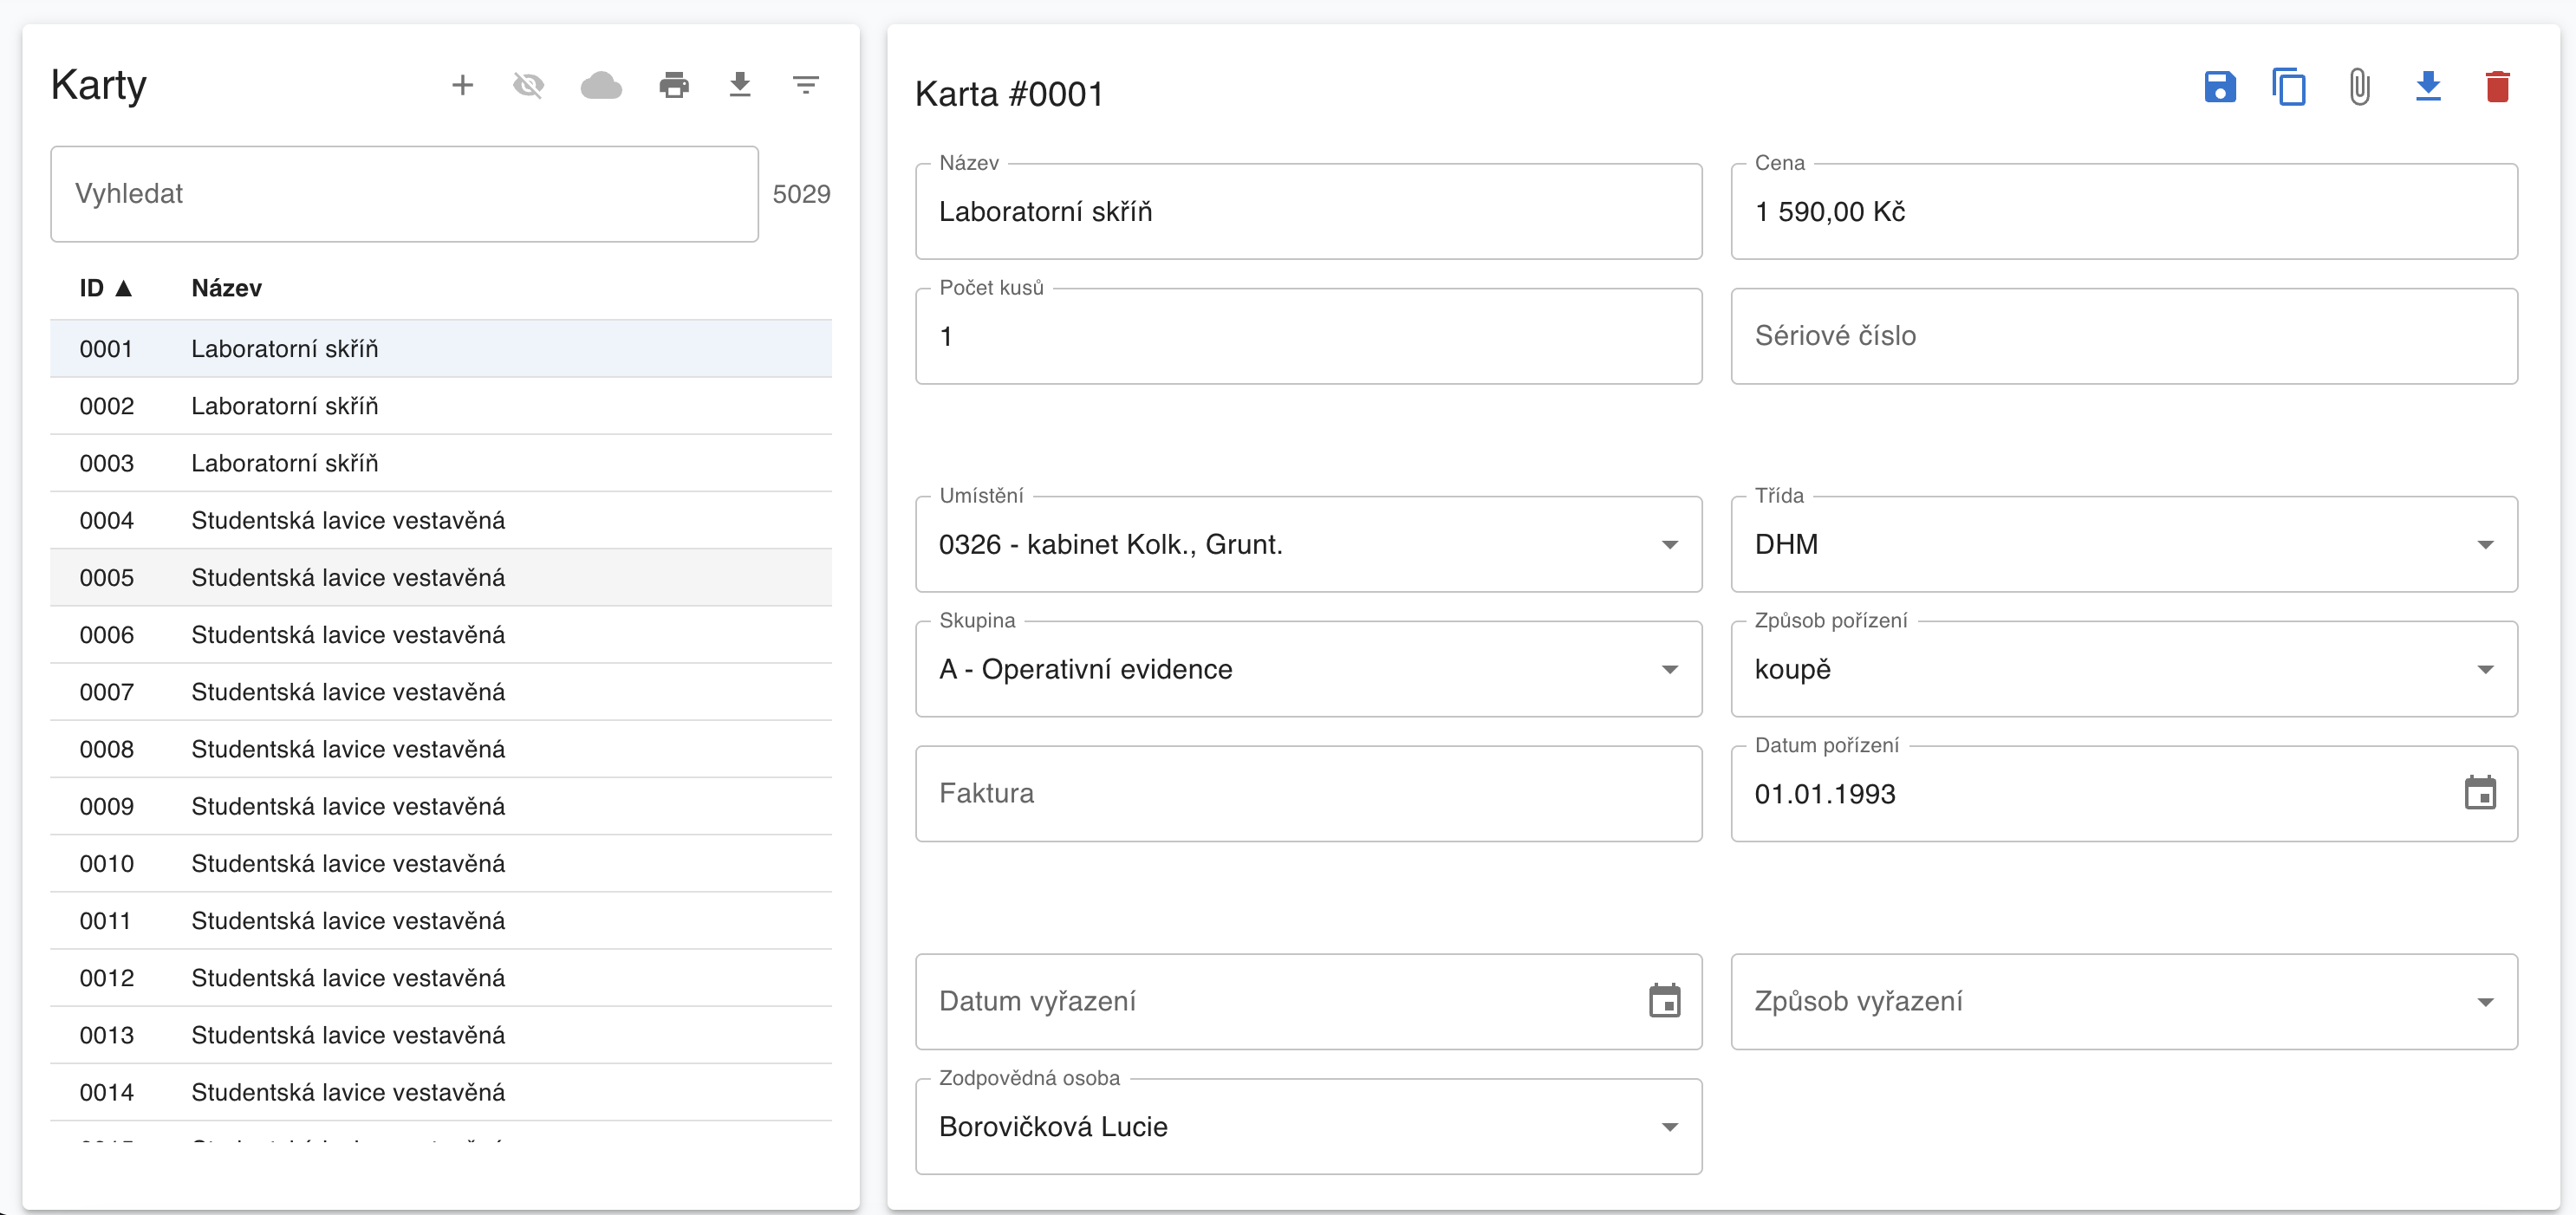
\includegraphics[width=\textwidth]{images/card_page.png}
	\caption{Stránka karet majetku -- master-detail layout}
	\label{fig:card-page}
\end{figure}

\begin{listing}[H]
\caption{Master-detail layout stránky karet (zkráceno)}\label{lst:cardpage}
\begin{minted}[fontsize=\small,escapeinside=@@]{tsx}
type CardSelection =
  | { type: "existing"; id: string }
  | { type: "new" };

const CardPage = () => {
  const [selection, setSelection] =
    useState<CardSelection>();
  const selectedId = selection?.type === "existing"
    ? selection.id : undefined;
  return (
    <div className="p-6 flex">
      <CardListPanel
        selectedCardId={selectedId}
        onSelectCard={(id) => setSelection(
          id ? { type: "existing", id } : @\textcolor[HTML]{8F2200}{\textbf{undefined}}@)}
        onNewCard={() =>
          setSelection({ type: "new" })}
      />
      <Paper className="w-2/3 p-4" elevation={3}>
        {selection?.type === "new" ? (
          <CardCreateView ... />
        ) : selection?.type === "existing" ? (
          <CardDetailView
            cardId={selection.id} ... />
        ) : (
          <Typography>Vyberte kartu vlevo</Typography>
        )}
      </Paper>
    </div>
  );
};
\end{minted}
\end{listing}

Client-side vyhledávání využívá knihovnu Fuse.js pro fuzzy matching a~React hook \texttt{useDeferredValue} pro odložení vykreslení při rychlém psaní, čímž je zajištěna plynulost uživatelského rozhraní.

\subsection{Generický vzor pro číselníky}

Pět číselníkových stránek (lokace, skupiny, třídy, způsoby pořízení a~vyřazení) sdílí jedinou generickou komponentu \texttt{DictionaryPage<T>}. Komponenta přijímá query a~mutační hooky jako vlastnosti a~vykresluje tabulku s~operacemi vytvoření, přejmenování a~smazání:

\begin{listing}[H]
\caption{Typové rozhraní generické číselníkové komponenty}\label{lst:dictprops}
\begin{minted}[fontsize=\small]{tsx}
interface DictionaryPageProps<T extends DictionaryEntity> {
  readonly title: string;
  readonly useItems: () => UseQueryResult<T[]>;
  readonly useCreate: () => UseMutationResult<T, ...>;
  readonly useUpdate: () => UseMutationResult<...>;
  readonly useDelete: () => UseMutationResult<...>;
  readonly extraRowActions?: (item: T) => ReactNode;
}
\end{minted}
\end{listing}

Konkrétní stránky jsou pouze tenké wrappery, které předávají příslušné hooky:

\begin{listing}[H]
\caption{Stránka lokací jako wrapper nad generickou komponentou}\label{lst:locationpage}
\begin{minted}[fontsize=\small]{tsx}
const LocationPage = () => (
  <DictionaryPage<Location>
    title="Umístění"
    useItems={useLocations}
    useCreate={useCreateLocation}
    useUpdate={useUpdateLocation}
    useDelete={useDeleteLocation}
    extraRowActions={(loc) => (
      <IconButton onClick={
        () => printMutation.mutate(loc.id)}>
        <PrintIcon />
      </IconButton>
    )}
  />
);
\end{minted}
\end{listing}

Stránka lokací navíc přidává tlačítko tisku etikety prostřednictvím vlastnosti \texttt{extraRowActions}. Editace názvu probíhá přímo v~tabulce -- komponenta \texttt{DictionaryRow} ukládá změny při opuštění textového pole (událost \texttt{onBlur}). Ukázka výsledné stránky pro správu lokací je na obrázku~\ref{fig:location-page}.

\begin{figure}[H]
	\centering
	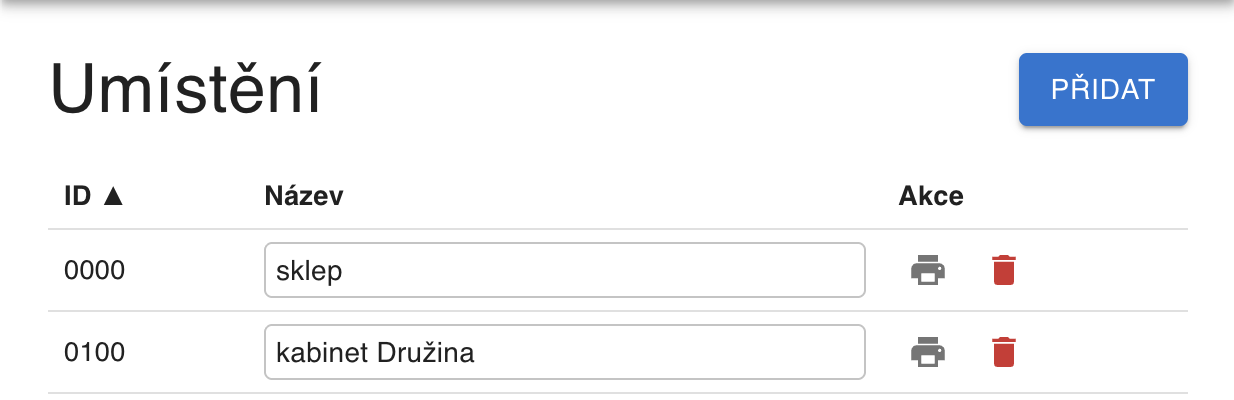
\includegraphics[width=0.7\textwidth]{images/location_page.png}
	\caption{Číselníková stránka Umístění -- instance generické komponenty \texttt{DictionaryPage}}
	\label{fig:location-page}
\end{figure}

\subsection{Formuláře a~validace}

Formuláře v~aplikaci využívají knihovnu React Hook Form v~kombinaci s~validační knihovnou Zod. Validační schéma slouží zároveň jako dokumentace očekávaného formátu dat:

\begin{listing}[H]
\caption{Zod validační schéma pro číselníkový záznam}\label{lst:zodschema}
\begin{minted}[fontsize=\small]{typescript}
export function createDictionarySchema(maxIdLength = 20) {
  return z.object({
    id: z.string()
      .min(1, "ID je povinné.")
      .max(maxIdLength,
        `ID nesmí být delší než ${maxIdLength} znaků.`),
    name: z.string()
      .max(255, "Název nesmí být delší než 255 znaků.")
      .transform((v) => v.trim() === "" ? null : v.trim())
      .nullable(),
  });
}
\end{minted}
\end{listing}

Schéma je propojeno s~formulářem prostřednictvím resolveru \texttt{zodResolver}, který automaticky mapuje validační chyby na příslušná pole formuláře.

\subsection{Vyhodnocení inventury}

Stránka pro vyhodnocení inventury (požadavky F-22 až F-25, viz obrázek~\ref{fig:differences-page}) zobrazuje tabulku (MUI DataGrid) s~barevně odlišenými řádky podle statusu:
\begin{itemize}
	\item zelená -- \texttt{CORRECT} (umístění souhlasí),
	\item oranžová -- \texttt{WARN} (umístění se liší),
	\item červená -- \texttt{WRONG} (karta nebyla naskenována).
\end{itemize}

Stavovou logiku zapouzdřuje custom hook \texttt{useDifferenceEntries}. Ten zajišťuje:
\begin{itemize}
	\item Načtení rozdílů ze serveru prostřednictvím TanStack Query.
	\item Odvození výchozích akcí: \texttt{CORRECT} automaticky \texttt{KEEP} (nelze změnit), \texttt{WARN} automaticky \texttt{RL} (přijmout skutečné umístění), \texttt{WRONG} vyžaduje manuální rozhodnutí.
	\item Optimistické aktualizace -- změna akce se okamžitě projeví v~UI a~zároveň je odeslána na server. Při chybě je stav vrácen zpět.
	\item Validaci před projekcí -- tlačítko \uv{Promítnout} je zablokováno, pokud existuje karta se statusem \texttt{WRONG} bez zvolené akce, nebo karta s~akcí \texttt{WRITE\_OFF} bez vyplněného data či způsobu vyřazení.
\end{itemize}

\begin{figure}[H]
	\centering
	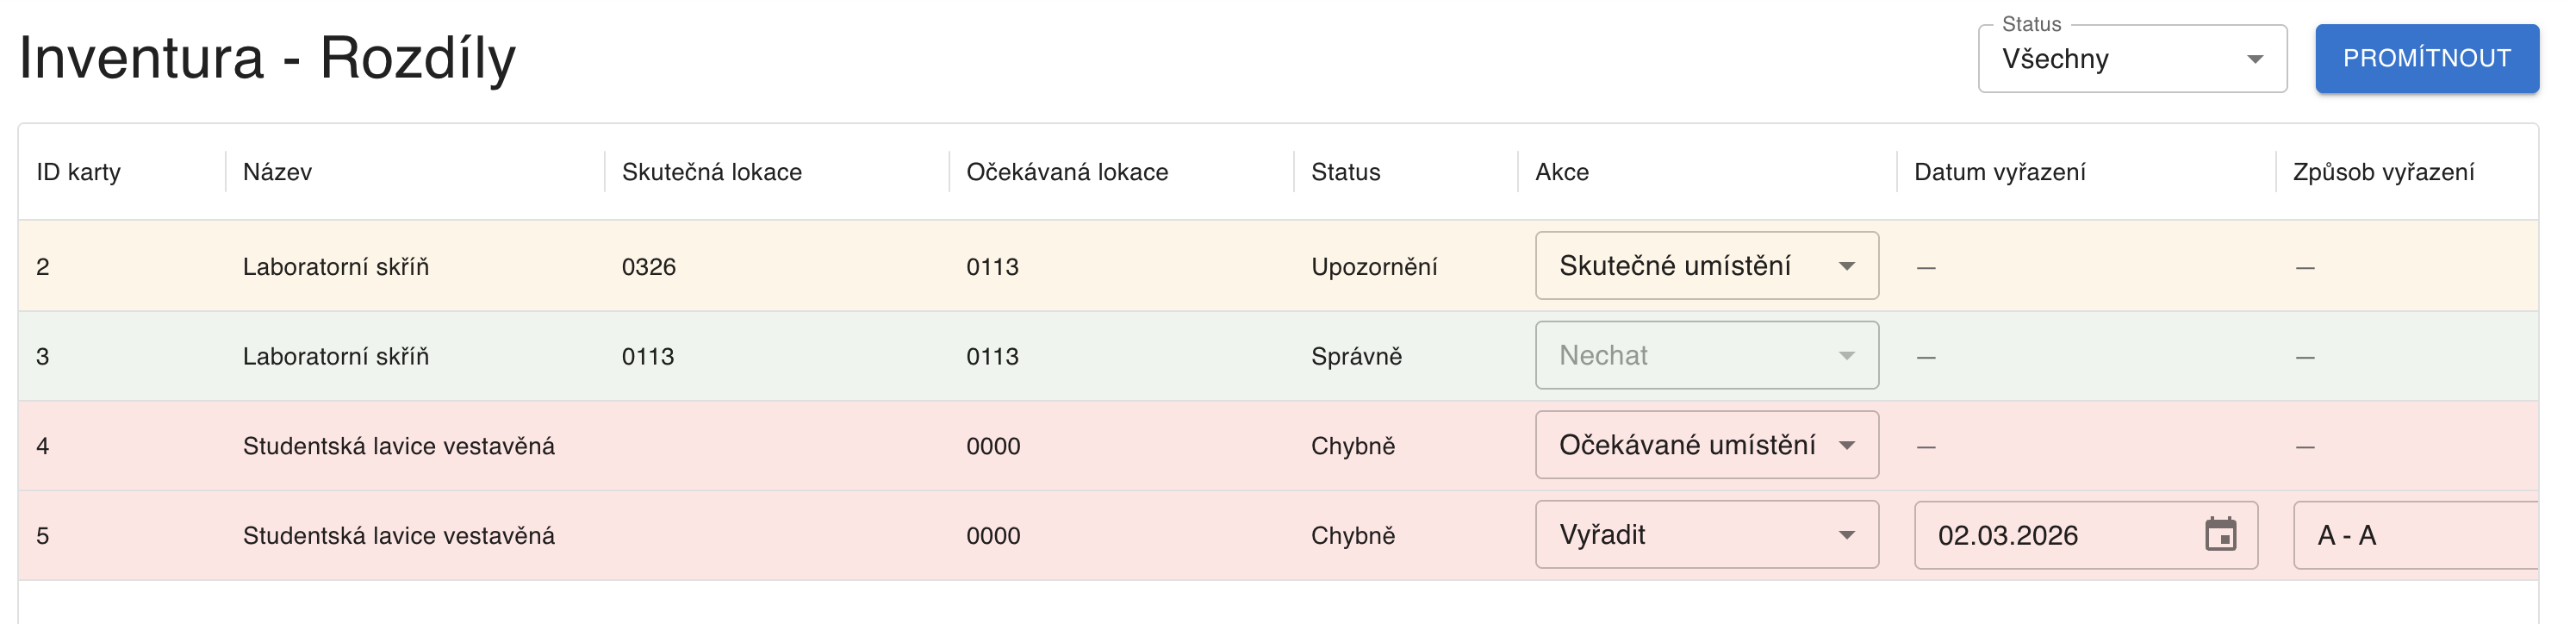
\includegraphics[width=\textwidth]{images/differences_page.png}
	\caption{Stránka vyhodnocení inventury -- barevné řádky podle statusu}
	\label{fig:differences-page}
\end{figure}

\subsection{Autentizace na frontendu}

Autentizační stav (uživatel, JWT token, expirace) je spravován knihovnou Zustand v~jednom globálním store. Klíčovým prvkem je Axios interceptor, který automaticky obnovuje vypršelý token:

\begin{listing}[H]
\caption{Axios interceptor pro automatické obnovení tokenu}\label{lst:interceptor}
\begin{minted}[fontsize=\small]{typescript}
let refreshPromise: Promise<AuthResponse> | null = null;
function refreshOnce() {
  if (!refreshPromise) {
    refreshPromise = refresh()
      .finally(() => { refreshPromise = null; });
  }
  return refreshPromise;
}

authorizedRequest.interceptors.request.use(async (config) => {
  const { token, expiresIn, setAuth, clearAuth }
    = useAuthStore.getState();
  if (token && expiresIn
      && new Date(expiresIn) <= new Date()) {
    try {
      const refreshed = await refreshOnce();
      setAuth(refreshed.user, refreshed.token,
              refreshed.expiresIn);
      config.headers.Authorization =
        `Bearer ${refreshed.token}`;
    } catch {
      clearAuth();
      throw new axios.Cancel("Token refresh failed");
    }
  } else if (token) {
    config.headers.Authorization = `Bearer ${token}`;
  }
  return config;
});
\end{minted}
\end{listing}

Interceptor před každým požadavkem zkontroluje expiraci tokenu. Pokud token vypršel, zavolá endpoint \texttt{/api/auth/refresh} (refresh token je přenášen v~\texttt{httpOnly} cookie) a~po úspěšné obnově pokračuje s~novým tokenem. Jelikož server při každém refresh vygeneruje nový refresh token a~starý invaliduje (rotace), je nutné zajistit, aby se refresh volal nejvýše jednou -- při více souběžných požadavcích sdílejí všechny jeden \texttt{Promise} (mutex pattern). Odpovědi se stavovým kódem 401 jsou zachyceny response interceptorem, který provede stejný proces a~zopakuje původní požadavek.

Všechny chráněné stránky jsou obaleny komponentou \texttt{PrivateRoute}, která ověřuje přítomnost platného tokenu v~Zustand store a~nepřihlášeného uživatele přesměruje na přihlašovací stránku.

\needspace{8\baselineskip}
\section{Mobilní aplikace}

\subsection{Struktura projektu}

Mobilní aplikace je nativní Android projekt v~Javě~21 s~build systémem Gradle (Kotlin DSL). Architektura aplikace (jedna Activity, tři fragmenty, lokální databáze) byla popsána v~kapitole~\ref{sec:mobile-arch}. Tato sekce se zaměřuje na implementační detaily.

\subsection{Integrace se čtečkou Zebra}

Hardwarový skener Zebra TC22 emuluje klávesnici -- naskenovaný kód je odeslán jako sekvence klávesových událostí zakončená klávesou Enter nebo Tab. Pro spolehlivé zachycení vstupu je implementován dual-listener pattern, kde každé vstupní pole registruje dva listenery současně:

\begin{listing}[H]
\caption{Dual-listener pro zachycení vstupu ze skeneru Zebra}\label{lst:duallistener}
\begin{minted}[fontsize=\small]{java}
private void attachScanListeners(
    EditText input, Consumer<String> handler) {
  input.setOnEditorActionListener(
      (tv, actionId, event) -> {
    if (isConfirmAction(event, actionId)) {
      handler.accept(tv.getText().toString().trim());
      return true;
    }
    return false;
  });
  input.setOnKeyListener((v, keyCode, event) -> {
    if (isHardwareEnter(event, keyCode)) {
      handler.accept(input.getText().toString().trim());
      return true;
    }
    return false;
  });
}
\end{minted}
\end{listing}

Metoda \texttt{attachScanListeners()} registruje dva listenery na vstupní pole: \texttt{OnEditorActionListener} zachytává událost \texttt{IME\_ACTION\_DONE} ze softwarové klávesnice, zatímco \texttt{OnKeyListener} reaguje na hardwarové klávesy skeneru (Enter/Tab). Kombinací obou listenerů je zajištěno, že žádný sken nebude ztracen. Metoda je volána pro obě vstupní pole (umístění i~majetek) s~příslušným handlerem.

Naskenované kódy jsou rozlišeny podle formátu: kódy začínající prefixem \uv{L} identifikují umístění (místnost), čistě numerické kódy identifikují majetkovou kartu. Po naskenování karty aplikace vizuálně signalizuje výsledek barvou pozadí: zelená pokud je karta ve správném umístění, oranžová pokud je v~jiném umístění a~červená pokud karta nebyla nalezena v~databázi.

Inventurní postup je vizualizován dvěma kruhovými ukazateli průběhu, které vykresluje vlastní komponenta \texttt{CircularInventoryProgressView} -- levý zobrazuje poměr naskenovaných karet v~aktuálním umístění, pravý celkový postup inventury napříč všemi umístěními. Celá obrazovka skenování je zachycena na obrázku~\ref{fig:scanning-page}.

\begin{figure}[H]
	\centering
	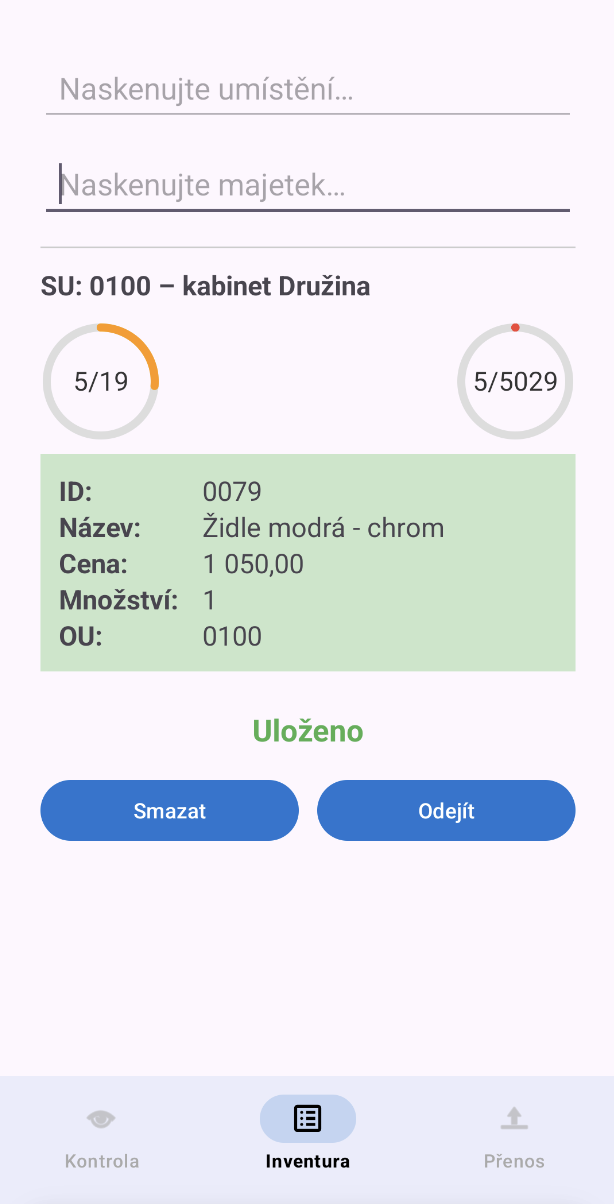
\includegraphics[width=0.35\textwidth]{images/scanning_page.png}
	\caption{Obrazovka skenování inventury s~kruhovým progressem}
	\label{fig:scanning-page}
\end{figure}

\subsection{Room databáze a~offline režim}

Lokální databáze je realizována knihovnou Room se třemi entitami. Klíčová je tabulka \texttt{inventory\_audit}, kde primární klíč \texttt{card\_id} zajišťuje, že každá karta má nejvýše jeden inventurní záznam:

\begin{listing}[H]
\caption{Room entita inventurního záznamu}\label{lst:roomaudit}
\begin{minted}[fontsize=\small]{java}
@Entity(tableName = "inventory_audit",
  foreignKeys = {
    @ForeignKey(entity = CardEntity.class,
      parentColumns = "id", childColumns = "card_id"),
    @ForeignKey(entity = LocationEntity.class,
      parentColumns = "id",
      childColumns = "real_location_id")
  })
public class InventoryAuditEntity {
  @PrimaryKey
  @ColumnInfo(name = "card_id") private int cardId;
  @ColumnInfo(name = "real_location_id")
  private String realLocationId;
  private long timestamp;
}
\end{minted}
\end{listing}

Opakované naskenování téže karty aktualizuje existující záznam díky strategii \texttt{OnConflictStrategy.REPLACE} v~DAO metodě \texttt{upsert()}. Pro zajištění thread safety běží veškeré databázové operace na jednom vyhrazeném vlákně, které je vytvořeno voláním \texttt{Executors.newSingleThreadExecutor()}.

\subsection{Synchronizace se serverem}

Synchronizace dat probíhá na explicitní pokyn uživatele (viz obrázek~\ref{fig:data-transfer-page}). Komunikaci znázorňuje sekvenční diagram~\ref{fig:sequence-sync}. Celý proces orchestruje třída \texttt{DataSyncRepository}; databáze je implementována jako singleton sdílený napříč aplikací:

\begin{figure}[H]
	\centering
	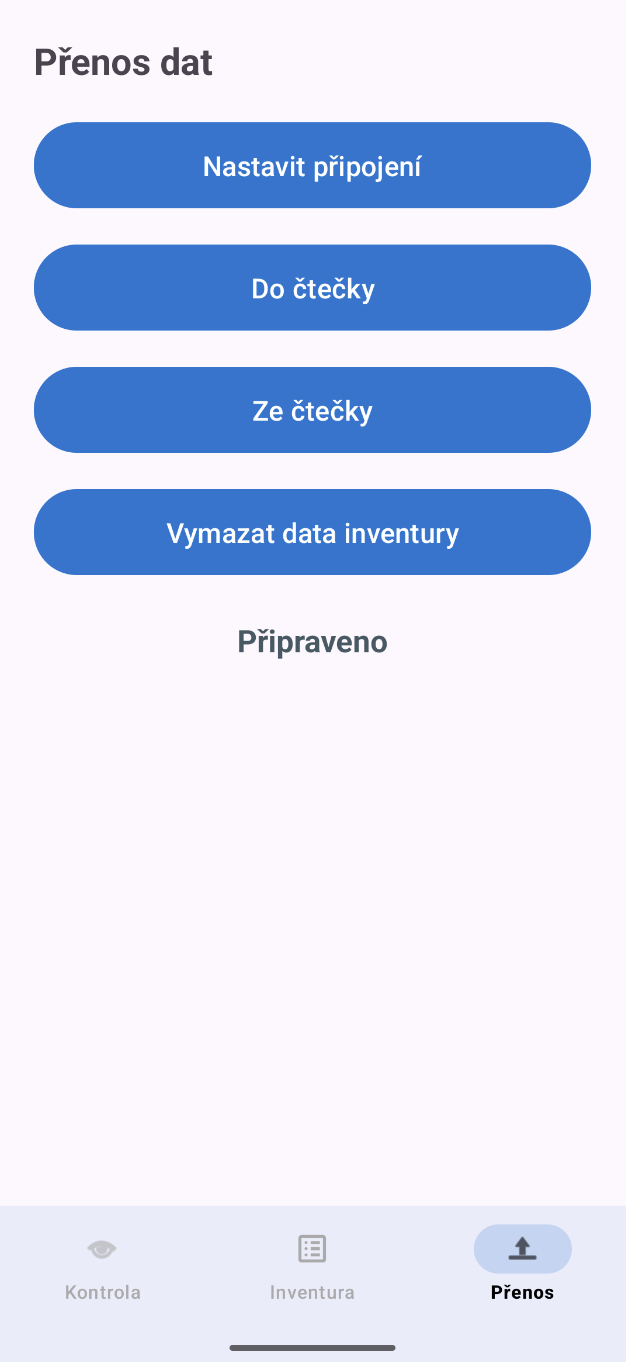
\includegraphics[width=0.35\textwidth]{images/data_transfer_page.png}
	\caption{Obrazovka přenosu dat mezi čtečkou a~serverem}
	\label{fig:data-transfer-page}
\end{figure}

\begin{figure}[H]
	\centering
	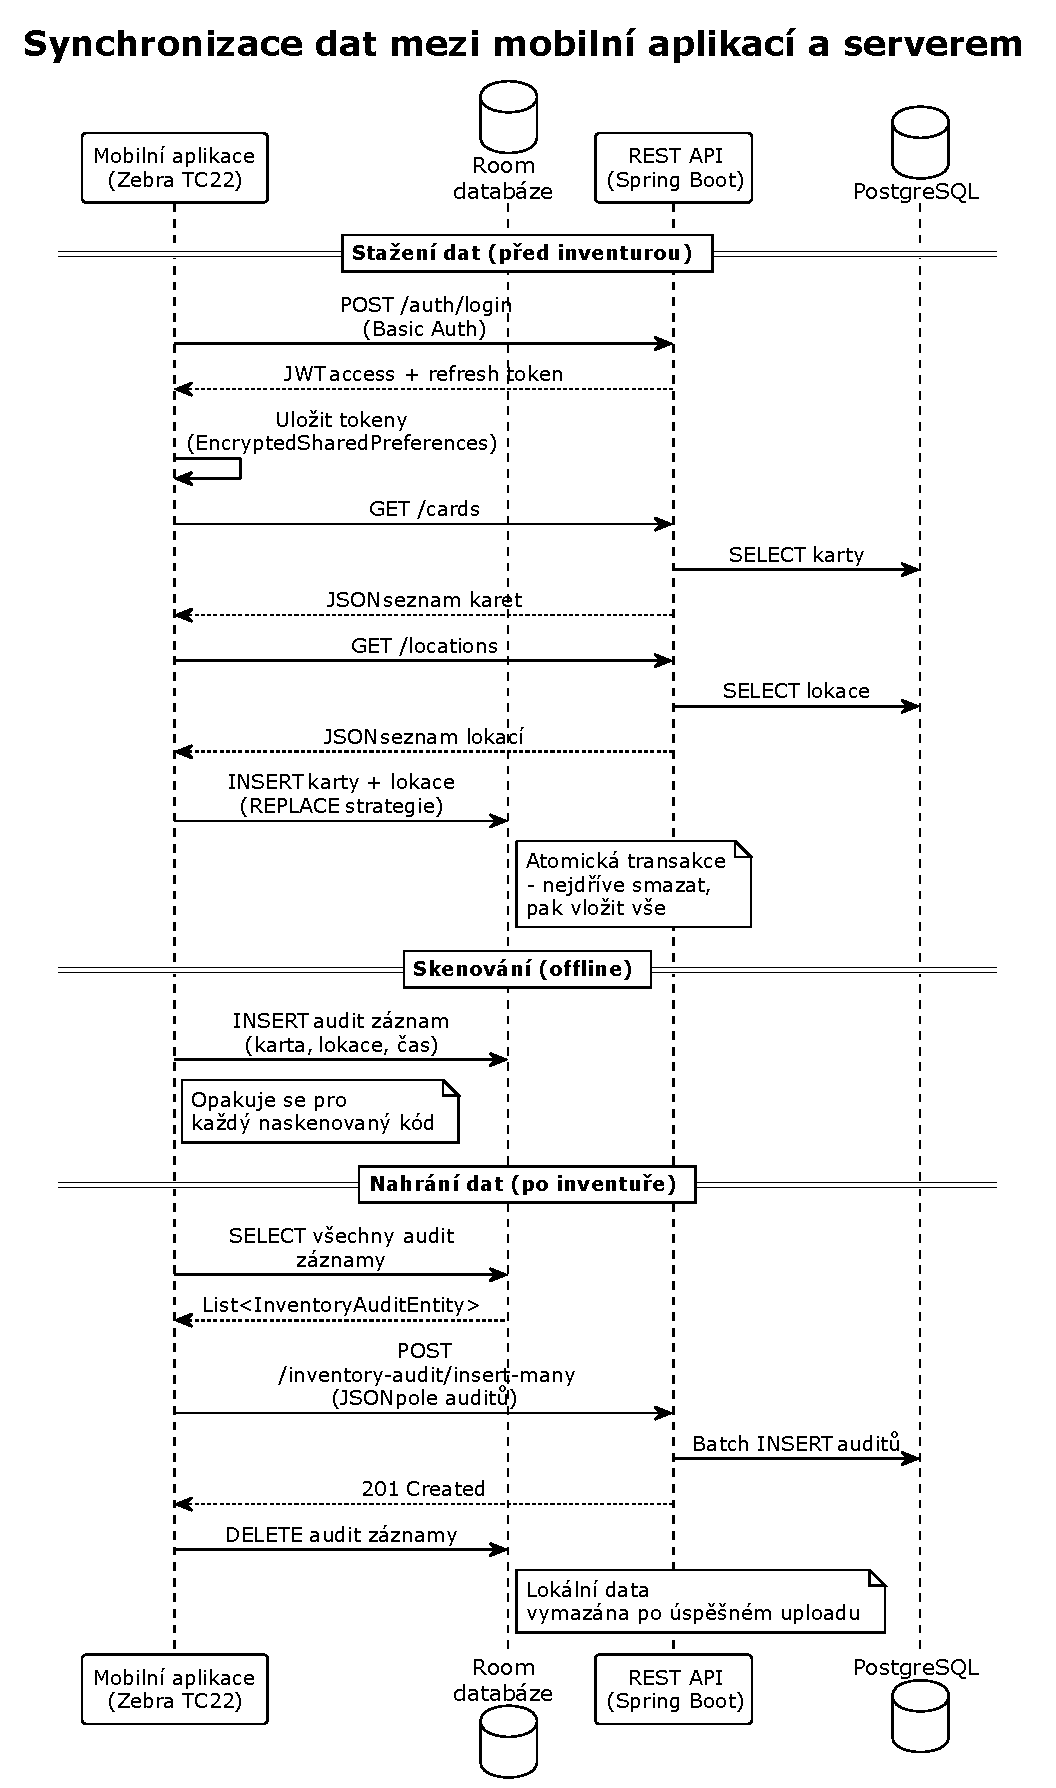
\includegraphics[width=0.85\textwidth]{images/sequence-sync.pdf}
	\caption{Sekvenční diagram -- synchronizace dat mezi mobilní aplikací a~serverem}
	\label{fig:sequence-sync}
\end{figure}

\begin{listing}[H]
\caption{Stažení dat ze serveru do lokální databáze}\label{lst:download}
\begin{minted}[fontsize=\small]{java}
public void downloadToDevice(Context ctx, Callback cb) {
  io.execute(() -> {
    try {
      String token = ensureToken(ctx);
      List<LocationEntity> locations =
          fetchLocations(ctx, token);
      List<CardEntity> cards = fetchCards(ctx, token);
      AppDatabase db = AppDatabase.getInstance(ctx);
      db.runInTransaction(() -> {
        db.cardDao().clear();
        db.locationDao().clear();
        db.locationDao().insertAll(locations);
        db.cardDao().insertAll(cards);
      });
      cb.onSuccess(cards.size());
    } catch (Exception ex) {
      cb.onError(ex.getMessage());
    }
  });
}
\end{minted}
\end{listing}

Metoda \texttt{ensureToken()} automaticky provede přihlášení prostřednictvím Basic Auth, pokud aktuální token vypršel. Stažená data jsou vložena do lokální databáze atomicky v~rámci jedné transakce -- nejprve se smažou stará data, poté se hromadně vloží nová. Stažení nových dat je zablokováno, pokud v~databázi existují neodeslaná inventurní data.

Odeslání inventury serializuje záznamy do JSON s~časovými razítky ve formátu ISO~8601 v~UTC a~odesílá je hromadným požadavkem \texttt{POST /api/inventory-audit/insert-many}.

\subsection{Bezpečnost mobilní aplikace}

Šifrování AES-256-GCM pro hodnoty a~AES-256-SIV pro klíče zajišťuje třída \texttt{EncryptedSharedPreferences}, ve~které jsou uloženy autentizační tokeny:

\begin{listing}[H]
\caption{Inicializace šifrovaného úložiště}\label{lst:tokenstorage}
\begin{minted}[fontsize=\small]{java}
private static SharedPreferences sp(Context ctx) {
  MasterKey masterKey = new MasterKey.Builder(ctx)
      .setKeyScheme(MasterKey.KeyScheme.AES256_GCM)
      .build();
  return EncryptedSharedPreferences.create(
      ctx, PREF, masterKey,
      PrefKeyEncryptionScheme.AES256_SIV,
      PrefValueEncryptionScheme.AES256_GCM);
}
\end{minted}
\end{listing}

Přihlašovací údaje uživatel zadá jednorázově v~dialogu nastavení připojení a~aplikace je uloží do stejného šifrovaného úložiště jako tokeny. Údaje tak nejsou součástí sestavené aplikace. Síťová konfigurace aplikace zakazuje nešifrovanou komunikaci (\texttt{cleartextTrafficPermitted=false}).



\chapter{Testování a~nasazení}\label{chap:testing}

\begin{chapterabstract}
	Kapitola popisuje strategii testování jednotlivých částí systému, měření pokrytí kódu, průběžnou integraci a~proces nasazení aplikace do produkčního prostředí.
\end{chapterabstract}

\section{Testování backendu}

Backend je testován na třech úrovních: unit testy izolovaných komponent, testy datové vrstvy nad in-memory databází a~integrační testy celého API. Celkem obsahuje 445 testovacích metod ve~44 testovacích třídách.

\subsection{Unit testy}

Unit testy ověřují business logiku service vrstvy a~chování kontrolerů v~izolaci. Jsou implementovány pomocí JUnit~5 a~knihovny Mockito, která umožňuje nahradit závislosti (repozitáře, mappery) simulovanými objekty (\texttt{@Mock}).

Kontrolery jsou testovány prostřednictvím \texttt{MockMvc} -- Spring testovací framework, který simuluje HTTP požadavky bez spuštění skutečného serveru. Testy ověřují správné HTTP kódy, formát odpovědí a~validaci vstupních dat. Service testy ověřují business logiku včetně chybových scénářů (neexistující entita, duplicitní identifikátor, neplatné přihlašovací údaje).

\subsection{Testy datové vrstvy}

Repozitáře a~JPA Specification jsou testovány anotací \texttt{@DataJpaTest}, která spouští pouze datovou vrstvu nad in-memory databází H2 v~PostgreSQL compatibility mode. Testy ověřují správnost dotazů odvozených z~názvů metod, explicitních \texttt{@Query} anotací a~dynamických predikátů pro filtrování karet majetku.

\subsection{Integrační testy}

Integrační testy spouštějí celou Spring Boot aplikaci (\texttt{@SpringBootTest}) včetně bezpečnostní konfigurace, serializace a~databázové vrstvy. Pokrývají kompletní API flow od autentizace přes CRUD operace až po inventurní projekci. Všechny integrační testy dědí ze~společné třídy \texttt{BaseIntegrationTest}, která zajišťuje vytvoření testovacích uživatelů a~přihlášení.

\subsection{Pokrytí kódu}

Pokrytí kódu je měřeno nástrojem JaCoCo s~následujícími minimálními prahy:

\begin{itemize}
	\item pokrytí řádků: alespoň 80\,\%,
	\item pokrytí větví: alespoň 75\,\%.
\end{itemize}

Z~měření jsou vyloučeny třídy, které neobsahují testovatelnou logiku: DTO, JPA entity, konfigurační třídy a~MapStruct mappery (generovaný kód). Konfigurace prahových hodnot je znázorněna ve~výpisu~\ref{lst:jacoco}. Při nesplnění build selže.

\begin{listing}[H]
\caption{Konfigurace JaCoCo -- minimální pokrytí kódu}\label{lst:jacoco}
\begin{minted}[fontsize=\small]{xml}
<rule>
  <element>PACKAGE</element>
  <limits>
    <limit>
      <counter>LINE</counter>
      <value>COVEREDRATIO</value>
      <minimum>0.80</minimum>
    </limit>
    <limit>
      <counter>BRANCH</counter>
      <value>COVEREDRATIO</value>
      <minimum>0.75</minimum>
    </limit>
  </limits>
</rule>
\end{minted}
\end{listing}

\section{Testování frontendu}

Frontend je testován knihovnou Vitest (7 testovacích souborů, 54 testovacích metod). Testy pokrývají kritickou business logiku -- utility funkce (formátování dat, české řazení, extrakce chybových hlášek), validační schémata a~vybrané React komponenty. Komponentové testy využívají \texttt{@testing-library/react} pro renderování a~simulaci uživatelských interakcí. Správnost UI komponent je dále zajištěna statickou typovou kontrolou TypeScriptu.

Statická typová kontrola prostřednictvím kompilátoru TypeScriptu slouží jako doplňková vrstva ověření -- při každém buildu kompilátor zkontroluje typovou konzistenci celé aplikace.

\section{Testování mobilní aplikace}

Mobilní aplikace obsahuje dva typy testů:

\begin{itemize}
	\item \textbf{Unit testy} (3 soubory) -- testují síťovou komunikaci (\texttt{ApiClient\-Test} s~knihovnou MockWebServer), synchronizační logiku (\texttt{DataSync\-Repository\-Test}) a~správu konfigurace (\texttt{BaseUrl\-Storage\-Test}). Běží na JVM bez emulátoru.
	\item \textbf{Instrumentované testy} (2 soubory) -- běží na emulátoru nebo fyzickém zařízení. Testují Room DAO operace (\texttt{DaoTest}: vkládání, dotazování, mazání, upsert) a~šifrované úložiště (\texttt{TokenStorageTest}: ukládání a~čtení tokenů, migrace z~nešifrovaného úložiště).
\end{itemize}

Uživatelské rozhraní je průběžně ověřováno manuálním testováním na cílovém zařízení Zebra TC22.

\section{Souhrn testování}

Tabulka~\ref{tab:tests} shrnuje rozsah testování všech komponent systému. U~frontendu doplňuje kompilační typová kontrola TypeScriptu dynamické testy o~statické ověření typové konzistence celé aplikace.

\begin{table}[H]\centering
\renewcommand{\arraystretch}{1.3}
\begin{tabular}{l|r|l|l}
	\textbf{Komponenta} & \textbf{Testů} & \textbf{Pokrytí kódu} & \textbf{Nástroje} \tabularnewline \hline
	Backend & 445 & $\geq$\,80\,\% ř., $\geq$\,75\,\% větví & JUnit~5, Mockito \tabularnewline
	Frontend & 54 & -- & Vitest \tabularnewline
	Mobilní apl. & 40 & -- & JUnit~5 \tabularnewline
\end{tabular}
\caption{Přehled testů jednotlivých komponent}\label{tab:tests}
\end{table}

\section{Průběžná integrace}

Projekt využívá GitHub Actions pro automatizované sestavení, testování a~statickou analýzu kódu. Workflow \texttt{sonarcloud.yml} se spouští při každém push do větve \texttt{main} a~sestává ze~čtyř kroků:

\begin{enumerate}
	\item \textbf{Backend} -- sestavení a~spuštění testů příkazem \texttt{mvn clean verify}. Výstupem jsou zkompilované třídy, výsledky testů a~JaCoCo report.
	\item \textbf{Android} -- sestavení a~spuštění unit testů. Instrumentované testy vyžadující emulátor nejsou v~CI zahrnuty a~jsou spouštěny lokálně.
	\item \textbf{Frontend} -- instalace závislostí (\texttt{npm ci}) a~spuštění testů (\texttt{npm run test}).
	\item \textbf{SonarCloud} -- po úspěšném dokončení předchozích kroků se spustí statická analýza kódu nad všemi třemi moduly. SonarCloud vyhodnocuje kvalitu kódu, bezpečnostní zranitelnosti a~duplicity.
\end{enumerate}

Zkrácená ukázka CI workflow je ve~výpisu~\ref{lst:ci}.

\begin{listing}[H]
\caption{GitHub Actions workflow pro průběžnou integraci (zkráceno)}\label{lst:ci}
\begin{minted}[fontsize=\small]{yaml}
name: SonarCloud Analysis
on:
  push:
    branches: [main]
jobs:
  backend:
    runs-on: ubuntu-latest
    steps:
      - uses: actions/checkout@v4
      - uses: actions/setup-java@v4
        with: { java-version: '21' }
      - run: mvn -B -f pom.xml clean verify
  android:
    runs-on: ubuntu-latest
    steps:
      - run: ./gradlew assembleDebug testDebugUnitTest
  frontend:
    runs-on: ubuntu-latest
    steps:
      - run: npm ci && npm run test
  sonarcloud:
    needs: [backend, android, frontend]
    steps:
      - uses: SonarSource/sonarqube-scan-action@v4
\end{minted}
\end{listing}

\section{Nasazení}

Tato sekce popisuje produkční prostředí systému: zvolenou serverovou infrastrukturu, deployment pipeline, monitoring a~způsob distribuce mobilní aplikace.

Pro provoz systému byl zvolen pronajatý VPS server s~operačním systémem Ubuntu. Oproti cloudovým platformám (AWS, Azure) toto řešení nabízí nižší provozní náklady a~plnou kontrolu nad konfigurací, což odpovídá rozsahu projektu i~technickým možnostem cílové organizace. Webová aplikace je veřejně dostupná na adrese \url{https://majetek.zs-ustavni.cz}. Architekturu nasazení znázorňuje obrázek~\ref{fig:system-architecture}.

\subsection{Serverová infrastruktura}

Serverovou infrastrukturou jsou míněny všechny komponenty běžící na VPS, které dohromady umožňují obsluhu HTTPS požadavku od uživatele -- reverse proxy, backendová aplikace, databáze a~doplňková provozní opatření (zálohy, zabezpečení vzdáleného přístupu). Architektura odpovídá běžnému třívrstvému uspořádání webové aplikace: požadavek z~prohlížeče dorazí na reverse proxy, ta obslouží statické soubory frontendu nebo přesměruje API volání na backend, který přistupuje k~datům v~databázi. Konkrétně na serveru běží tyto tři služby:

\begin{itemize}
	\item \textbf{Nginx} -- reverse proxy, která obsluhuje HTTPS požadavky. Statické soubory frontendu jsou obsluhovány přímo z~adresáře \texttt{/var/www/majetek} s~SPA fallback (\texttt{try\_files}). Požadavky na \texttt{/api/} jsou přesměrovány na backend (\texttt{proxy\_pass http://localhost:8080}). SSL certifikát je vydán autoritou Let's Encrypt s~automatickou obnovou.
	\item \textbf{Spring Boot backend} -- běží jako systemd služba na portu 8080 a~komunikuje s~databází prostřednictvím JDBC. Při výpadku ji systemd automaticky restartuje.
	\item \textbf{PostgreSQL} -- databázový server s~automatickým denním zálohováním prostřednictvím cron úlohy. Zálohy jsou uchovávány lokálně po dobu 30 dnů.
\end{itemize}

Přístup k~serveru přes SSH je zabezpečen nestandardním portem s~autentizací výhradně klíčem (heslo zakázáno). Nginx je nakonfigurován jako \uv{default server}, který pro požadavky bez očekávaného hostname (typicky při přístupu přímo přes IP adresu) vrací HTTP kód 404, čímž neúmyslně zabraňuje skenovacím botům v~indexaci aplikace.

\subsection{Monitoring a~provozní dohled}

Vzhledem k~rozsahu projektu (jedna organizace, řádově desítky uživatelských akcí denně) nebyl nasazen plnohodnotný monitorovací nástroj typu Grafana nebo Prometheus. Provozní dohled zajišťují:

\begin{itemize}
	\item \textbf{systemd journal} -- standardní výstup backendu je archivován s~rotací podle data, přístupný příkazem \texttt{journalctl}.
	\item \textbf{Nginx access a~error logy} -- ve~standardním adresáři \texttt{/var/log/nginx/} pro analýzu HTTP požadavků a~chyb.
	\item \textbf{automatický restart} -- backend se po pádu sám obnoví díky systemd nastavení.
	\item \textbf{denní zálohy databáze} -- pravidelná cron úloha vytváří dump databáze a~uchovává jej lokálně po dobu 30 dnů.
\end{itemize}

\subsection{Proces nasazení}

Backend a~frontend jsou nasazovány společně, ale odlišnými kroky -- backend je dlouhoběžný proces, který je nutné zastavit a~znovu spustit, zatímco frontend je sada statických souborů, kterou stačí synchronizovat do adresáře obsluhovaného Nginxem. Deployment workflow \texttt{deploy.yml} (spouštěný manuálně z~rozhraní GitHubu) provede následující kroky:

\begin{enumerate}
	\item Sestaví backend JAR soubor příkazem \texttt{mvn clean package}.
	\item Sestaví frontend příkazem \texttt{npm run build}.
	\item Nahraje JAR na server prostřednictvím SCP a~restartuje backendovou systemd službu.
	\item Synchronizuje frontendové soubory na server prostřednictvím rsync (přepíše obsah \texttt{/var/www/majetek}); restart Nginxu není nutný, protože soubory jsou obslouženy přímo.
\end{enumerate}

V~případě potřeby zásahu mimo workflow lze server obsloužit ručně přes SSH (např.\ pro úpravu konfigurace nebo obnovu ze~zálohy).

\subsection{Distribuce mobilní aplikace}

Mobilní aplikace je distribuována odděleně jako APK soubor, který se na cílové zařízení Zebra TC22 nahrává ručně prostřednictvím USB. Jedná se o~interní nástroj určený pro jedno konkrétní zařízení, publikace na Google Play proto není nutná.



\chapter{Závěr}\label{chap:conclusion}

Cílem práce bylo navrhnout a~implementovat kompletní systém pro správu majetku, který nahradí dosavadní excelovou evidenci v~konkrétní základní škole, umožní inventarizaci pomocí průmyslové čtečky čárových kódů a~zjednoduší tvorbu reportů pro účetnictví. Všechny stanovené cíle byly naplněny -- rešerše ukázala, že žádné z~analyzovaných řešení nepokrývá kombinaci požadavků za přijatelnou cenu, na základě konzultací s~budoucími uživateli bylo definováno 27 funkčních a~11 obecných požadavků a~vyvinutý systém je v~současné době nasazen v~produkčním prostředí.

\section*{Hlavní výsledky práce}

Systém se skládá ze~tří integrovaných komponent: serverového REST API ve Spring Bootu nad PostgreSQL, webové aplikace v~Reactu s~TypeScriptem a~nativní Android aplikace pro inventuru v~terénu. Backend je organizován jako modulární monolit s~bezpečnostním modelem založeným na JWT tokenech s~rotací refresh tokenů, frontend využívá moderní React ekosystém (TanStack Query, React Hook Form, Zod), mobilní aplikace pracuje plně offline s~lokální Room databází a~je integrována s~hardwarovou čtečkou Zebra TC22 prostřednictvím duálního zachycení vstupu.

Systém je nasazen na produkčním VPS serveru a~je veřejně dostupný na adrese \url{https://majetek.zs-ustavni.cz}; deployment pipeline je automatizována prostřednictvím GitHub Actions. Kvalita kódu je průběžně ověřována 445~backendovými testy (s~vynuceným pokrytím alespoň 80~\% řádků a~75~\% větví prostřednictvím nástroje JaCoCo), 54~frontendovými testy a~40~testy mobilní aplikace; statickou analýzu zajišťuje SonarCloud nad všemi třemi moduly.

Praktickým přínosem práce je nasazení do reálného prostředí konkrétní organizace -- škola nyní disponuje plnohodnotným systémem evidence majetku včetně tisku ZPL etiket s~Data~Matrix kódy na termotiskárně Zebra ZD621d. Systém řeší konkrétní problém, který komerční řešení buď nepokrývají vůbec (offline inventura na průmyslové čtečce), nebo pokrývají za cenu, která přesahuje možnosti rozpočtu cílové organizace.

\section*{Možnosti dalšího rozvoje}

Systém byl navržen tak, aby pokryl současné potřeby cílové organizace, a~ponechává prostor pro rozšíření v~několika směrech, které by zvýšily jeho použitelnost pro širší okruh organizací.

\paragraph{Hromadný import existujících dat.}
Migrace z~tabulkových procesorů na vyvinutý systém probíhá v~současnosti ručním zadáním každé majetkové karty. Pro organizace s~rozsáhlejší existující evidencí by bylo vhodné doplnit funkci pro hromadný import z~CSV nebo Excel souborů s~mapováním sloupců na atributy karty a~validací číselníkových hodnot. Návrhem řešení je dialog s~průvodcem -- uživatel nahraje soubor, systém detekuje sloupce, uživatel je namapuje na atributy karty a~potvrdí import; chybné řádky jsou reportovány v~přehledu před skutečným zápisem do databáze.

\paragraph{Historie změn a~auditní stopa.}
Současná evidence neuchovává historii změn jednotlivých karet -- po úpravě atributu (např.\ změně umístění) se původní hodnota přepisuje. Pro účetní účely a~kontrolní orgány by bylo přínosné zaznamenávat všechny modifikace s~časovým razítkem a~identifikací uživatele. Implementačně to lze řešit knihovnou Hibernate Envers, která automaticky verzuje JPA entity do~paralelních historizačních tabulek, případně vlastním audit listenerem psaným ad hoc nad existujícím datovým modelem.

\paragraph{Souběžná inventura více pracovníky.}
Současná architektura předpokládá jednu inventuru s~jedním zařízením -- před zahájením se data stáhnou na zařízení, po dokončení se nahrají zpět. Při větším rozsahu majetku by bylo žádoucí umožnit více pracovníkům skenovat paralelně a~výsledky průběžně synchronizovat. To vyžaduje konfliktní strategii pro situace, kdy dva pracovníci naskenují stejnou kartu (typicky last-write-wins s~časovým razítkem) a~uzamykání místností proti dvojímu zpracování.

\paragraph{Podpora RFID identifikace.}
Identifikace pomocí Data~Matrix kódů vyžaduje přímou viditelnost etikety, což u~zaplněných regálů zpomaluje skenování. RFID technologie umožňuje hromadné čtení desítek položek na vzdálenost několika metrů. Rozšíření by spočívalo v~doplnění RFID identifikátoru jako alternativy k~Data~Matrix kódu na úrovni datového modelu a~v~integraci RFID čtečky (Zebra nabízí kombinované zařízení Zebra MC3300xR) do mobilní aplikace.

\paragraph{Centralizovaná správa mobilních zařízení.}
Při nasazení na více zařízeních (např.\ pro souběžnou inventuru) se ruční instalace APK přes USB stává neudržitelnou. Řešením je nasazení Mobile Device Management platformy (např.\ Google Workspace nebo Microsoft Intune), která umožňuje vzdáleně instalovat a~aktualizovat aplikaci, vynucovat bezpečnostní politiky a~v~případě ztráty zařízení jej dálkově zablokovat.

 % include `text.tex' from `text/' subdirectory

\appendix\appendixinit % do not remove these two commands

%\chapter{Nějaká příloha}


Sem přijde to, co nepatří do hlavní části.
 % include `appendix.tex' from `text/' subdirectory

\backmatter % do not remove this command

\printbibliography[heading=bibintoc] % print out the BibLaTeX-generated bibliography list

\chapter{Obsah příloh}

	\dirtree{%
		.1 /.
		.2 README.md\DTcomment{stručný popis obsahu a~návod ke~spuštění}.
		.2 backend/\DTcomment{zdrojové kódy serverové aplikace (Spring Boot)}.
		.2 frontend/\DTcomment{zdrojové kódy webové aplikace (React)}.
		.2 android/\DTcomment{zdrojové kódy mobilní aplikace (Android)}.
		.2 thesis/\DTcomment{zdrojová forma práce ve formátu \LaTeX{}}.
	}
 % include `medium.tex' from `text/' subdirectory

\end{document}
